\documentclass[11pt,a4paper]{article}
\usepackage{fontspec}
\IfFontExistsTF{texgyrepagella-regular.otf}
 {\setmainfont{texgyrepagella}[Extension=.otf,UprightFont=*-regular,BoldFont=*-bold,
   ItalicFont=*-italic,BoldItalicFont=*-bolditalic]}
 {\IfFontExistsTF{Palatino Linotype}{\setmainfont{Palatino Linotype}}{\setmainfont{Latin Modern Roman}}}
\linespread{1.05}
\IfFileExists{spanish.ldf}
 {\usepackage[spanish,es-noshorthands,es-nodecimaldot,es-tabla]{babel}}
 {\usepackage{babel}\babelprovide[import,main,hyphenrules=nohyphenation]{spanish}\babelhyphenation[spanish]{
ab-so-lu-ta ab-so-lu-tas ab-so-lu-to ab-so-lu-tos ab-sor-be ab-sor-ben ab-sor-ber ab-sor-ber-lo
ab-sor-bien-do aba-jo abier-ta abier-to abre-via-mos ac-tual aca-ba aco-ta aco-ta-da aco-ta-das
aco-ta-do aco-ta-dos aco-ta-mos aco-ta-ron aco-tan acu-mu-la-da acu-mu-la-do ad-mi-te ad-mi-ten
ad-ver-sa-ria-les adap-ta-ti-va ade-lan-te ade-más adi-cio-na-les adi-cio-nal afec-ta afec-te
afir-ma afir-ma-ba afir-ma-cio-nes afir-ma-ción afir-ma-da ago-tan agre-gar aho-ra al-can-ce
al-can-za al-can-za-ble al-can-za-bles al-can-za-do al-can-za-dos al-gu-na al-gu-nas al-gún
al-ter-na-ti-va-men-te alea-to-rio alea-to-rios am-bas am-bos an-te-rio-res an-te-rior an-tes
an-ti-dia-go-na-les an-ti-dia-go-nal anu-la anun-cia-da aná-lo-ga aná-lo-ga-men-te apa-re-ce
apa-re-cen api-lan-do apli-ca apli-ca-ción apli-ca-do apli-ca-mos apli-can-do apli-car apli-car-las
apor-ta apor-tan apro-pia-dos apro-xi-ma apro-xi-ma-cio-nes apro-xi-ma-ción aque-lla ar-bi-tra-rio
ar-gu-men-to ar-gu-men-tos ar-ti-fi-cial aris-ta aris-tas arri-ba asi-mis-mo asig-na asig-na-cio-nes
asig-na-ción asig-na-dos asig-na-mos asig-nar asin-tó-ti-ca asin-tó-ti-cas ata-ca-das ata-ca-sen
ata-can ata-quen ata-ques au-men-ta-da au-men-ta-das au-men-tan-do au-men-tan-te au-men-tar
au-to-va-lo-res au-to-va-lor au-xi-liar aun-que aña-de aña-di-mos ba-lan-ces ban-da ban-das bas-ta
bi-yec-cio-nes bis-to-cás-ti-ca bis-to-cás-ti-co blo-que blo-ques bo-rra-das bo-rra-do bo-rrar
bor-des bre-cha ca-ben ca-jas ca-mi-no ca-nó-ni-co ca-pa-ci-dad ca-si-lla ca-si-llas ca-sos
cal-cu-la-dos cal-cu-lar cam-bia cam-bian cam-bio can-ce-la can-ce-la-cio-nes can-ce-la-ción
can-ce-lan can-di-da-ta can-di-da-tas can-di-da-to can-ti-dad car-di-nal ce-ros ce-rra-da cel-da
cen-tra-do cen-tra-dos cen-trar cen-tro cen-tros cer-ca cer-ti-fi-ca-da ci-fras ci-ta-da ci-ta-do
cier-tas cla-se cla-ses cla-ve co-cien-te co-fac-tor co-lo-ca-cio-nes co-lo-ca-ción co-lo-ca-da
co-lo-ca-das co-lo-car co-lo-res co-lum-na co-lum-nas co-me-te co-mu-nes co-mún co-ne-xo co-no-ci-da
co-pias co-ro-la-rio co-ro-nas co-rrec-ción co-rres-pon-de co-rres-pon-den co-rres-pon-dien-te
co-rres-pon-dien-tes co-tas co-te-jar coe-fi-cien-te coe-fi-cien-tes coer-ci-vi-dad coin-ci-de
coin-ci-den coin-ci-den-cias com-bi-na-cio-nes com-bi-na-to-rios com-bi-nan com-pa-ra
com-pa-ra-cio-nes com-pa-ra-ción com-pa-ra-mos com-pa-rar com-pa-ti-bi-li-dad com-pa-ti-ble
com-pa-ti-bles com-par-tan com-par-te com-par-ten com-par-ti-das com-pe-ti-dor com-pen-sa-do
com-ple-men-to com-ple-ta com-ple-ta-ble com-ple-ta-cio-nes com-ple-ta-ción com-ple-tar
com-ple-tar-la com-ple-to com-po-nen-te com-po-nen-tes com-po-si-ción con-ca-vi-dad con-cen-tra-ción
con-clu-sión con-di-cio-na con-di-cio-na-da con-di-cio-na-mien-to con-di-cio-na-mos con-di-cio-nal
con-di-cio-nal-men-te con-di-cio-ne-mos con-di-cio-nes con-di-ción con-fun-dir-la con-ge-la
con-ge-la-ción con-ge-la-da con-ge-la-das con-ge-la-mos con-ge-lar con-je-tu-ra con-je-tu-ra-da
con-jun-tas con-jun-to con-jun-tos con-se-cuen-cia con-ser-va con-ser-va-mos con-ser-van
con-si-de-ra-do con-si-de-ra-mos con-si-de-re-mos con-si-guien-te con-sis-te con-sis-ten-cia
con-ta-bi-li-za con-ta-mos con-tan-do con-tar con-tar-la con-te-ni-da con-ten-ga con-teo con-teos
con-ti-nua con-ti-nua-ción con-ti-nuas con-ti-nui-dad con-ti-nuo con-tie-ne con-tie-nen
con-tra-di-ce con-tra-dic-ción con-trac-ción con-traer con-tri-bu-cio-nes con-tri-bu-ción
con-tri-bu-ye con-tri-bu-yen con-tri-buir con-tro-la con-tro-la-do con-tro-la-mos con-tro-lar
con-trol con-ve-xa con-ve-xi-dad con-ve-xo con-ver-ge con-ver-gen-cia con-ver-sión con-vier-te
cons-ta cons-tan-tes cons-tru-yen cons-tru-yó cons-truc-ción cons-trui-do coor-de-na-da
coor-de-na-das cor-ta cor-tan cor-te cos-te cos-tes cre-cer cre-cien-tes cru-ce cru-ces cru-za-das
cru-za-dos cu-bier-tas cu-bier-to cu-bre cu-brir cu-yas cu-yos cua-dra-do cua-drá-ti-ca
cua-drá-ti-co cua-les-quie-ra cua-li-ta-ti-va cua-tro cual-quie-ra cual-quier cuan-do
cuan-ti-ta-ti-va cuar-ta cuar-to cuen-ta cuen-tan cuen-tas cuer-da cues-ta cues-tan cues-tio-nes
cum-pla cum-ple cum-plen cum-pli-ría cum-plién-do-se cuá-dru-pla cuá-dru-plas cuá-les cuán-tas
cál-cu-lo cír-cu-lo cír-cu-los da-das da-mos da-ría de-ben de-ci-mos de-cir de-cre-cien-te de-du-ce
de-du-cir-la de-fec-to de-fi-ne de-fi-nen de-fi-ni-cio-nes de-fi-ni-ción de-fi-ni-da de-fi-ni-mos
de-jan de-lan-te de-mos-tra-ción de-mos-tra-mos de-mues-tra de-mues-tran de-más de-no-mi-na-do-res
de-no-mi-na-dor de-no-ta de-no-ta-mos de-no-tan de-no-tan-do de-no-te-mos de-pen-dan de-pen-de
de-pen-den de-pen-der de-pen-dien-te de-pen-dien-tes de-re-cha de-re-cho de-ri-va de-ri-va-da
de-ri-var de-ri-vas de-sa-pa-re-ce de-sa-pa-re-cen de-sa-rro-lla-mos de-sa-rro-llo de-sa-rro-llos
de-si-gual-da-des de-si-gual-dad de-sig-na de-sig-nan de-ta-lla-mos de-te-ni-da de-te-ni-das
de-te-ni-dos de-ter-mi-na de-ter-mi-nan de-ter-mi-nan-te de-ter-mi-nar de-ter-mi-nis-ta
de-ter-mi-nis-tas de-ter-mi-nó de-tie-ne de-vol-ver den-si-dad den-tro des-car-tan-do des-con-tar
des-cri-be des-cri-bir des-cu-bier-ta des-cu-bier-tas des-cu-bier-tos des-de des-pla-za
des-pla-zar-lo des-pués des-ta-can di-bu-ja-das di-cha di-cho di-fe-ren-cia di-fe-ren-cias
di-fe-ren-tes di-fie-re di-fie-ren di-fu-sión di-rec-ción di-rec-ta di-rec-ta-men-te di-ría
di-ver-gen-cia di-vi-de di-vi-di-da di-vi-di-do di-vi-di-mos di-vi-dir di-vi-sión dia-go-na-les
dia-go-nal die-ci-séis dis-con-ti-nuas dis-cre-pan-cia dis-cre-pan-cias dis-cre-tas
dis-cre-ti-za-ción dis-cre-to dis-cre-tos dis-cu-sión dis-jun-tos dis-mi-nu-ye dis-po-ne
dis-po-ni-bi-li-da-des dis-po-ni-bi-li-dad dis-po-ni-ble dis-po-ni-bles dis-tan-cia dis-tan-cias
dis-tin-ción dis-tin-gue dis-tin-gui-da dis-tin-gui-das dis-tin-gui-mos dis-tin-ta dis-tin-tas
dis-tin-to dis-tin-tos dis-tri-bu-cio-nes dis-tri-bu-ción do-ble do-mi-na do-mi-nan do-mi-nio don-de
dé-bi-les dé-bil ecua-ción edi-to-rial efec-to ejem-plo ele-gi-da ele-gi-das ele-gi-mos ele-gir
ele-men-tos ele-va-da ele-var elec-cio-nes elec-ción eli-ge eli-gen eli-gien-do eli-mi-na
eli-mi-na-cio-nes eli-mi-na-ción eli-mi-na-da eli-mi-na-das eli-mi-nar em-pa-re-ja-da
em-pa-re-ja-das em-pa-re-ja-mien-to em-plean em-pí-ri-ca en-ci-ma en-te-ro en-te-ros en-ton-ces
en-tra-da en-tra-das en-tre en-tro-pía en-tro-pías en-tró en-tró-pi-ca enu-me-ra-ción enun-cia-do
equi-va-le equi-va-len-te-men-te erro-res es-ca-la-da es-ca-la-do es-ca-la-res es-ca-lar
es-co-ge-mos es-co-gen es-co-ger es-co-ger-se es-cri-ba-mos es-cri-be es-cri-bi-mos es-pa-cial
es-pa-cio es-pe-ra-da es-pe-ran-za es-pec-tral es-que-ma es-ta-ble-ce es-ta-cio-na-ria
es-ta-cio-na-rie-dad es-ta-cio-na-rio es-tar es-tas es-ti-ma es-ti-ma-cio-nes es-ti-ma-ción
es-ti-mar es-tos es-tric-ta es-tric-ta-men-te es-tu-dian es-tán es-tén eti-que-ta eti-que-tas
eu-clí-dea eva-lua-ción eva-lua-da eva-lua-dos eva-lúa eva-lúan ex-cep-cio-na-les ex-cep-cio-nal
ex-cep-cio-nes ex-cep-ción ex-clu-sión ex-clu-ye-ron ex-cluir ex-hi-bi-dos ex-pan-sión ex-pli-ca
ex-plí-ci-to ex-po-nen-cial ex-po-nen-ciar ex-po-nen-te ex-pre-sa ex-te-rio-res ex-te-rior
ex-ten-de-mos ex-ten-di-da ex-ten-di-do ex-ten-di-dos ex-ten-sión ex-trac-tos ex-trae ex-trae-mos
ex-traer ex-tre-mo ex-tre-mos exac-ta exac-ta-men-te exac-to exac-tos exi-ge exi-gir exi-to-sa
exi-to-sas exis-te exis-ten fa-lla-ría fa-lla-se fa-lle fa-llo fa-mi-lia fa-mi-lias fac-ti-ble
fac-ti-bles fac-to-res fac-to-ri-za-ción fac-to-ria-les fac-tor fal-ta fe-nó-me-no fi-bra fi-bras
fi-gu-ra fi-gu-ran fi-ja-da fi-ja-das fi-ja-do fi-ja-dos fi-ja-mos fi-jan fi-jar fi-jas fi-je-mos
fi-jos fi-las fi-nal fi-nal-men-te fi-nas fi-ni-ta fi-ni-to fic-ti-cias fic-ti-cio fic-ti-cios
for-ma for-ma-do for-man for-mar for-mas frac-ción fue-ra fuen-tes fuer-za fun-cio-na-les
fun-cio-nes fun-ción fí-si-ca fí-si-cas fí-si-co fí-si-cos fór-mu-la fór-mu-las ga-ran-ti-zar gau-ge
ge-ne-ra-das ge-ne-ral ge-ne-ran geo-me-tría geo-mé-tri-ca geo-mé-tri-cas geo-mé-tri-co glo-bal
gra-dien-te gra-do gra-dos gra-fo gran-de gran-des grue-sa ha-bría ha-ce-mos ha-cer-la ha-ría ha-yan
has-ta he-chos he-re-da he-re-dan he-ren-cia he-rra-mien-tas hes-sia-na hi-jos hi-per-pla-nos
hi-pó-te-sis his-to-ria his-to-rias ho-ri-zon-ta-les hu-bie-se iden-ti-da-des iden-ti-dad
iden-ti-fi-ca iden-ti-fi-ca-ción iden-ti-fi-can idén-ti-ca igua-les igual-da-des igual-dad
}

\babelhyphenation[spanish]{
iden-ti-fi-can idén-ti-ca igua-les igual-da-des igual-dad igual-men-te ilus-tra im-pli-ca im-po-ne
im-po-nen im-po-ner im-po-si-ble ima-gen in-ci-de in-ci-den-cia in-ci-den-te in-ci-den-tes
in-clu-si-ve in-clu-sión in-clu-so in-clu-ye in-clu-yen-do in-clui-da in-clui-do in-clui-mos
in-cor-po-rar-se in-cre-men-to in-cre-men-tos in-cum-plir in-de-pen-den-cia in-de-pen-dien-te
in-de-pen-dien-te-men-te in-de-pen-dien-tes in-de-xa-mos in-di-ca in-di-ca-do-res in-di-ca-dor
in-di-can in-di-vi-dua-les in-di-vi-dual in-du-ce in-fe-rior in-fe-rior-men-te in-fi-ni-to
in-for-ma-ción in-me-dia-ta-men-te in-me-dia-to in-ser-cio-nes in-ser-ción in-ser-ta in-ser-tan
in-ser-tar in-te-gra in-te-gra-ción in-te-gra-do in-te-gra-dos in-te-gra-mos in-te-gral
in-te-gran-do in-te-grar in-te-li-gen-cia in-te-rior in-ter-cam-bian in-ter-cam-biar
in-ter-sec-cio-nes in-ter-sec-ción in-ter-va-lo in-ter-va-los in-ter-vie-ne in-ter-vie-nen
in-tro-duc-ción in-ver-sa in-ver-sas in-ver-sión in-yec-ti-va in-yec-ti-vas inal-te-ra-das
ini-cia-da ini-cial ini-cio ins-tan-te ite-ra-mos iz-quier-da iz-quier-do jun-to jus-ti-fi-ca
la-pla-cia-no lar-go le-ga-les le-ga-li-dad le-gal le-tra le-tras le-yes li-bre li-bres li-mi-ta-do
li-nea-les li-neal lla-ma-mos lle-ga lle-ga-da lle-gar lle-gue lle-no lo-ca-les lo-cal lo-ga-rit-mo
lo-ga-rit-mos lon-gi-tu-des lon-gi-tud lu-gar lue-go lí-mi-te lí-mi-tes lí-nea lí-neas
ma-cros-có-pi-ca ma-cros-có-pi-cas ma-cros-có-pi-co ma-cros-có-pi-cos ma-ne-ra ma-ne-ras ma-sas
ma-tri-ces ma-tri-cial ma-triz ma-xi-mal ma-xi-mi-za-dor ma-yo-res ma-yor man-tie-nen mar-ca
mar-gi-na-les mar-tin-ga-la mar-tin-ga-las me-di-da me-di-mos me-dia me-dian-te me-dias me-nor
me-nos me-sos-có-pi-co mi-ni-mi-za-dor miem-bro mien-tras mis-ma mis-mas mis-mo mis-mos mix-ta
mo-de-lo mo-di-fi-ca mo-no-to-nía mo-ti-va mue-ve mues-tra mues-tran mul-ti-pli-ca mul-ti-pli-ca-da
mul-ti-pli-ca-do mul-ti-pli-ca-do-res mul-ti-pli-ca-dor mul-ti-pli-ca-mos mul-ti-pli-ca-ti-va
mul-ti-pli-ca-ti-vo mul-ti-pli-can-do mul-ti-pli-car mul-ti-pli-car-lo má-xi-mo má-xi-mos más-ca-ra
mé-to-dos mí-ni-ma mí-ni-mo mó-du-lo mó-du-los ne-ce-sa-rio ne-ce-si-ta ne-ce-si-ta-mos ne-ga-ti-va
ne-ga-ti-vas ne-ga-ti-vo nin-gu-na nin-gu-no nin-gún no-ta-cio-nes no-ta-ción nor-ma
nor-ma-li-za-cio-nes nor-ma-li-za-ción nor-ma-li-za-da nor-ma-li-za-do nor-ma-li-za-do-res
nor-ma-li-za-dor nor-ma-li-zar nor-mas nu-las nu-los nu-me-ra-dor nu-me-ra-mos nu-me-ran
nu-mé-ri-ca-men-te nue-vo nú-cleo nú-me-ro nú-me-ros ob-je-ti-vo ob-je-ti-vos ob-je-tos ob-ser-va
ob-ser-va-ble ob-ser-va-bles ob-ser-va-cio-nes ob-ser-va-ción ob-ser-ve-mos ob-te-ne-mos ob-te-ner
ob-ten-dría ob-tie-ne ob-tie-nen ob-tu-vo obli-cuas ocu-pa ocu-pa-ción ocu-pa-da ocu-pa-das ocu-par
ocu-rre op-cio-nes op-ti-mi-zar ope-ra-ción ope-ra-dor opues-tos or-de-na-das or-de-na-dos
or-de-na-mos or-den or-di-na-ria or-di-na-rias or-di-na-rio or-ga-ni-zar or-to-go-na-les
or-to-go-na-li-dad or-to-go-nal or-to-nor-ma-les or-to-nor-mal ori-gen ori-gi-na-les ori-gi-nal
os-ci-la-ción pa-dre pa-dres pa-la-bra pa-la-bras pa-ra-da pa-ra-das pa-ra-mos pa-rar pa-rar-la
pa-re-mos pa-res pa-rá-me-tro pa-rá-me-tros pa-san pa-san-do pa-sar pa-sos pa-tro-nes pa-trón
par-cial par-te par-ti-ción par-ti-cu-lar par-ti-mos par-tir pe-que-ña pe-que-ñas pe-que-ño
pe-que-ños pe-sos per-der per-der-la per-ma-nen-cia per-ma-nen-te per-ma-nen-tes per-mi-te
per-mu-ta-cio-nes per-mu-ta-ción per-te-ne-ce per-te-ne-cen per-te-nez-can per-tur-ba-cio-nes
per-tur-ba-ción pi-den pi-vo-te pi-vo-tes pie-za pie-zas pier-den plan-tea pma-trix po-cas po-de-mos
po-li-nó-mi-co po-ne-mos po-si-bi-li-da-des po-si-bles po-si-cio-nes po-si-ción po-si-ti-va
po-si-ti-vas po-si-ti-vi-dad po-si-ti-vo po-si-ti-vos po-ten-cia pon-de-ra-da pon-de-ra-das
pon-de-ra-do pon-de-rar pon-ga-mos por-que pre-ci-sa pre-ci-sa-men-te pre-ci-sar pre-ci-sión
pre-de-ci-ble pre-dic-ción pre-dic-to-res pre-fi-jo pre-fi-jos pre-gun-ta pre-pa-rar pre-ser-va
pre-ser-ve pre-su-pues-to pre-via pres-cri-be pres-cri-ta pres-cri-tas pres-cri-to pres-cri-tos
pres-crip-cio-nes pri-me-ra pri-me-ras pri-me-ro pri-me-ros pri-mer prin-ci-pal pro-ba-bi-li-da-des
pro-ba-bi-li-dad pro-ba-da pro-ba-mos pro-bar pro-ble-ma pro-bó pro-ce-so pro-du-ce pro-du-cen
pro-du-je-ra pro-duc-to pro-duc-to-ria pro-duc-tos pro-gre-sio-nes pro-hi-bi-da pro-lon-ga
pro-lon-ga-da pro-lon-gan pro-me-diar pro-pia pro-pie-dad pro-pio pro-po-si-ción pro-por-cio-na
pro-por-cio-nal pro-por-cio-nan pro-por-cio-nes pro-vie-ne pro-yec-cio-nes pro-yec-ción
pro-yec-to-res prue-ba prue-ban prue-bas pró-xi-ma pseu-do-de-ter-mi-nan-te pue-da pue-de pue-den
pues-to pun-to pun-tos pér-di-da que-da que-dan que-dar que-pa que-pan ra-dio ra-zo-nes ran-go
re-ci-be re-cién re-co-rre re-co-rren re-cons-truc-ción re-cor-da-mos re-cu-pe-ra re-cu-pe-rar
re-cur-sión re-cí-pro-ca-men-te re-don-da re-don-deo re-du-ce re-du-cen re-du-cien-do re-du-cir
re-duc-ción re-fe-ren-cia re-fi-na-mien-to re-fi-nar re-gio-nes re-gis-tra-mos re-gión re-gla
re-gu-la-res re-gu-la-ri-dad re-gu-la-ri-za-do re-gu-lar re-la-cio-na-das re-la-ción re-la-ti-va
re-la-ti-va-men-te re-la-ti-vas re-la-ti-vo re-pe-ti-das re-pi-te re-pi-ten re-pre-sen-ta-ción
re-pre-sen-tan re-pre-sen-tan-te re-que-ri-da re-que-rir re-quie-re re-ser-va-mos re-si-dua-les
re-si-dual re-sol-ve-mos re-sol-ven-tes re-suel-ve re-sul-ta re-sul-ta-do re-sul-ta-dos
re-sul-tan-te re-ti-rar re-tí-cu-la re-ve-la re-ve-la-da re-ve-la-das re-ve-la-do re-ve-la-mos
re-ve-lar re-ver-si-ble re-vi-sio-nes rea-les rea-li-zar rec-tan-gu-lar rec-tas rec-tán-gu-lo
rec-tán-gu-los ree-qui-li-bra-do rees-truc-tu-ra-ción rei-na rei-nas res-pe-ta res-pec-ti-va-men-te
res-pec-ti-vas res-pec-to res-ta res-ta-mos res-tan res-tan-te res-tan-tes res-tar res-to res-tos
res-tric-cio-nes res-tric-ción res-trin-gi-do res-trin-gi-mos res-trin-gien-do reu-nien-do reu-nir
reú-ne ro-dea-dos sa-li-da sa-tis-fa-ce sa-tis-fa-cen sa-tis-fa-cer-las sal-to sal-vo se-gun-da
se-gun-do se-guía se-gún se-lec-cio-na-da se-lec-cio-nar se-mi-de-fi-ni-da se-mi-de-fi-ni-das
se-mi-de-fi-ni-do se-pa-ra-da se-pa-ra-do se-pa-ra-dos se-pa-ran-do se-rie se-ría se-ña-la
se-ña-la-do se-ña-lan sec-cio-nes sec-ción seg-men-to si-gue si-guen si-guien-te si-me-tría
si-mul-tá-nea si-mul-tá-nea-men-te si-mé-tri-ca si-tua-ría si-túa si-túan sie-te siem-pre sien-do
sig-no sig-nos sin-gu-la-res sin-gu-lar sir-ven sis-te-ma small-ma-trix so-bre so-bre-vi-va
so-bre-vi-van so-bre-vi-ven so-bre-vi-vir so-breen-tien-de so-la-men-te so-lu-cio-nes so-lu-ción
so-por-te sor-tea-mos su-bes-pa-cio su-bín-di-ce su-bín-di-ces su-ce-si-vas su-ce-sio-nes su-ce-sión
su-ce-so su-ce-sos su-fi-cien-te-men-te su-ma-do su-ma-mos su-man su-man-do su-man-dos su-mar su-mas
su-mán-do-las su-pe-ran su-pe-rio-res su-pe-rior su-pe-rín-di-ce su-per-mar-tin-ga-la
su-per-vi-ven-cia su-pon-ga-mos su-pre-ma su-pri-mien-do su-pri-mir sub-con-jun-to sub-con-jun-tos
sub-fi-bras sub-sec-ción sue-lo sus-ti-tu-ción sus-ti-tu-ye sus-ti-tu-yen-do sus-ti-tui-mos
sus-ti-tuir sus-ti-tuir-lo sus-tra-yen-do ta-bla ta-ble-ro ta-ble-ros ta-les ta-ma-ño ta-ma-ños
ta-sas tam-bién tan-gen-te tan-to te-les-có-pi-ca-men-te te-ne-mos te-ner te-nían tem-po-ra-les
tem-po-ral ten-der ten-dría ten-ga ten-gan teo-re-ma teo-re-mas ter-ce-ra ter-mi-na ter-mi-nal
tes-ti-go tes-ti-gos tex-to tex-tua-les ti-pos tie-ne tie-nen tiem-po tiem-pos tien-de to-da-vía
to-das to-dos to-le-ran-cia to-le-ran-cias to-ma-do to-ma-mos to-man to-man-do to-mar to-mar-se
to-me-mos to-rres to-tal tra-ba-jo tra-mo tra-ta-do tra-yec-to-ria tra-yec-to-rias tra-za tra-zan
tran-si-ción trans-fe-rir trans-fie-re trans-ver-sal tras-pues-ta trian-gu-lar trun-ca-da tér-mi-no
tér-mi-nos tó-me-se ul-ti-mas um-bra-les um-bral uni-da-des uni-dad uni-dos uni-for-me
uni-for-me-men-te uni-for-mes uni-for-mi-dad uni-ta-rio usa-dos usa-mos usa-ron usan-do use-mos
uti-li-za uti-li-za-ron uti-li-zan uti-li-zar va-can-cia va-can-cias va-cía va-cías va-cío va-cíos
va-len va-lien-do va-lo-res va-lor va-ria-ble va-ria-bles va-ria-cio-nal va-ria-ción va-rias val-gan
ve-ces ve-ci-nas ve-ci-nos ve-lo-ci-dad ve-ri-fi-ca-mos ve-ri-fi-can ve-ri-fi-car vec-to-res vec-tor
ver-sio-nes ver-ti-ca-les vie-ne vio-le vir-tua-les vir-tual vo-lú-me-nes vol-ver vér-ti-ce
vér-ti-ces áto-mo és-tas ín-di-ce ín-di-ces óp-ti-mo ór-de-nes úl-ti-ma úl-ti-mas úl-ti-mo úni-ca
úni-ca-men-te úni-co
}

}
\usepackage{amsmath,amssymb,amsthm,mathtools}
\usepackage{unicode-math}
\IfFontExistsTF{texgyrepagella-math.otf}%
{\setmathfont{texgyrepagella-math.otf}}{\setmathfont{Latin Modern Math}}
\usepackage[margin=26mm]{geometry}
\IfFileExists{microtype.sty}{\usepackage{microtype}}{}
\IfFileExists{titlesec.sty}{\usepackage[nobottomtitles*]{titlesec}
  \renewcommand{\bottomtitlespace}{.12\textheight}}{}
\usepackage{booktabs,array}
\usepackage[shortlabels]{enumitem}
\usepackage{tikz}
\usetikzlibrary{arrows.meta,positioning}
\usepackage{xcolor}
\usepackage[colorlinks=true,linkcolor={blue!45!black},citecolor={green!35!black},%
urlcolor={blue!55!black}]{hyperref}

\AtBeginDocument{\renewcommand{\tablename}{Tabla}}
\setlength{\parindent}{1.15em}
\setlength{\parskip}{0pt plus .35pt}
\setlength{\textfloatsep}{14pt plus 3pt minus 3pt}
\setlength{\intextsep}{12pt plus 3pt minus 3pt}
\setlength{\abovecaptionskip}{6pt}
\setlength{\belowcaptionskip}{2pt}
\makeatletter % barrera de flotantes, como \FloatBarrier de placeins
\providecommand\FloatBarrier{\par\begingroup\let\@elt\relax
  \edef\@tempa{\@botlist\@deferlist\@dbldeferlist}%
  \ifx\@tempa\@empty\endgroup\else\endgroup\newpage\fi\suppressfloats[t]}
\makeatother
\AtBeginDocument{\setlength{\abovedisplayskip}{9pt plus 2pt minus 3pt}%
  \setlength{\belowdisplayskip}{9pt plus 2pt minus 3pt}}
\clubpenalty=7000
\widowpenalty=7000
\displaywidowpenalty=3000
\definecolor{btinta}{HTML}{223B49}
\definecolor{bgris}{HTML}{DDE6E7}
\definecolor{bpapel}{HTML}{FFFFFF}
\newcommand{\bcuadricula}[1]{%
  \fill[bpapel] (0,0) rectangle (#1,#1);
  \foreach \r in {1,...,#1}{%
    \foreach \c in {1,...,#1}{%
      \ifodd\numexpr\r+\c\relax
        \fill[bgris] (\c-1,#1-\r) rectangle (\c,#1-\r+1);
      \fi
    }
    \node[font=\scriptsize,anchor=east] at (-.10,#1-\r+.5) {\r};
    \node[font=\scriptsize,anchor=south] at (\r-.5,#1+.06) {\r};
  }
  \foreach \t in {0,...,#1}{\draw[black!45,line width=.3pt] (\t,0)--(\t,#1) (0,\t)--(#1,\t);}
  \draw[btinta,line width=.6pt] (0,0) rectangle (#1,#1);
}
\newcommand{\breina}[3]{%
  \begin{scope}[shift={(#3-.5,#1-#2+.50)}]
    \fill[bpapel] (0,0) circle[radius=.36];
    \fill[btinta] (-.29,.15)--(-.13,.04)--(0,.30)--(.13,.04)--(.29,.15)--(.18,-.15)--(-.18,-.15)--cycle;
    \fill[btinta] (-.21,-.22) rectangle (.21,-.18);
  \end{scope}
}
\newcommand{\bmarca}[3]{\fill[btinta!62] (#3-.5,#1-#2+.50) circle[radius=.055];}

\setlength{\emergencystretch}{2em}
\allowdisplaybreaks[2]
\numberwithin{equation}{section}

\theoremstyle{plain}
\newtheorem{teorema}{Teorema}[section]
\newtheorem{proposicion}[teorema]{Proposición}
\newtheorem{lema}[teorema]{Lema}
\newtheorem{corolario}[teorema]{Corolario}
\theoremstyle{definition}
\newtheorem{definicion}[teorema]{Definición}
\newtheorem{conjetura}[teorema]{Conjetura}
\theoremstyle{remark}
\newtheorem{observacion}[teorema]{Observación}

\newcommand{\eps}{\varepsilon}
\newcommand{\ind}{\mathbf{1}}
\DeclareMathOperator{\pdet}{pdet}
\DeclareMathOperator{\diag}{diag}
\DeclareMathOperator{\tr}{tr}
\newcommand{\Cpred}{C_{\rm pred}}
\newcommand{\Qpred}{Q_{\rm pred}}

\newcommand{\E}{\mathbb{E}}
\newcommand{\Prob}{\mathbb{P}}
\DeclareMathOperator{\per}{per}

\title{El término constante del problema de las $n$ reinas}
\author{Dilan Steven Mejia\thanks{\href{mailto:mejiadilan@hotmail.com}{\nolinkurl{mejiadilan@hotmail.com}}}}
\date{}
\hypersetup{pdftitle={El término constante del problema de las n reinas},
 pdfauthor={Dilan Steven Mejia}, pdflang={es},
 pdfsubject={Problema de las n reinas. MSC 2020: 05A16, 05A05, 60C05, 94A17, 15A15},
 pdfkeywords={problema de las n reinas, enumeración asintótica, término constante, entropía relativa,
 permanente}}
\begin{document}
\maketitle
\begin{abstract}
\noindent Sea $Q(n)$ el número de colocaciones de $n$ reinas sin ataques en un tablero de
$n\times n$. Simkin determinó $\log Q(n)$ salvo un error $o(n)$ mediante un problema variacional. Un
trabajo anterior construyó, a partir de una entropía de Bethe, el predictor canónico
$Q_{\rm pred}(n)$ y obtuvo su término constante $C_{\rm pred}$, pero dejó abierto si éste es también
el término constante del conteo exacto. Probamos que lo es:
\[
\begin{aligned}
 \log Q(n)-\log n!-n\Phi &\longrightarrow C_{\rm pred},\\
 C_{\rm pred} &=\tfrac12\log2-\tfrac12-\tfrac32I_2-\tfrac12\log{\det}_2(I+J).
\end{aligned}
\]
Aquí $\Phi=s_1+1$, donde $s_1$ es el valor óptimo en masa uno, que alcanza el perfil de masa uno;
$I_2$ es la integral del cuadrado de ese perfil y $J$ es el operador de Hilbert--Schmidt construido
a partir de él. Equivalentemente, $Q(n)\sim e^{C_{\rm pred}}\,n!\,e^{n\Phi}$ y
$\log Q(n)-\log Q_{\rm pred}(n)\to0$; la cota $O(1/n)$ para esta diferencia, conjeturada en ese
trabajo, sigue abierta.

\smallskip\noindent La prueba compara dos leyes para el proceso que inserta una reina por fila, en
un orden uniforme de las filas: la ley uniforme, que revela una solución uniforme, y la ley
adaptativa, que elige cada casilla según el predictor del tablero resultante. Ese trabajo probó que
el predictor satisface la recursión del conteo salvo un factor $e^{O(k^{-2})}$ en dos clases de
tableros con $k$ filas vacías. Con esa consistencia, una identidad entrópica reduce la comparación
de los conteos al tablero en que se detiene el proceso. Bajo la ley adaptativa, los tableros
satisfacen hasta que quedan $K$ filas vacías unas condiciones que los mantienen en esas clases,
salvo probabilidad $O(e^{-cK})+o(1)$, y acotamos el coste en el primer tablero que deja de
satisfacerlas. Bajo la ley adaptativa, la probabilidad de llegar a $K$ filas vacías sin una salida
y de que dos cruces vacíos compartan diagonal es $O(K^4/n)$. Un cruce vacío es la intersección de
una fila vacía y una columna vacía. Cuando el proceso llega a $K$ sin una salida y ningún par de
cruces vacíos comparte diagonal, el conteo es un permanente, al que aplicamos la estimación de
McCullagh en la forma uniforme probada por Divoux y Wang.

\smallskip\noindent Numéricamente, $C_{\rm pred}\approx0{,}9401$, sin cota de error certificada; los
conteos exactos para ${16\le n\le27}$ son compatibles con el teorema, que no da velocidad de
convergencia.

\medskip\noindent
\textbf{Palabras clave:} problema de las $n$ reinas; enumeración asintótica; término constante;
entropía relativa; permanente.

\noindent
\textbf{MSC 2020:} 05A16; 05A05; 60C05; 94A17; 15A15.
\end{abstract}

\section{Introducción}
El problema de las $n$ reinas pregunta cuántas maneras hay de colocar $n$ reinas en un
tablero de $n\times n$ sin que dos se ataquen. Denotamos ese número por $Q(n)$ y contamos
por separado las soluciones relacionadas por una simetría. Leer las columnas de sus reinas
por orden de filas identifica cada solución con una permutación. Las restricciones diagonales
determinan cuáles de las $n!$ permutaciones sirven.

Simkin~\cite[Teorema~1.1]{simkin} obtuvo el orden principal de $\log Q(n)$ mediante
un problema variacional. Los resultados de Luria y Simkin~\cite{ls} y de Bowtell y
Keevash~\cite{bk} estudian el conteo por métodos combinatorios. Nobel, Agrawal y Boyd~\cite{nab}
acotaron la constante de primer orden. Para determinar el factor multiplicativo que queda en
el conteo después de extraer el término principal hace falta una estimación más precisa.

Sea $Q_{\rm pred}(n)$ el predictor canónico de~\cite{pred} y pongamos
$R_Q(n)=\log Q(n)-\log Q_{\rm pred}(n)$. El siguiente resultado establece que
$R_Q(n)\to0$, la forma cualitativa de la Conjetura~10.1 de~\cite{pred}.
\begin{teorema}[Término constante del conteo]\label{princ}
En el tablero ordinario, cuando $n\to\infty$,
\[
 \log Q(n)-\log n!-n\Phi\longrightarrow
 \tfrac12\log2-\tfrac12-\tfrac32 I_2-\tfrac12\log{\det}_2(I+J)=C_{\rm pred}.
\]
\end{teorema}
Aquí $\nu_1$ es el perfil óptimo de masa uno de~\cite{perfil}, $\Phi=s_1+1$ con $s_1$ su entropía, e
$I_2=\int_{[0,1]^2}\nu_1^2$. El operador $J$ es el de (D3.6) de~\cite{pred}, y su determinante
regularizado se describe en (D4.1) de ese trabajo. Un error que tiende a cero en el logaritmo
equivale a un cociente de conteos que tiende
a uno. La estimación cuantitativa $|R_Q(n)|\le C/n$ de la misma conjetura sigue abierta.

En la Sección~9 de~\cite{pred} se estima $C_{\rm pred}\approx0{,}9401$, y la evaluación directa de
la fórmula da $0{,}940144$; ninguna de las dos cifras tiene cota de error certificada. Con la
referencia $\Phi_0=1-1{,}944001$ de esa sección, los conteos exactos para $16\le n\le27$ dan
$\log Q(n)-\log n!-n\Phi_0$ entre $0{,}913$ y $0{,}941$ \cite[Tabla~2]{pred}, y $R_Q(n)$ vale
$0{,}0208$ en $n=20$ y $0{,}0119$ en $n=27$. Estos valores son compatibles con el
Teorema~\ref{princ}, pero ningún cálculo en valores finitos de $n$ lo comprueba, porque el
teorema afirma un límite sin velocidad de convergencia.

La Sección~10 de~\cite{pred} identifica tres cuestiones. La primera es la regularidad de
los tableros residuales a lo largo del proceso aleatorio. La segunda es el efecto de las
últimas filas, donde quedan pocas opciones de inserción. La tercera es cómo reunir los errores
de las sucesivas inserciones al comparar ambos conteos.

\paragraph{Esquema de la demostración.}
Escribimos $g(B)=\log Q(B)-L(B)$, donde $L(B)$ es el predictor de un tablero residual $B$
(Sección~\ref{leyes}). Hay que probar que $g(B_0)\to0$ en el tablero inicial $B_0$. Comparamos dos
leyes sobre las historias que insertan una reina por fila, en un orden uniforme de las filas. La ley
uniforme $\mu$ revela una solución uniforme. La ley adaptativa $\nu$ elige cada casilla $e$ con
probabilidad proporcional a $\exp L(B+e)$, la predicción del tablero que resulta. La
Sección~\ref{historias} expresa $g(B_0)$ con ambas leyes en una historia detenida: una identidad con
la entropía relativa de $\mu$ respecto de $\nu$ y una cota inferior bajo $\nu$. El término acumulado
de esas fórmulas es pequeño por la consistencia de~\cite{pred}.

Fijamos $\delta>0$ pequeño y un entero $K$ grande, y ponemos $M=\lceil\delta n\rceil$. El orden en
que se eligen las constantes está en la Sección~\ref{meso:constantes}. Las Secciones~\ref{macro}
y~\ref{meso} prueban que, bajo $\nu$, los tableros de la historia son regulares
(Definición~\ref{def:regular}) hasta que quedan $K$ filas vacías, salvo probabilidad
$O(e^{-cK})+o(1)$: primero mientras quedan al menos $M$ filas y después entre $M$ y $K$. La
Sección~\ref{costes} acota por arriba $g$ en el primer tablero que deja de ser regular. La
Sección~\ref{terminal} prueba que, en el tablero de $K$ filas, el conteo es un permanente fuera de
un suceso de probabilidad $O(K^4/n)$, y que allí $g$ tiende a cero al crecer $K$. En la
Sección~\ref{balance} se hace primero $n\to\infty$ con $\delta$ y $K$ fijos y después $K\to\infty$.

Los Teoremas~1.1--1.3, la Proposición~5.2 y el Teorema~7.7 de~\cite{perfil} proporcionan el
perfil continuo y sus cotas. La comparación entrópica del Teorema~3.6 de~\cite{ultimas}
motiva el argumento de la Sección~\ref{costes}, donde verificamos las estimaciones sobre el
soporte de cada residual. Usamos los Teoremas~7.1 y~8.1 y el Corolario~7.2 de~\cite{pred}
para las inserciones, y sus Teoremas~1.1 y~5.7 para la constante. La única estimación
asintótica de permanentes que usamos es la de McCullagh~\cite{mccullagh}, en la forma uniforme
probada por Divoux y Wang~\cite[Proposición~3.1 y Observación~2.1]{dw}. En la
Sección~\ref{permanente} verificamos sus hipótesis tras escalar la matriz del residual.

\section{El tablero y las leyes sobre historias}\label{leyes}
\begin{definicion}[Tablero residual]
Numeramos filas y columnas desde uno, con filas de arriba abajo y columnas de izquierda a
derecha. La casilla $(i,j)$ pertenece a $R_i,C_j,D_{i-j},A_{i+j-1}$. En las coordenadas
de~\cite{perfil,ultimas}, esta casilla es $(i-1,j-1)$, con la misma diferencia y con suma
$i+j-2$. Una diagonal, de cualquiera de las dos familias, está \emph{libre} cuando no contiene una
reina. Una línea está \emph{disponible} si es una fila o una columna vacía o una diagonal libre. El
tablero residual $B$ de una colocación parcial conserva las coordenadas originales y las $k$ filas y
$k$ columnas vacías. Sus \emph{cruces vacíos}, como en~\cite{ultimas}, son las $k^2$ casillas en que se
cortan una fila vacía y una columna vacía. Su soporte $E(B)$ consiste en los cruces vacíos cuyas dos
diagonales están libres, que son las \emph{casillas disponibles}.
\end{definicion}
Denotamos por $Q(B)$ el número de soluciones que prolongan la colocación de $B$, y por
$B+e$ el residual que resulta de insertar una reina en $e$. Llamamos \emph{hijo} de $B$ a cada $B+e$
con $e\in E(B)$, y \emph{padre} de esos hijos a $B$. El \emph{tablero inicial} $B_0$ es el residual
de la colocación vacía, de modo que $Q(B_0)=Q(n)$. Fijada una fila vacía $i$, toda completación
elige exactamente una de sus casillas disponibles, luego
\begin{equation}\label{particion}
 Q(B)=\sum_{e\in R_i\cap E(B)}Q(B+e).
\end{equation}
El residual sin filas vacías tiene una completación. Un hijo con una casilla recién ocupada
puede tener cero completaciones. La Figura~\ref{fig:historia} da un ejemplo de la partición.
\begin{figure}[htbp]
\centering
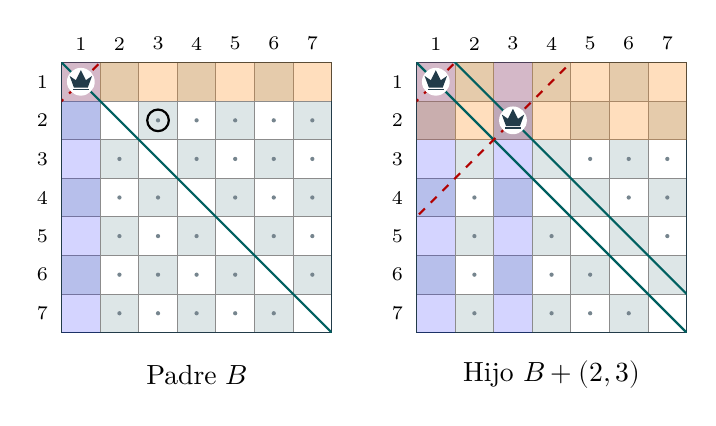
\begin{tikzpicture}[x=.49cm,y=.49cm]
 \foreach \etapa/\dx in {1/0,2/9.2}{
  \begin{scope}[shift={(\dx,0)}]
   \bcuadricula{7}
   \fill[orange,opacity=.26] (0,6) rectangle (7,7);
   \fill[blue,opacity=.17] (0,0) rectangle (1,7);
   \ifnum\etapa=2
    \fill[orange,opacity=.26] (0,5) rectangle (7,6);
    \fill[blue,opacity=.17] (2,0) rectangle (3,7);
   \fi
   \begin{scope}
    \clip (0,0) rectangle (7,7);
    \draw[teal!75!black,line width=.8pt] (.5,6.5) ++(-7,7) -- ++(14,-14);
    \draw[red!70!black,dashed,line width=.8pt] (.5,6.5) ++(-7,-7) -- ++(14,14);
    \ifnum\etapa=2
     \draw[teal!75!black,line width=.8pt] (2.5,5.5) ++(-7,7) -- ++(14,-14);
     \draw[red!70!black,dashed,line width=.8pt] (2.5,5.5) ++(-7,-7) -- ++(14,14);
    \fi
   \end{scope}
   \foreach \rr in {1,...,7}{
    \foreach \cc in {1,...,7}{
     \pgfmathtruncatemacro{\libre}{(\rr!=1)&&(\cc!=1)&&(abs(\rr-1)!=abs(\cc-1))}
     \ifnum\etapa=2
      \pgfmathtruncatemacro{\libre}{\libre&&(\rr!=2)&&(\cc!=3)&&(abs(\rr-2)!=abs(\cc-3))}
     \fi
     \ifnum\libre=1 \bmarca{7}{\rr}{\cc}\fi
    }
   }
   \breina{7}{1}{1}
   \ifnum\etapa=1
    \draw[black,line width=.8pt] (2.5,5.5) circle[radius=.28];
    \node at (3.5,-1.1) {Padre $B$};
   \else
    \breina{7}{2}{3}
    \node at (3.5,-1.1) {Hijo $B+(2,3)$};
   \fi
  \end{scope}
 }
\end{tikzpicture}
\caption{Una transición de un padre a un hijo en un tablero de orden siete. El padre tiene una reina
en la fila 1 y el hijo se obtiene al revelar la fila 2.
Las filas se numeran desde uno de arriba abajo y las columnas desde uno de izquierda a derecha.
Las coronas representan las reinas colocadas. Las bandas horizontales y verticales señalan sus filas y
columnas ocupadas. Las líneas continuas y discontinuas trazan las dos familias diagonales atacadas.
Cada punto indica una casilla disponible. En la fila siguiente, la $2$, las columnas $3,4,5,6,7$
tienen respectivamente $1,1,1,1,0$ completaciones, de modo que $Q(B)=4$. El círculo señala la elección
$(2,3)$ que produce el hijo de la derecha.}\label{fig:historia}
\end{figure}


\paragraph{Perfil y normalización.}
El Teorema~1.1 de~\cite{perfil} da el único perfil óptimo de masa uno, $\nu_1$, en el
cuadrado unidad. Denotamos su entropía por $s_1$ y escribimos $\Phi=s_1+1$. Como
en~\cite{perfil,ultimas,pred}, $m_D$ y $m_A$ son las proyecciones de $\nu_1$ sobre las dos familias
diagonales y $u_D=1-m_D$, $u_A=1-m_A$ sus vacancias. Si $f$ es una línea diagonal, $m_f$ y $u_f$
denotan los valores en $f$ de las funciones de su familia. Los Teoremas~1.2 y~1.3 y la Proposición~5.2
de~\cite{perfil} identifican los factores positivos y el límite en masa uno. El Teorema~7.7 del mismo
trabajo da el control hasta el extremo. Usamos la forma de~\cite[Sección~2]{pred},
\[
 \nu_1(r,c)=b_0 r_R(r)r_C(c)u_D(r-c)u_A(r+c),\qquad
 c_\nu\le\nu_1\le C_\nu,\quad \kappa_\nu\le u_D,u_A\le1.
\]
Las marginales de filas y columnas de $\nu_1$ valen uno, los factores son Lipschitz y $L_\nu$ denota
una constante de Lipschitz de $\nu_1$, como en~\cite{pred}. Las coordenadas continuas de la casilla
$(i,j)$ se toman en el centro de su celda de lado $1/n$.

\paragraph{Punto de Bethe y predictor.}
Escribimos RC por «filas y columnas». Como en~\cite{pred}, el \emph{punto de Bethe} de un residual
$B$ es el vector $p=(p_e)$, con un peso por casilla de $E(B)$, en el que se evalúa su predictor. Es
el punto estacionario de la entropía de Bethe
\begin{equation}\label{bethe}
 H_B(p)=-\sum_e p_e\log p_e+3\sum_e(1-p_e)\log(1-p_e)-\sum_fh_f\log h_f
\end{equation}
en el dominio $0<p_e<1/4$, $h_f>0$, con masas de fila y de columna iguales a uno. Aquí la
\emph{masa} de una diagonal $f$ es $\ell_f=\sum_{e\in f}p_e$ y su \emph{vacancia} es $h_f=1-\ell_f$.
La disponibilidad física es un indicador distinto de esta vacancia. En ese dominio $-H_B$ es
estrictamente convexa, de modo que hay a lo sumo un punto estacionario. Sólo usamos el punto de Bethe
en los tableros regulares de la Definición~\ref{def:regular} y en sus hijos, donde existe.

Cuando el grafo de filas y columnas del soporte es conexo, si $S_B$ es el operador de líneas, cuya
fórmula se da en la Sección~\ref{costes:normalizador}, y $\pdet$ es el producto de los autovalores
distintos de cero, el predictor satisface
\[
 L(B)=H_B(p)-\tfrac12\sum_e[\log(1-4p_e)-4\log(1-p_e)]
             -\tfrac12\log\pdet S_B+\tfrac12\log(4\pi k).
\]
El modo cero de $S_B$ es proporcional a $(\mathbf1_R,-\mathbf1_C,0)$; es el gauge de~\cite{pred}.
El cofactor de $S_B$ que se obtiene al suprimir la fila y la columna de una misma línea RC vale
$\pdet S_B/(2k)$, pues la componente correspondiente del vector unitario del modo cero tiene
cuadrado $1/(2k)$. Así, usar ese cofactor con $\tfrac12\log(2\pi)$, como
en~\cite[Secciones~6.1 y~7.1]{pred}, da el mismo $L(B)$.

El \emph{laplaciano de filas y columnas} de $p$ es, como en~\cite{pred}, el del grafo cuyos vértices
son las filas y las columnas vacías y en el que cada casilla disponible $e$ es una arista de peso
$p_e$ entre su fila y su columna. Su \emph{brecha} es su segundo autovalor más pequeño. Decimos que
$p$ cumple una \emph{cota de difusión} si $k\max_ep_e\le C$, una \emph{cota de vacancia} si
$h_f\ge\eta$ en toda diagonal y una \emph{cota de brecha} si esa brecha es al menos $\gamma$. Con
constantes $C,\eta,\gamma>0$ fijas, éstas son las cotas que piden los Teoremas~7.1 y~8.1
de~\cite{pred}: el primero para $k\ge\delta n$, y el segundo sin esa condición si la masa de cada
diagonal es a lo sumo un $\varepsilon$ pequeño.

Respecto de~\cite{pred} cambian algunas notaciones. Allí el hijo se escribe $B+c$, la fila se
sobreentiende en el cociente $\rho(B)$, que aquí es $\rho(B,i)$, y la masa y la vacancia de una
diagonal son $m_d$ y $h_d$; las demás diferencias se indican donde aparecen. Algunas letras, como $B$,
$E$, $J$, $S$, $T$ o $W$, designan en ciertas secciones objetos locales, que se definen donde aparecen;
por ejemplo, en la Sección~\ref{permanente} la letra $B$ denota la matriz $P-J_K$ y no un tablero.
Fuera del resumen y de la introducción, la letra $J$ no denota el operador de~\cite{pred}.

\paragraph{Leyes de revelado e inserción.}
Sorteamos uniformemente un orden $\sigma$ de las filas. Bajo la \emph{ley uniforme} $\mu$ elegimos,
de manera independiente de $\sigma$, una solución uniforme y revelamos sus reinas en ese orden.
Bajo la \emph{ley adaptativa} $\nu$, dada la siguiente fila $i$, elegimos $e$ con probabilidad
\[
 \nu_B(e\mid i)=\frac{\exp L(B+e)}{\sum_{e'\in R_i\cap E(B)}\exp L(B+e')},\qquad
 \rho(B,i)=\sum_{e'\in R_i\cap E(B)}\exp\{L(B+e')-L(B)\}.
\]
La \emph{ley auxiliar} $P^{\rm B}$ usa la misma fila uniforme y elige $e$ con probabilidad $p_e$. La
letra redonda de $P^{\rm B}$ y de su esperanza $\E_{\rm B}$ es de Bethe y no designa un tablero. Una
\emph{historia} es la sucesión de tableros $B_0,B_1,\dots$ que resulta, junto con el orden de las
filas. Decimos que un tablero con $k$ filas vacías tiene \emph{tamaño} $k$. En $B_t$ y en la historia
revelada $\mathcal F_t$, el índice $t$ cuenta inserciones. Al indexar por tamaño escribimos
$B^{(k)}=B_{n-k}$ y $\mathcal F^{(k)}=\mathcal F_{n-k}$. Esta última contiene las filas reveladas
hasta ese momento y sus casillas elegidas, antes de revelar la fila siguiente. En una historia
detenida, estos símbolos sólo se refieren a los niveles alcanzados.

\begin{definicion}[Tableros regulares y primera salida]\label{def:regular}
Fijamos $0<\delta<1$, $M=\lceil\delta n\rceil$ y un entero $K$ con $K_0\le K\le M$. El umbral $K_0$,
las constantes y las tolerancias que siguen se eligen en la Sección~\ref{meso:constantes}. Sea $B$ un
tablero de una historia, de tamaño $k$.
\begin{enumerate}[(a)]
\item \emph{Tramo macroscópico}, $k\ge M$. El tablero es \emph{regular} si la discrepancia $\Delta$
de la historia al llegar a él es menor que el radio $\varrho_{\rm mac}$ de la
Proposición~\ref{macro:parada}. La Sección~\ref{macro:observaciones} define esta discrepancia
con la partición $\mathcal I$, de paso $a_{\rm mac}$, de esa proposición.
\item \emph{Corte}, $k=M$. Se exige además que los observables de la
Sección~\ref{meso:regularidad} estén dentro de sus tolerancias de entrada y que
$D_{\max}(M)<\alpha M$, con la notación de la Sección~\ref{meso}.
\item \emph{Tramo mesoscópico}, $K\le k<M$. El tablero es regular si su punto de Bethe existe y
pertenece a la \emph{clase interior}: cumple las cotas de difusión, vacancia y brecha fijadas en la
Sección~\ref{meso:constantes} y la masa de cada diagonal es a lo sumo $\varepsilon$.
\end{enumerate}
La \emph{primera salida} de una historia es su primer tablero no regular, que llamamos \emph{tablero
de primera salida}. Su padre es regular. La historia se detiene en la primera salida o, si no la
hay, al llegar al tamaño $K$. El \emph{suceso de permanencia} $F$ consiste en que no haya salida:
todos los tableros hasta el de tamaño $K$, incluido éste, son regulares.
\end{definicion}
Para $n$ grande el tablero inicial es regular, pues su discrepancia es $O(1/n)$ (prueba de la
Proposición~\ref{macro:parada}). El punto de Bethe de un tablero regular cumple cotas de difusión,
vacancia y brecha con constantes fijas: en el tramo macroscópico por la Proposición~\ref{macro:maximo}
y el Corolario~\ref{macro:cambio}, y en el mesoscópico por definición. En el corte, las condiciones
adicionales lo sitúan ya en la clase interior, por la Proposición~\ref{meso:reconstruccion}. Sus
hijos, entre ellos el tablero de primera salida, heredan cotas del mismo tipo con constantes más
débiles, que llamamos \emph{cotas exteriores}; en el tramo mesoscópico, junto con una masa diagonal a
lo sumo $2\varepsilon$, definen la \emph{clase exterior}. En $\rho(B,i)$ intervienen todos los hijos
de $B$ en la fila $i$.

\begin{table}[htbp]\centering\small
\caption{Cómo se combinan las estimaciones en la comparación de los conteos.}
\begin{tabular}{@{}p{.31\linewidth}p{.59\linewidth}@{}}
\toprule Resultado & Estimaciones que utiliza \\ \midrule
Identidades \ref{hist:igualdad} y \ref{hist:inferior} & Partición por la siguiente fila y
normalización de las dos leyes.\\
Permanencia \ref{macro:cambio} & Balances \ref{macro:balances}, brecha \ref{macro:brecha},
reconstrucción \ref{macro:maximo} y parada \ref{macro:parada}.\\
Bandas \ref{prop:salida-banda-meso} & Prescripciones \eqref{prescr}, presupuesto
\ref{lema:presupuesto-meso}, concentración \ref{prop:concentracion-meso} y reconstrucción
\ref{meso:reconstruccion}.\\
Costes \ref{coste-macro} y \ref{coste-debil} & Comparación \ref{coste-comparacion} y, en el tramo
mesoscópico, normalizadores \ref{coste-normalizadores} y estimaciones del permanente
\ref{terminal-permanente} y \ref{terminal-normalizador}.\\
Último tablero \ref{terminal-error} & Geometría \ref{terminal-geometria}, pivotes
\ref{terminal-pivotes}, escalado \ref{terminal-escalado} y Proposición~3.1 de~\cite{dw}.\\
Teorema~\ref{princ} & Consistencia \ref{hist:consistencia}, cotas de salida y estimación
terminal bajo las dos leyes.\\ \bottomrule
\end{tabular}
\end{table}\begin{table}[!htbp]
\centering\small
\caption{Notación utilizada en la demostración.}
\label{tab:proof-notation}
\begin{tabular}{@{}p{.29\linewidth}>{\raggedright\arraybackslash}p{.65\linewidth}@{}}
\toprule
Símbolo & Significado \\
\midrule
$n,k$ & Orden del tablero inicial y número de filas vacías en el tablero residual. \\
$M,K$ & Corte $M=\lceil\delta n\rceil$ entre los dos tramos y tamaño terminal $K$. \\
$B_t,B^{(k)},B_\tau$ & Tablero tras $t$ inserciones, tablero con $k$ filas vacías
($B^{(k)}=B_{n-k}$) y tablero en la parada. \\
$\mathcal F_t,\mathcal F^{(k)}$ & Historia revelada, indexada por inserciones o por filas restantes,
con $\mathcal F^{(k)}=\mathcal F_{n-k}$. \\
\addlinespace[.22em]
$Q(B),L(B),g(B)$ & Conteo de completaciones, logaritmo del predictor y diferencia
$g(B)=\log Q(B)-L(B)$ cuando $Q(B)>0$. \\
$p_e,\ell_f,h_f$ & Peso de Bethe de la casilla $e$, masa de la diagonal $f$ y su vacancia
$h_f=1-\ell_f$. \\
\addlinespace[.22em]
$\mu,\nu,P^{\rm B}$ & Ley uniforme de revelado, ley adaptativa basada en el predictor
y ley auxiliar de Bethe. \\
$\tau,\rho(B,i),A_\tau$ & Tiempo de la primera salida o de la llegada al tamaño $K$, lo que ocurra
primero, cociente de normalización de la fila y logaritmo acumulado del cociente
$A_\tau=\sum_{t<\tau}\log\rho(B_t,i_t)$. \\
\addlinespace[.22em]
$F,G$ & Llegada al tamaño $K$ con regularidad hasta ese tablero inclusive, y subsuceso
$G=F\cap\{Q(B^{(K)})>0\}$. \\
$D_K$ & Suceso en el que dos cruces vacíos distintos en el tamaño $K$ comparten una diagonal. \\
\bottomrule
\end{tabular}
\end{table}


\section{Las dos comparaciones sobre historias detenidas}\label{historias}
Sea $\tau$ una parada que usa solamente el orden de filas y lo revelado hasta el paso actual.
Supongamos que cada padre anterior a la parada y cada uno de sus hijos tienen un predictor finito.
Escribimos $B_t$ para el tablero de la historia tras $t$ inserciones e $i_t$ para la fila que se
revela a continuación. Escribimos $\omega$ para el prefijo de casillas, incluyendo la última
inserción, $B_\tau$ para su residual y $\mu^\tau,\nu^\tau$ para las leyes conjuntas del orden y del
prefijo. Definimos
\[
 A_\tau=\sum_{t<\tau}\log\rho(B_t,i_t),\qquad g(B)=\log Q(B)-L(B)\quad(Q(B)>0).
\]

\begin{lema}[Comparación en la primera parada]\label{hist:igualdad}
Si $Q(B_0)>0$, se tiene $\mu^\tau\ll\nu^\tau$ y
\begin{equation}\label{super}
 g(B_0)=\E_\mu[A_\tau+g(B_\tau)]-D(\mu^\tau\Vert\nu^\tau).
\end{equation}
Aquí $D$ es la entropía relativa de las dos leyes discretas.
\end{lema}
\begin{proof}
Fijado el orden $\sigma$, cada una de las $Q(B_\tau)$ completaciones prolonga el prefijo de
una sola manera. Bajo $\nu$ multiplicamos las probabilidades de escoger las sucesivas casillas.
Las diferencias de los predictores se suman telescópicamente. Así, las masas en el mismo átomo son
\[
 \mu^\tau(\sigma,\omega)=\frac{Q(B_\tau)}{n!\,Q(B_0)},\qquad
 \nu^\tau(\sigma,\omega)=\frac{\exp\{L(B_\tau)-L(B_0)-A_\tau\}}{n!}.
\]
La segunda masa es positiva en el soporte de la primera. Tomar el logaritmo de su cociente
en el orden $\mu^\tau/\nu^\tau$ da $A_\tau+g(B_\tau)-g(B_0)$. Su media bajo $\mu^\tau$
es, por definición, la entropía relativa que figura en \eqref{super}.
\end{proof}

\begin{proposicion}[Cota inferior por permanencia]\label{hist:inferior}
Sea $\tau$ la parada de la Definición~\ref{def:regular}: la primera salida o, si no la hay, la
llegada al tamaño $K$. Sea $F$ el suceso de permanencia. En $F$ se tiene $B^{(K)}=B_\tau$.
Sea $G$ el conjunto de las historias de $F$ con $Q(B^{(K)})>0$. Si $s=\nu(G)>0$, entonces
\begin{equation}\label{infer}
 g(B_0)\ge \E_{\nu(\cdot\mid G)}[A_\tau+g(B^{(K)})]+\log s.
\end{equation}
\end{proposicion}
\begin{proof}
Para cada orden, los prefijos detenidos distintos tienen conjuntos disjuntos de completaciones.
En cada historia de $G$, multiplicar su masa bajo $\nu^\tau$ por $\exp\{A_\tau+g(B^{(K)})\}$
deja $Q(B^{(K)})e^{-L(B_0)}/n!$. Sumando primero en los prefijos y después en los órdenes obtenemos
\[
 \int_G\exp\{A_\tau+g(B^{(K)})\}\,d\nu^\tau\le Q(B_0)e^{-L(B_0)} .
\]
La integral es $s$ veces la esperanza condicional del exponencial. La concavidad del logaritmo
da \eqref{infer}, también cuando el condicionamiento modifica la distribución del orden.
\end{proof}

\begin{corolario}[Consistencia acumulada]\label{hist:consistencia}
En cada padre anterior a la parada supongamos las hipótesis del Teorema~7.1 y del Corolario~7.2
de~\cite{pred} para $k>M=\lceil\delta n\rceil$, y las del Teorema~8.1 del mismo trabajo para
$K<k\le M$. Entonces $|A_\tau|\le C/K+O_\delta(n^{-1})$ uniformemente en las historias.
\end{corolario}
\begin{proof}
Esos resultados dan $|\log\rho(B,i)|\le C_*/k^2$ en cada fila, incluyendo en $\rho$ todos los
hijos de esa fila. Para los padres con $k>M$ la constante depende de $\delta$ y de las cotas de
difusión, vacancia y brecha. Para los padres con $K<k\le M$ depende de las constantes de la clase
débil de~\cite[Sección~8.1]{pred}. En este rango, un padre regular de la Definición~\ref{def:regular}
está en la clase interior, por definición si $k<M$ y por la Proposición~\ref{meso:reconstruccion}
si $k=M$. La suma de $k^{-2}$ para $k>m$ es a lo sumo $\int_m^\infty t^{-2}\,dt=1/m$.
Una historia que termina antes usa un
subconjunto de estos sumandos.
\end{proof}

\section{Permanencia cuando quedan al menos \texorpdfstring{$\delta n$}{δn} filas}\label{macro}

\subsection{Proceso de revelado y trayectoria de comparación}

Fijamos $0<\delta<1$. Tras $s$ elecciones escribimos $k=n-s$, $x=k/n$ y $t=s/n$. Bajo $P^{\rm B}$ se
revela la permutación uniforme $\sigma$ de las filas una a una. Condicionalmente a la historia
$\mathcal F_s$ de las elecciones y de las filas ya reveladas, la próxima fila es uniforme entre las
$k$ filas vacías. Si $p$ es el punto de Bethe del tablero actual, la probabilidad condicional de
seleccionar una
casilla $e$ es $p_e/k$. En las casillas fuera del soporte ponemos $p_e=0$. Los índices discretos van de
$1$ a $n$. Los centros físicos
$r_i=(i-\tfrac12)/n$ y $c_j=(j-\tfrac12)/n$ sitúan la diagonal $D(e)=i-j$ en $r_i-c_j$ y la
antidiagonal $A(e)=i+j-1$ en $r_i+c_j$. Denotamos por $X_f$ el indicador de disponibilidad de una
línea y por $Y_e=\prod_{f\ni e}X_f$ el de una casilla. Como en la Sección~\ref{leyes}, $\ell_f$ y
$h_f$ son la masa y la vacancia de una diagonal o antidiagonal $f$ en el punto $p$.

\begin{lema}[Pérdida de una casilla]\label{macro:casilla}
La probabilidad condicional de ocupar una fila o columna disponible es $1/k$. La probabilidad de
ocupar una diagonal disponible $f$ es $\ell_f/k$. Para $e=(i,j)$ se tiene
\[
 \E_{\rm B}[Y_e(s+1)-Y_e(s)\mid\mathcal F_s]
 =-\frac{Y_e(s)}{k}\bigl(2+\ell_{D(e)}+\ell_{A(e)}-3p_e\bigr).
\]
\end{lema}
\begin{proof}
Las dos primeras fórmulas se obtienen sumando $p_e/k$ sobre la línea correspondiente. Si $Y_e=1$, las
cuatro líneas que pasan por $e$ sólo se cortan en esa casilla. En la suma de sus masas $e$ aparece
cuatro veces y hay que contarla una vez. Si $Y_e=0$, ninguna elección puede volver a hacerla
disponible.
\end{proof}

En el cuadrado unidad usamos el perfil
\[
 \nu_1(r,c)=b_0r_R(r)r_C(c)u_D(r-c)u_A(r+c).
\]
Sus marginales de filas y columnas valen uno. Para $d\in[-1,1]$ y $a'\in[0,2]$, sus proyecciones
sobre las dos familias diagonales, es decir, las masas de sus fibras, son
\[
 m_D(d)=\int_{\{0\le r,r-d\le1\}}\nu_1(r,r-d)\,dr,\qquad
 m_A(a')=\int_{\{0\le r,a'-r\le1\}}\nu_1(r,a'-r)\,dr .
\]
Aquí y en adelante la notación bajo el signo de integral exige que ambas coordenadas pertenezcan a
$[0,1]$. Las vacancias son $u_f=1-m_f$. Usamos $c_\nu\le\nu_1\le C_\nu$, $u_f\ge\kappa_\nu>0$ y la
regularidad Lipschitz del perfil lleno \cite[Teoremas~1.1--1.3, Proposición~5.2 y
Teorema~7.7]{perfil}. Las masas de las fibras son Lipschitz en su parámetro. En efecto, desplazarlo en
$\epsilon$ mueve los extremos de integración a lo sumo en $|\epsilon|$ cada uno y cambia el integrando
en la parte común a lo sumo en $L_\nu|\epsilon|$.

La proposición siguiente reúne los objetivos deterministas con los que comparamos el proceso cuando
queda una fracción $x$ de filas. Para una diagonal $f$, $U_f(x)$ es el objetivo de su indicador de
disponibilidad y $\ell_f^*(x)$ el de su masa. En un punto $(r,c)$, $J_x$ es el objetivo del indicador
de disponibilidad de la casilla y $v_x/n$ el del peso de Bethe de una casilla disponible.

\begin{proposicion}[Trayectoria de comparación]\label{macro:trayectoria}
Para una línea diagonal $f$, un punto $(r,c)$ y $0\le x\le1$, escribimos
\begin{gather*}
 U_f(x)=u_f+xm_f,\qquad \ell_f^*(x)=\frac{xm_f}{U_f(x)},\\
 J_x=x^2U_D(x)U_A(x),\qquad
 W_x=\frac{\nu_1}{U_D(x)U_A(x)}.
\end{gather*}
Los subíndices $D,A$ sin argumento se evalúan en $r-c,r+c$, respectivamente. Como $u_f\ge\kappa_\nu$,
$W_x$ se prolonga por continuidad hasta $W_0=\nu_1/(u_Du_A)=b_0r_Rr_C$, el peso usado en la
Sección~\ref{meso:regularidad}. Se tiene $J_1=1$. Para $0<x\le1$, ponemos $v_x=W_x/x$. Entonces
$J_xv_x=x\nu_1$, ambas marginales de $J_xv_x$ valen $x$ y
\begin{equation}\label{macro:derivadas}
 \partial_t U_f=-\frac{\ell_f^*}{x}U_f,\qquad
 \partial_t\log J_x=-\frac{2+\ell_D^*+\ell_A^*}{x},\qquad
 1-\ell_f^*=\frac{u_f}{U_f}\ge\kappa_\nu .
\end{equation}
En particular,
\[
 v_x=\frac{b_0}{x}\,r_Rr_C\frac{u_D}{U_D}\frac{u_A}{U_A},
 \qquad xv_x\le C_\nu/\kappa_\nu^2 .
\]
\end{proposicion}
\begin{proof}
Se tiene $U_f(1)=1$, $\kappa_\nu\le U_f(x)\le1$ y $dx/dt=-1$. Por tanto $\partial_t U_f=-m_f$. Derivar
el producto que define $J_x$ da la segunda identidad de \eqref{macro:derivadas}. La fórmula de $v_x$
se obtiene sustituyendo la factorización de $\nu_1$. La identidad del producto y las afirmaciones
sobre las marginales siguen por integración.
\end{proof}

La comparación que sigue necesita los productos de disponibilidades de varias líneas. Las
observaciones de las dos familias diagonales por separado sólo dan las medias de cada factor.
Definimos a continuación sumas de productos y demostramos su concentración sin imponer independencia a
las líneas.

\subsection{Observaciones en intervalos, fibras y rectángulos}\label{macro:observaciones}

Tomamos una partición $\mathcal I$ de $[0,1]$ en intervalos de longitud a lo sumo $a_{\rm mac}$, con
extremos
asignados a un solo intervalo. Podemos usar intervalos iguales. Un índice pertenece al intervalo de su
centro físico. Para filas y columnas registramos
\[
 N^R_I=\frac1n\sum_{r_i\in I}X_{R_i},\qquad
 N^C_I=\frac1n\sum_{c_j\in I}X_{C_j},\qquad
 N^{R,*}_I=N^{C,*}_I=x|I|.
\]
En una fila el parámetro de la fibra es $c$. En una columna, diagonal o antidiagonal es $r$. Fijamos
una línea $\lambda$, que llamamos \emph{distinguida}: es la línea cuya fibra se observa. Dado un
intervalo $I$, escribimos $\lambda_I$ para la parte de la fibra física cuyo parámetro pertenece a
$I$, y $dz$ para la medida de ese parámetro. No aparece un factor de
longitud euclídea en las fibras oblicuas, pues hay $n$ índices por unidad de $r$.

\begin{definicion}[Observaciones por fibra]\label{macro:fibras}
Mientras $\lambda$ está disponible, su observación es
\[
 F_{\lambda,I}=\frac1n\sum_{e\in\lambda_I}
                  \prod_{f\ni e,\ f\ne\lambda}X_f .
\]
En cada una de las cuatro familias el objetivo $F^*_{\lambda,I}$ es la integral en $\lambda_I$ de la
densidad de la segunda columna de la tabla. La última columna da la suma de tasas de las tres líneas
que figuran en el producto, antes de dividir por $x$.
\[
\begin{array}{c|c|c}
 \lambda & \text{densidad del objetivo} & H^*_{\lambda}(e)\\ \hline
 R_i & xU_DU_A  & 1+\ell_D^*+\ell_A^*\\
 C_j & xU_DU_A  & 1+\ell_D^*+\ell_A^*\\
 D_d & x^2U_A   & 2+\ell_A^*\\
 A_{a'} & x^2U_D & 2+\ell_D^*
\end{array}
\]
Si la elección del paso ocupa $\lambda$, se conservan los valores de $F_{\lambda,I}$ y
$F^*_{\lambda,I}$ inmediatamente anteriores al paso y se mantienen constantes en adelante. Llamamos
a esto \emph{regla de congelación}. Los balances del Lema~\ref{macro:balances} sólo utilizan líneas
todavía disponibles.
\end{definicion}

Para un rectángulo ordenamos sus posiciones como
$e_1=(i,j)$, $e_2=(i',j)$, $e_3=(i',j')$, $e_4=(i,j')$.
Llamamos ordinaria a la cuádrupla $(i,i',j,j')$ si $i\ne i'$, $j\ne j'$ y las cuatro etiquetas de cada
familia diagonal son distintas entre sí. Las demás cuádruplas son $O(n^3)$. Cada igualdad prohibida es
una ecuación lineal no idéntica en cuatro índices. Fijar tres índices apropiados determina el cuarto,
y sólo hay un número fijo de igualdades. Esta estimación también cubre los bordes del tablero.

\begin{definicion}[Observaciones de rectángulos]\label{macro:rectangulos}
Para $T\subseteq\{1,2,3,4\}$ y una caja $\Theta\in\mathcal I^4$, se siguen la suma y su objetivo
\begin{align*}
 P_{\Theta,T}&=\frac1{n^4}
 \sum_{(i,i',j,j')\in\Theta}^{\rm ord}
 X_{R_i}X_{R_{i'}}X_{C_j}X_{C_{j'}}
 \prod_{m\in T}X_{D(e_m)}X_{A(e_m)},\\
 P^*_{\Theta,T}&=\int_\Theta x^4\prod_{m\in T}U_{D(e_m)}U_{A(e_m)}
                  \,dr\,dr'\,dc\,dc'.
\end{align*}
Las posiciones en la integral se forman con las cuatro coordenadas continuas. El patrón de
$T=\varnothing$ cuenta sólo las dos filas y las dos columnas. Los rectángulos individuales que pierden
una línea dejan de contribuir.
\end{definicion}

Medimos las discrepancias por
\begin{align*}
 \Delta_0&=\sum_{I\in\mathcal I}
   (\bigl|N^R_I-x|I|\bigr|+\bigl|N^C_I-x|I|\bigr|),\\
 \Delta_F&=\max_{\lambda}\sum_{I\in\mathcal I}|F_{\lambda,I}-F^*_{\lambda,I}|,\\
 \Delta_R&=\sum_{\Theta\in\mathcal I^4}\ \sum_{T\subseteq\{1,2,3,4\}}
                      |P_{\Theta,T}-P^*_{\Theta,T}|,\qquad
 \Delta=\Delta_0+\Delta_F+\Delta_R .
\end{align*}
En la primera línea, $x|I|$ es la masa objetivo de cada intervalo. Escribimos $C_{\mathcal I}$ para
constantes
que pueden depender de la partición fija $\mathcal I$ y
\[
 \zeta=\Delta_0+\Delta_F+a_{\rm mac}+C_{\mathcal I}/n .
\]
En las $k$ filas y $k$ columnas disponibles consideramos
\[
 q_{ij}=\frac{Y_{ij}\nu_1(r_i,c_j)}{kU_{D(i,j)}U_{A(i,j)}},\qquad
 V_{ij}=\frac{\nu_1(r_i,c_j)}k .
\]
Los factores $U$ se evalúan en $x$, de modo que $q_{ij}=Y_{ij}W_x(r_i,c_j)/k=Y_{ij}v_x(r_i,c_j)/n$.
La matriz $q$ es el candidato explícito al punto de Bethe: la Proposición~\ref{macro:maximo} prueba
que $p_e/q_e$ está cerca de uno en las casillas disponibles. La matriz $V$ se obtiene de $q$ al
sustituir $Y_{ij}$ por $U_DU_A$, que es su objetivo cuando la fila y la columna están disponibles.

La Figura~\ref{fig:rectangulo} muestra dos posiciones elegidas y el signo que les corresponde.
\begin{figure}[htbp]
\centering
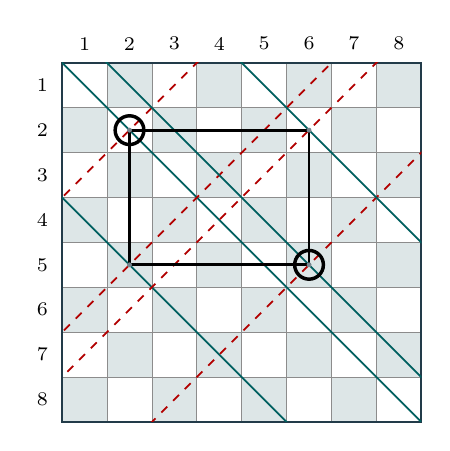
\begin{tikzpicture}[x=.57cm,y=.57cm]
 \bcuadricula{8}
 \begin{scope}
  \clip (0,0) rectangle (8,8);
  \foreach \rr/\cc in {2/2,5/2,5/6,2/6}{
   \draw[teal!75!black,line width=.65pt] ({\cc-.5},{8.5-\rr}) ++(-8,8) -- ++(16,-16);
   \draw[red!70!black,dashed,line width=.65pt] ({\cc-.5},{8.5-\rr}) ++(-8,-8) -- ++(16,16);
  }
 \end{scope}
 \draw[black,line width=1pt] (1.5,6.5) rectangle (5.5,3.5);
 \foreach \rr/\cc in {2/2,5/2,5/6,2/6}{\bmarca{8}{\rr}{\cc}}
 \draw[black,line width=1.25pt] (1.5,6.5) circle[radius=.32];
 \draw[black,line width=1.25pt] (5.5,3.5) circle[radius=.32];
\end{tikzpicture}
\caption{Rectángulo en un tablero vacío de orden ocho. Las filas se numeran desde uno de arriba abajo
y las columnas desde uno de izquierda a derecha. Los vértices en orden son $e_1=(2,2)$, $e_2=(5,2)$,
$e_3=(5,6)$ y $e_4=(2,6)$. Pasan por ellos cuatro diagonales $i-j$ (continuas) y cuatro antidiagonales
$i+j-1$ (discontinuas). Los círculos eligen los vértices opuestos $e_1,e_3$. El término de la
expansión con $T=\{1,3\}$ tiene signo $(-1)^{4-2}=+1$.}\label{fig:rectangulo}
\end{figure}


\begin{lema}[Balances por intervalos y fibras]\label{macro:balances}
Para $k\ge\delta n$, las sumas por filas y por columnas de $V$ difieren de uno en
$O_\delta(\Delta_0+a_{\rm mac}+C_{\mathcal I}/n)$. Las de $q$ difieren de uno y sus masas sobre líneas
diagonales
disponibles difieren de $\ell_f^*$ en
$O_\delta(\Delta_F+a_{\rm mac}+C_{\mathcal I}/n)$, uniformemente en las líneas.
\end{lema}
\begin{proof}
En cada intervalo sustituimos el peso por su valor en un punto de la parte física que se integra. Los
pesos $\nu_1$ y $W_x=\nu_1/(U_DU_A)$ son uniformemente acotados y Lipschitz. El error de la sustitución,
sumado sobre los intervalos de una línea, es $O_\delta(a_{\rm mac})$, pues multiplica la suma de masas
de esa
línea. El error de las masas ponderadas es a lo sumo la norma suprema del peso por la suma de
discrepancias absolutas. La conversión de $1/n$ a $1/k$ aporta $1/x$. Para $V$ el objetivo de una fila
es $x^{-1}\int\nu_1(r,c)x\,dc=1$, y análogamente en las columnas. En una fila disponible, los tres
indicadores del observable de fibra dan $Y_{ij}$ y su masa ponderada objetivo es
\[
 \frac1x\int_0^1 \frac{\nu_1}{U_DU_A}\,xU_DU_A\,dc=1.
\]
La misma cuenta con $dr$ da la suma de una columna. Para la diagonal $d$ el objetivo es
\[
 \frac1x\int_{D_d}\frac{\nu_1}{U_DU_A}\,x^2U_A\,dr
 =\frac{xm_D(d)}{U_D(d)} .
\]
En una antidiagonal se intercambian $D$ y $A$ y resulta $xm_A/U_A$. Las aproximaciones de extremos o
por sumas de Riemann en la partición fija cuestan a lo sumo $C_{\mathcal I}/n$.
\end{proof}

\begin{lema}[Cancelación de los dieciséis términos y brecha]\label{macro:brecha}
Para $E=q-V$ se tiene
\[
 \|E\|_{\rm op}\le C_\delta(\Delta_R+a_{\rm mac}+C_{\mathcal I}/n)^{1/4}.
\]
Si $\Delta$, $a_{\rm mac}$ y $C_{\mathcal I}/n$ son suficientemente pequeños en función de $\delta$ y
del perfil, el
laplaciano de filas y columnas con pesos $q$ tiene brecha al menos $c_\nu/2$ en el complemento del
vector constante.
\end{lema}
\begin{proof}
Por los valores singulares y la expansión de la traza,
\[
 \|E\|_{\rm op}^4\le {\rm tr}((EE^T)^2)
 =\sum_{i,i',j,j'}E_{ij}E_{i'j}E_{i'j'}E_{ij'} .
\]
En el sumando se puede extraer el indicador de las cuatro líneas de filas y columnas disponibles y el
factor $k^{-4}\prod_m\nu_1(e_m)$. Lo que resta es $\prod_{m=1}^4(B_m-1)$, con

\[ B_m=\frac{X_{D(e_m)}X_{A(e_m)}}{U_{D(e_m)}U_{A(e_m)}}. \]
Si $B_T=\prod_{m\in T}B_m$ y en los subíndices
abreviamos los conjuntos por sus elementos, la expansión completa es
\[
 \begin{aligned}
 1
 &-(B_1+B_2+B_3+B_4)\\
 &+(B_{12}+B_{13}+B_{14}+B_{23}+B_{24}+B_{34})\\
 &-(B_{123}+B_{124}+B_{134}+B_{234})+B_{1234}.
 \end{aligned}
\]
Las cuádruplas excepcionales aportan $O_\delta(1/n)$ en total, pues cada producto es
$O_\delta(k^{-4})$. Para cada término ordinario, el peso que multiplica el patrón de la
Definición~\ref{macro:rectangulos} en la suma normalizada por $n^4$ es
\[
 W_T=x^{-4}\frac{\prod_m\nu_1(e_m)}
                 {\prod_{m\in T}U_{D(e_m)}U_{A(e_m)}} .
\]
Tiene norma suprema y constante Lipschitz acotadas en función de $\delta$ y el perfil. En cada caja,
sustituirlo por una constante cuesta en conjunto $O_\delta(a_{\rm mac})$, porque para cada $T$ la masa
de todas
las cajas suma a lo sumo uno. Sustituir después las masas discretas por sus objetivos cuesta
$O_\delta(\Delta_R)$. Al devolver el peso variable a la integral, la densidad objetivo ponderada de
cada uno de los dieciséis términos es exactamente $\prod_m\nu_1(e_m)$. Por tanto su coeficiente total
es $1-4+6-4+1=0$. Esto prueba la estimación de la norma.

Sea $V'=V-c_\nu\mathbf1\mathbf1^T/k$. Sus entradas son no negativas y sus sumas de filas y columnas son
a lo sumo $1-c_\nu+O_\delta(\zeta)$ por el Lema~\ref{macro:balances}. La cota de Schur da el mismo
límite para $\|V'\|_{\rm op}$. Si $(u,v)\perp\mathbf1_{2k}$, entonces $(\sum_i u_i)(\sum_j
v_j)=-(\sum_i u_i)^2\le0$. En la forma cuadrática del laplaciano el término de la matriz constante es,
pues, no negativo. Los grados diagonales son $1+O_\delta(\zeta)$, y
$2\|u\|_2\|v\|_2\le\|u\|_2^2+\|v\|_2^2$. La forma cuadrática queda acotada inferiormente por
\[
 \bigl(c_\nu-O_\delta(\zeta)-\|E\|_{\rm op}\bigr)
                   (\|u\|_2^2+\|v\|_2^2).
\]
Reduciendo los tres umbrales se obtiene la brecha afirmada. La potencia de exponente $1/4$ se usa sólo
para garantizar esta brecha.
\end{proof}

\subsection{Reconstrucción del punto de Bethe}\label{macro:reconstruccion}
En toda esta subsección suponemos $k\ge\delta n$, como en el Lema~\ref{macro:balances}.

\begin{proposicion}[Reequilibrado de filas y columnas]\label{macro:reequilibrado}
Bajo los umbrales del Lema~\ref{macro:brecha}, existe una matriz $\bar p$ con el soporte de $q$,
sumas por filas y por columnas exactamente iguales a uno y
\[
 \max_{q_e>0}\left|\frac{\bar p_e}{q_e}-1\right|\le C_\delta\zeta .
\]
Sus vacancias diagonales son al menos $\kappa_\nu/2$, sus entradas son $O_\delta(1/k)$ y su laplaciano
de filas y columnas conserva una brecha positiva uniforme.
\end{proposicion}
\begin{proof}
Restringimos las variables a las casillas disponibles, donde $q_e>0$. Sea $B$ la matriz de incidencia
de filas y columnas por casillas; como en~\cite[Sección~6.1]{pred}, la letra $B$ designa aquí esa
matriz y no un tablero. Sea $J$ la matriz diagonal que cambia el signo de las coordenadas de
columnas, y pongamos $B_o=JB$. Para $b=\mathbf1-Bq$ se tiene $\|b\|_\infty=O_\delta(\zeta)$ y
$\mathbf1^TJb=0$, pues la suma de las masas por filas coincide con la suma por columnas. Con el
laplaciano de filas y columnas $L_q$ de pesos $q$, definimos
\[
 L_q=B_o\operatorname{diag}(q)B_o^T,\qquad
 \phi=L_q^+Jb,\qquad z=\operatorname{diag}(q)B_o^T\phi .
\]
La brecha y la compatibilidad dan $Bz=b$ y $\|\phi\|_2\le C_\delta\sqrt{k}\,\zeta$. En un vértice
$\gamma$ del grafo, es decir, en una fila o una columna, la ecuación $L_q\phi=Jb$ y su grado
$d_\gamma=1+O_\delta(\zeta)$ dan
\[
 d_\gamma|\phi_\gamma|\le |b_\gamma|+
 \left(\sum_{e\in\gamma}q_e^2\right)^{1/2}\|\phi\|_2,
 \qquad \sum_{e\in\gamma}q_e^2\le \frac{C_\delta}{k}d_\gamma .
\]
Así $\|\phi\|_\infty=O_\delta(\zeta)$ y $|z_e|/q_e\le2\|\phi\|_\infty$. Tomamos $\bar p=q+z$. La
comparación multiplicativa de pesos conserva una fracción fija de la brecha de $L_q$. También cambia
cada masa diagonal en $O_\delta(\zeta)$ por el Lema~\ref{macro:balances}. Las vacancias objetivo son
al menos $\kappa_\nu$ por \eqref{macro:derivadas}, lo que da las cotas de la proposición al reducir
los umbrales.
\end{proof}

\begin{lema}[Inversa tangente en el punto factible]\label{macro:inversa}
Para $\bar p$ como en la Proposición~\ref{macro:reequilibrado}, denotemos por $K_{\bar p}$ la hessiana
negativa de la entropía de Bethe en $\bar p$ y por $Z$ una matriz de columnas ortonormales que
generan $\ker B$. Para $n$
grande,
\[
 R=Z(Z^TK_{\bar p}Z)^{-1}Z^T,\qquad
 \|\operatorname{diag}(\bar p)^{-1}R\|_{\infty\to\infty}\le C_\delta .
\]
\end{lema}
\begin{proof}
Damos el argumento matricial de \cite[Secciones~6.3, 6.4 y~7.2]{pred} en este punto factible. Sea $D$ la
incidencia de casillas por diagonales de las dos familias, como en~\cite[Sección~6.1]{pred}; la
letra $D$ sola designa esa matriz y $D(e)$ sigue siendo la diagonal de la casilla $e$. Sean
$H=\operatorname{diag}(h_f(\bar p))$ y
\[
 w_e=\left(\frac1{\bar p_e}-\frac3{1-\bar p_e}\right)^{-1},
 \qquad W=\operatorname{diag}(w_e),\qquad
 K_{\bar p}=W^{-1}+DH^{-1}D^T .
\]
Se tiene $w_e/\bar p_e=1+O_\delta(1/k)>0$. Si $\Upsilon$ se forma apilando $B_o$ y $D^T$, el
sistema para $v=R\psi$ equivale a
\begin{equation}\label{macro:sistema-inverso}
 (\Upsilon W\Upsilon^T+\operatorname{diag}(0,H))\,y=\Upsilon W\psi,\qquad
 v=W(\psi-\Upsilon^Ty).
\end{equation}
En efecto, el primer bloque da $B_ov=0$ y el segundo $D^Tv=Hy_D$, donde $y_D$ reúne las dos familias
diagonales. De aquí $K_{\bar p}v=\psi-B_o^Ty_{RC}$.

Resolvemos \eqref{macro:sistema-inverso} con $y_{RC}\perp\mathbf1_{2k}$, condición compatible con el
primer bloque. La forma cuadrática de la matriz del sistema es
\[
 \|W^{1/2}(B_o^Ty_{RC}+Dy_D)\|_2^2+y_D^THy_D .
\]
Su segundo término domina $\kappa_\nu\|y_D\|_2^2/2$. Además
$\|W^{1/2}Dy_D\|_2^2\le 2\max_f\sum_{e\in f}w_e\,\|y_D\|_2^2$,
pues cada casilla incide en dos diagonales. La brecha de $B_oWB_o^T$ y la desigualdad triangular
muestran entonces que la forma también domina una constante positiva por $\|y_{RC}\|_2^2$. Los
coeficientes de $\Upsilon W\psi$ están acotados por $C_\delta\|\psi\|_\infty$ y hay a lo sumo $2k+4n$
líneas. Por coercividad,
$\|y\|_2\le C_\delta\sqrt{k}\|\psi\|_\infty$.

Cada diagonal principal del sistema está separada de cero por las sumas de filas y columnas o por
$H$. Dos líneas distintas se cortan a lo sumo en una casilla. Así, fuera de la diagonal principal,
cada coeficiente tiene módulo a lo sumo $\max_e w_e=O_\delta(1/k)$, y en cada fila la suma de módulos
es a lo sumo tres veces el grado ponderado de la línea, que es $O_\delta(1)$. La norma euclídea de la
parte no diagonal de cada fila es, por tanto, $O_\delta(k^{-1/2})$. Aplicando la ecuación coordenada a
coordenada resulta $\|y\|_\infty\le C_\delta\|\psi\|_\infty$. Como $\Upsilon^Ty$ suma cuatro
multiplicadores con signo, la segunda fórmula de \eqref{macro:sistema-inverso} da la estimación anunciada.
\end{proof}

\begin{proposicion}[Punto estacionario y máximo único]\label{macro:maximo}
Existen umbrales positivos para $\Delta$, $a_{\rm mac}$, $C_{\mathcal I}/n$ y un $n$ mínimo,
dependientes de $\delta$ y del
perfil, tales que el punto de Bethe $p$ del tablero existe y es el máximo global único de la entropía
de Bethe entre los puntos factibles. Llamamos \emph{factible} a todo $s=(s_e)$, con una coordenada
por casilla disponible, tal que $s_e\ge0$, las sumas de fila y de columna valen uno y $h_f(s)\ge0$
en toda diagonal. El punto $p$ cumple
\begin{equation}\label{macro:predictor}
 \max_{q_e>0}|p_e/q_e-1|\le C_\delta(\zeta+k^{-1}),\qquad
 \max_{f\ {\rm diagonal\ disponible}}|\ell_f(p)-\ell_f^*|
                       \le C_\delta(\zeta+k^{-1}).
\end{equation}
La segunda cota incluye las dos familias diagonales.
\end{proposicion}
\begin{proof}
Escribamos el negativo del gradiente, módulo multiplicadores de fila y de columna, como
\[
 \Xi_e(p)=\log p_e+3\log(1-p_e)-\log h_{D(e)}(p)-\log h_{A(e)}(p).
\]
En $q$, al usar las vacancias objetivo, se obtiene exactamente
\[
 \log q_e-\log(u_D/U_D)-\log(u_A/U_A)
 =\log(b_0/k)+\log r_R(r_i)+\log r_C(c_j).
\]
Al pasar a $\bar p$, las diferencias de los logaritmos de vacancias son $O_\delta(\zeta)$ y
$3\log(1-\bar p_e)=O_\delta(k^{-1})$. Además
$\log(\bar p_e/q_e)=(B_o^T\phi)_e+O_\delta(\zeta^2)$.
Sustrayendo los multiplicadores exhibidos obtenemos un representante $\psi$ de $\Xi(\bar p)$, módulo
multiplicadores, con $\|\psi\|_\infty\le C_\delta(\zeta+k^{-1})$.

Usamos la norma $\|v\|_{\rm rel}=\max_e|v_e|/\bar p_e$. En $\|v\|_{\rm rel}\le\vartheta$ tenemos
$|(D^Tv)_f|\le\vartheta\ell_f(\bar p)\le\vartheta$. Para $\vartheta$ pequeño, las casillas siguen
positivas y las
vacancias superan $\kappa_\nu/4$. Las fórmulas de Taylor para los tres tipos de logaritmos dan
\[
 \Xi(\bar p+v)=\Xi(\bar p)+K_{\bar p}v+N(v),\qquad
 \|N(v)\|_\infty\le C_\delta\vartheta^2,\qquad
 \|N(v)-N(w)\|_\infty\le C_\delta\vartheta\|v-w\|_{\rm rel}.
\]
Para $\log p_e$ se aplica el desarrollo a $v_e/\bar p_e$. Para $\log(1-p_e)$ y los logaritmos de las
vacancias, los denominadores están separados de cero y las respectivas perturbaciones están acotadas
por $\vartheta$. La ecuación de estacionariedad en $\ker B$ es $v=-R(\psi+N(v))$. Por el
Lema~\ref{macro:inversa}, esta aplicación preserva la bola de radio $2C_\delta\|\psi\|_\infty$ y tiene
constante de contracción menor que $1/2$ al reducir los umbrales. Su punto fijo $p=\bar p+v$ es
factible y estacionario. La comparación con $q$ y el Lema~\ref{macro:balances} dan
\eqref{macro:predictor}.

Para seleccionar el máximo global, sea $d(a,b)=a\log(a/b)-a+b$, extendida por continuidad a $a=0$.
Para cualquier competidor factible $s$, restamos en la entropía su término lineal en $p$. Este término
se anula por estacionariedad y por la igualdad de las sumas de filas y columnas. La diferencia de
entropías entre $s$ y $p$
vale
\[
 -\sum_e\bigl[d(s_e,p_e)-3d(1-s_e,1-p_e)\bigr]
 -\sum_f d(h_f(s),h_f(p)).
\]
Para $0<b\le e^{-4}$, la función $\tilde d_b(a)=d(a,b)-3d(1-a,1-b)$ satisface
\[
 \tilde d_b(b)=\tilde d_b'(b)=0,\qquad
 \tilde d_b''(a)=\frac{1-4a}{a(1-a)},\qquad
 \tilde d_b(1)=\log(1/b)-4+4b>0 .
\]
Es estrictamente convexa hasta $1/4$ y, por consiguiente, positiva allí salvo en $b$. En $[1/4,1]$ la
concavidad la sitúa por encima de la cuerda entre dos valores positivos. Para $n$ grande,
$p_e=O_\delta(1/k)\le e^{-4}$. Toda casilla en que $s_e\ne p_e$ da una pérdida estricta y cada
divergencia de vacancia es no negativa. Así $p$ es el único máximo.
\end{proof}

\subsection{Deriva por familia y control hasta la primera salida}\label{macro:control}

\begin{lema}[Pérdida condicional de un patrón]\label{macro:deriva}
Supongamos que el padre cumple los umbrales de la Proposición~\ref{macro:maximo} y que $k\ge\delta n$.
Para un conjunto $\mathcal L$ de un número acotado de líneas distintas disponibles, sea $H^*(\mathcal
L)$ la suma de un uno por fila o columna y de $\ell_f^*$ por cada diagonal o antidiagonal $f$. En un
paso,
\[
 P^{\rm B}(\text{se ocupa alguna línea de }\mathcal L\mid\mathcal F_s)
 =\frac{H^*(\mathcal L)}{k}
       +O_\delta\!\left(\frac{\zeta+k^{-1}}{k}\right).
\]
Las tasas de las fibras son las de la Definición~\ref{macro:fibras}, y la del término rectangular $T$
es
\[
 H_T^*=4+\sum_{m\in T}\bigl(\ell_{D(e_m)}^*+\ell_{A(e_m)}^*\bigr).
\]
\end{lema}
\begin{proof}
La suma de probabilidades individuales se obtiene con el Lema~\ref{macro:casilla}. Al sustituir las
masas diagonales por sus objetivos se comete el error de \eqref{macro:predictor} dividido por $k$ y
multiplicado por el número de líneas. Cada intersección de dos líneas distintas tiene probabilidad a
lo sumo $\max_e p_e/k=O_\delta(k^{-2})$. Las dos primeras desigualdades de inclusión y exclusión
acotan el error de la unión por la suma de esas intersecciones.

Para una línea distinguida disponible $\lambda$, escribimos $Y_{e|\lambda}=\prod_{f\ni
e,\,f\ne\lambda}X_f$. Si $Y_{e|\lambda}=1$, su contribución disminuye cuando se alcanza alguna de las
otras tres líneas sin ocupar $\lambda$. Excluir la ocupación simultánea de $\lambda$ y de una de las
tres líneas cambia la probabilidad en $O_\delta(k^{-2})$. Si se ocupa $\lambda$, la regla de
congelación conserva el observable. Por tanto, con $\nabla_s$ denotando el incremento de un paso,
\[
 \E_{\rm B}[\nabla_s F_{\lambda,I}\mid\mathcal F_s]
 =-\frac1{kn}\sum_{e\in\lambda_I}Y_{e|\lambda}H_\lambda^*(e)
   +O_\delta\!\left(\frac{\zeta+k^{-1}}{k}F_{\lambda,I}\right).
\]
La derivada temporal de cada densidad de fibra en la tabla es $-H^*_\lambda/x$ veces esa densidad, por
\eqref{macro:derivadas}. El incremento de su objetivo sin congelación es la integral de esta derivada
dividida por $n$, con error de Taylor $O_\delta(n^{-2}|\lambda_I|)$, donde $|\lambda_I|$ mide el
intervalo de su parámetro. La probabilidad de congelación es $O(1/k)$ y el incremento ordinario del
objetivo es $O_\delta(|\lambda_I|/n)$. Congelar el objetivo en el paso en que se ocupa la línea añade
por tanto
$O_\delta(|\lambda_I|/(kn))$ a su deriva condicional. Una fibra ya congelada tiene ambas derivas
iguales a cero.

Para las masas de filas o columnas se tiene exactamente
$\E_{\rm B}[\nabla_s N_I\mid\mathcal F_s]=-N_I/k$ y el objetivo disminuye en $|I|/n$. Para el
rectángulo se aplica la fórmula de la unión a las cuatro líneas de filas y columnas y las $2|T|$
líneas diagonales. Son distintas para las cuádruplas ordinarias. Si $Y_{T}$ denota el producto de sus
indicadores,
\[
 \E_{\rm B}[\nabla_s P_{\Theta,T}\mid\mathcal F_s]
 =-\frac1{kn^4}\sum_{(i,i',j,j')\in\Theta}^{\rm ord}Y_T H_T^*
   +O_\delta\!\left(\frac{\zeta+k^{-1}}{k}P_{\Theta,T}\right).
\]
Cuando $Y_T=0$ su contribución sigue valiendo cero. La densidad del objetivo tiene derivada
exactamente igual a $-H_T^*/x$ veces ella misma. La segunda derivada temporal está uniformemente
acotada para $x\ge\delta$, de modo que el error de Taylor integrado es $O_\delta(|\Theta|/n^2)$.
\end{proof}

\begin{proposicion}[Cota de parada bajo la ley auxiliar]\label{macro:parada}
Sea $M=\lceil\delta n\rceil$. Para todo radio $\varrho_{\rm mac}>0$ suficientemente pequeño, se
puede fijar una partición $\mathcal I$ de paso $a_{\rm mac}$ y constantes
$c_{\delta,\varrho_{\rm mac}},C_{\delta,\varrho_{\rm mac}}>0$ de modo que, para $n$ suficientemente
grande,
\[
 P^{\rm B}\!\left(\max_{0\le s\le n-M}\Delta(s)\ge\varrho_{\rm mac}\right)
 \le C_{\delta,\varrho_{\rm mac}}\exp(-c_{\delta,\varrho_{\rm mac}}n).
\]
Se puede imponer el mismo control a una partición de observación fija pasando a un refinamiento suyo.
\end{proposicion}
\begin{proof}
Sea $\tau$ el primer índice con $\Delta(s)\ge\varrho_{\rm mac}$, limitado por $n-M$. Paramos en
$\tau$ las discrepancias y los incrementos centrados de cada observable menos su objetivo. El
incremento que llega a $\tau$ se incluye si la historia hasta el padre seguía dentro del radio
$\varrho_{\rm mac}$. Sea $\mathcal M^*$ la suma de los máximos temporales absolutos de esas
martingalas para intervalos de filas y columnas y para cajas y subconjuntos, más el máximo sobre las
líneas distinguidas de la suma de los máximos absolutos de sus intervalos.

En una caja o intervalo restamos en la deriva empírica y en la del objetivo un mismo valor de la tasa
$H^*$, tomado en un punto de esa región. El término de tasa constante es a lo sumo $C_\delta/n$ veces
la discrepancia absoluta de masa en esa región. La oscilación de $H^*$ es $O_\delta(a_{\rm mac})$ por
regularidad espacial y multiplica la suma de la masa empírica y la masa objetivo. En todas las
subfibras de una línea esas masas suman a lo sumo dos. Para cada uno de los dieciséis tipos, también
suman a lo sumo dos sobre todas las cajas. En los errores de Taylor las longitudes o volúmenes suman a
lo sumo uno por familia o tipo. Estos hechos dan, con una constante $C_\delta$ independiente del
número de intervalos,
\begin{equation}\label{macro:gronwall}
 \Delta(s\wedge\tau)\le \Delta(0)+\mathcal M^*
 +\frac{C_\delta}{n}\sum_{j<s\wedge\tau}\Delta(j)
 +C_\delta(a_{\rm mac}+C_{\mathcal I}/n),\qquad 0\le s\le n-M .
\end{equation}
Para las fibras primero se suman los errores absolutos sobre sus intervalos y luego se toma el máximo
sobre las líneas. La contribución de cada fibra cesa desde su congelación. Las estimaciones del
Lema~\ref{macro:deriva} sólo emplean en la deriva $\zeta$, que es lineal en $\Delta_0+\Delta_F$. El
exponente $1/4$ del Lema~\ref{macro:brecha} no afecta al coeficiente de \eqref{macro:gronwall}.

Hay $O_{\mathcal I}(n)$ martingalas escalares. Para una fibra que sigue disponible cada línea recién
ocupada afecta a lo sumo una casilla de la fibra, pues las líneas distintas se cortan a lo sumo una
vez. En el paso que ocupa la línea distinguida se congela toda su observación. Para un rectángulo,
requerir que una de las líneas ocupadas pase por una posición fija del rectángulo determina una
relación lineal no idéntica y permite $O(n^3)$ cuádruplas. Cada incremento de una masa normalizada,
incluido el del objetivo, tiene por tanto módulo a lo sumo $C_\delta/n$. La misma cota, con otra
constante, vale después de centrar y parar los incrementos.

Si $(\xi_j)$ son diferencias de martingala con $|\xi_j|\le d_j$, para $\theta>0$ la convexidad de la
exponencial entre $-d_j$ y $d_j$ y la media condicional cero dan
$\E[\exp(\theta\xi_j)\mid\mathcal F_{j-1}]\le\cosh(\theta d_j)\le\exp(\theta^2d_j^2/2)$. El producto
compensado es una supermartingala positiva. Pararla en el primer $h$ con $\sum_{j\le h}\xi_j\ge u$,
aplicar la misma cuenta a $-\xi_j$ y optimizar $\theta$ da
\begin{equation}\label{macro:max-mart}
 P\left(\max_{h\le m}\left|\sum_{j\le h}\xi_j\right|\ge u\right)
 \le 2\exp\!\left(-\frac{u^2}{2\sum_{j\le m}d_j^2}\right).
\end{equation}
Para la partición $\mathcal I$ fija existe $C'_{\mathcal I}$ tal que si todas las martingalas escalares
tienen máximo absoluto menor
que $b/C'_{\mathcal I}$ entonces $\mathcal M^*<b$. El factor $C'_{\mathcal I}$ cuenta los intervalos de
una sola fibra y las
observaciones de intervalos y rectángulos. El número de líneas distinguidas sólo interviene en la
unión de sucesos. De \eqref{macro:max-mart} resulta
\[
 P^{\rm B}(\mathcal M^*\ge b)\le C_{\mathcal I}(n+1)\exp(-c_{\delta,\mathcal I}b^2 n).
\]

Al inicio $x=U_f=1$. Las sumas de retícula por intervalos y cajas, la aproximación de los extremos
de las fibras y las $O(n^3)$ cuádruplas excepcionales dan $\Delta(0)\le C_{\mathcal I}/n$,
uniformemente en la línea distinguida. Elegimos primero $\varrho_{\rm mac}$ dentro de los umbrales
deterministas, después $a_{\rm mac}$ y $b$ con
$e^{C_\delta}(b+C_\delta a_{\rm mac})<\varrho_{\rm mac}/3$, y finalmente $n$ grande a partición
fija. Gronwall discreto en \eqref{macro:gronwall} da $\Delta(s\wedge\tau)<\varrho_{\rm mac}$ siempre
que $\mathcal M^*<b$, también para el paso que llega a $\tau$. Esto excluye la primera salida y
prueba la cota, absorbiendo $n+1$ en la exponencial. Al refinar una partición todas las masas y
objetivos de una región gruesa se obtienen sumando los de las regiones finas, también para fibras
congeladas. La desigualdad triangular transfiere la cota a la partición gruesa.
\end{proof}

\begin{corolario}[Cambio de ley hasta la primera salida]\label{macro:cambio}
La conclusión de la Proposición~\ref{macro:parada} vale bajo la ley $\nu$ con otras constantes
$C_{\delta,\varrho_{\rm mac}},c_{\delta,\varrho_{\rm mac}}>0$. En particular, con probabilidad al menos
$1-C_{\delta,\varrho_{\rm mac}}\exp(-c_{\delta,\varrho_{\rm mac}}n)$, en todos los tableros hasta $k=M$,
incluido ese
extremo, el punto de
Bethe es el máximo único y cumple cotas macroscópicas uniformes de difusión, vacancia y brecha.
\end{corolario}
\begin{proof}
Por \eqref{macro:predictor}, eligiendo los umbrales suficientemente pequeños se pueden fijar, por
ejemplo, una cota superior $4C_\nu/\kappa_\nu^2$ para $k\max_e p_e$, una cota inferior $\kappa_\nu/4$
para las vacancias y una cota inferior estrictamente menor que $c_\nu/8$ para la brecha. La
comparación de pesos en el Lema~\ref{macro:brecha} y la Proposición~\ref{macro:reequilibrado}
justifica esta última elección. Éstas son las cotas macroscópicas que se verifican en cada padre
regular del tramo macroscópico.

Para dicho padre y cualquiera de sus hijos, la expansión de un paso de \cite[Teorema~7.1 y
Corolario~7.2, con sus pruebas]{pred} da
\[
 L(B+e)-L(B)=\log[p_e(1+d_e)]+r_e,\qquad
 |d_e|\le C'_\delta/k,\qquad |r_e|\le C''_\delta/k^2,\qquad
 \sum_{e\in i}p_ed_e=0
\]
en cada fila disponible $i$. Aquí $d_e$ es la corrección relativa $\delta_c$
de~\cite[Teorema~7.1]{pred} y $r_e$ es el resto $r_c$ de su prueba. La construcción del hijo por
eliminación en \cite[Sección~6.5]{pred} permite usar la expansión también en el tablero de primera
salida. Sólo
se exige el control del padre. Las dos leyes usan la misma elección uniforme de la próxima fila.
Condicionalmente a esa fila, el cociente de la probabilidad de columna bajo $\nu$ y su probabilidad
$p_e$ bajo $P^{\rm B}$ es
\[
 \frac{(1+d_e)e^{r_e}}{\sum_{e'\in i}p_{e'}(1+d_{e'})e^{r_{e'}}} .
\]
Para $k\ge2C'_\delta$ todos los factores $1+d_{e'}$ son positivos. La cancelación por fila implica
$\sum_{e'\in i}p_{e'}(1+d_{e'})=1$, de modo que el denominador pertenece a
$[e^{-C''_\delta/k^2},e^{C''_\delta/k^2}]$. El módulo del logaritmo del cociente es a lo sumo
$2C'_\delta/k+2C''_\delta/k^2$.

A lo largo de una trayectoria parada en la primera salida o al llegar a $M$, el módulo del logaritmo
de la densidad relativa se acota por \[
\sum_{k=M+1}^{n}\left(\frac{2C'_\delta}{k}+\frac{2C''_\delta}{k^2}\right) \le
2C'_\delta\log(n/M)+2C''_\delta/M=O_\delta(1). \] La cota incluye la transición que produce la
salida. Al sumar sobre las historias paradas en las que la discrepancia alcanza el radio
$\varrho_{\rm mac}$ obtenemos, por la Proposición~\ref{macro:parada}, la cola exponencial afirmada.
Fuera de ese suceso se aplica la reconstrucción determinista en todos los tableros hasta $M$.
\end{proof}

\section{Permanencia desde el corte hasta un número fijo de filas}\label{meso}
En esta sección indexamos por el tamaño: $\mathcal F_k$ es la historia hasta el tablero de tamaño $k$,
mientras que en la Sección~\ref{macro} el índice de $\mathcal F_s$ era el número de pasos. Sea
$M=\lceil\delta n\rceil$. En el tablero de tamaño $k$ escribimos $D_{\max}(k)$ para el máximo, sobre
las diagonales de las dos familias del tablero inicial, del número de cruces vacíos que
contiene la línea, disponibles o no. Esta cantidad es
decreciente a lo largo de la historia y domina la cuenta de casillas disponibles en cualquier
diagonal de las dos familias. Todas las probabilidades de esta sección corresponden a la ley
adaptativa $\nu$ iniciada en el tablero inicial. Denotamos por $G_k^-$ el suceso de que, al llegar al
tamaño $k$, todos los tableros de tamaños estrictamente mayores hayan sido regulares
(Definición~\ref{def:regular}). Incluimos en $G_k^-$ la transición que llega al tablero de primera
salida.

\subsection{Prescripciones y presupuesto diagonal}
\begin{lema}[Cotas de un paso]\label{meso:paso}
En un padre regular de tamaño $k$, sea $\nu_B(j\mid i)$ la probabilidad adaptativa de elegir la
columna $j$ dada la elección de la fila $i$, con $\nu_B(j\mid i)=0$ en las casillas no disponibles.
Existen constantes $C_q,C_{\rm c}$, que se pueden fijar antes de $\delta$ y de la cota $\varepsilon$
de la masa diagonal, tales que, para $n$ suficientemente grande y $k$ mayor que un umbral fijo,
\begin{align*}
 \nu(i\text{ elegida}\mid\mathcal F_k)&=1/k,\\
 \left|\nu(j\text{ elegida}\mid\mathcal F_k)-1/k\right|&\le C_{\rm c}/k^2,\\
 \nu((i,j)\text{ elegida}\mid\mathcal F_k)&\le C_q/k^2 .
\end{align*}
\end{lema}
\begin{proof}
En la representación por hijo de \cite[Teoremas~7.1 y~8.1]{pred}, la perturbación relativa
de $p_e$ es $d_e+O(k^{-2})$, con $d_e=O(k^{-1})$ y $B(p\odot d)=0$ por \cite[Sección~6.1]{pred},
donde $B$ designa aquí la matriz de incidencia de filas y columnas y no el tablero. Al
normalizar por la fila se conserva el resto relativo $O(k^{-2})$ porque $\sum_jp_{ij}d_{ij}=0$. Al
sumar por la columna también desaparece la parte lineal, pues $\sum_i p_{ij}d_{ij}=0$. Así $\sum_i
\nu_B(j\mid i)=1+O(k^{-2})$. En el tramo macroscópico, el resto de la probabilidad de elegir la
columna es $O_\delta(k^{-3})$. Para cada $\delta$ fijado, $k\ge\delta n$ permite absorberlo en
$k^{-2}$ con coeficiente uno tomando $n$ grande. En el mismo tramo, $\nu_B(j\mid i)\le 2p_{ij}$ para
$n$ grande y la constante de difusión de $p$ proviene del perfil. En el tramo mesoscópico se usan las
cotas de difusión, vacancia y brecha de la clase exterior, cuyas constantes no dependen de $\delta$
ni de $\varepsilon$. La representación requiere que el padre sea regular y las estimaciones por hijo de la
prueba del teorema citado, también para el tablero de primera salida.
\end{proof}

\begin{lema}[Filas y columnas prescritas]\label{meso:prescripciones}
Para cualesquiera $s$ filas y $t$ columnas fijas del tablero inicial se cumple
\begin{equation}\label{prescr}
 \nu(\text{las $s$ filas y $t$ columnas siguen vacías en el tamaño $m$},G_m^-)
 \le (m/n)^{s+t}\exp\{C(st+s+t)/m\}.
\end{equation}
Si no caben las prescripciones, el miembro izquierdo es cero. La constante $C$ es común a todos los
valores de $s,t$.
\end{lema}
\begin{proof}
En un padre regular de tamaño $k$ que contiene los índices prescritos, el Lema~\ref{meso:paso} da que
la probabilidad de elegir una fila prescrita es $s/k$, la de elegir una columna prescrita es al menos
$t/k-C_{\rm c}t/k^2$, y la intersección es a lo sumo $C_qst/k^2$. Dentro de cada familia los sucesos
son disjuntos. El factor de supervivencia es por tanto a lo sumo
$\exp[-(s+t)/k+C_1(st+s+t)/k^2]$. Iteramos desde $n$ hasta $m+1$, descartando las historias que ya
tenían un padre no regular. Las desigualdades $\sum_{k=m+1}^n k^{-1}\ge\log(n/m)-1/m$ y
$\sum_{k=m+1}^n k^{-2}\le1/m$ dan \eqref{prescr}, también cuando $s,t$ dependen de $m$.
\end{proof}

Fijar $s$ casillas de una diagonal prescribe exactamente $s$ filas y $s$ columnas distintas,
independientemente de la disponibilidad. Hay menos de $4n$ diagonales y cada una admite a lo sumo
$\binom ns$ elecciones. Por \eqref{prescr} y $\binom ns\le(en/s)^s$,
existe $C_{\rm geo}<\infty$ fijo tal que, para $1\le s\le m/4$,
\begin{equation}\label{geompres}
 \nu(D_{\max}(m)\ge s,G_m^-)\le 4n\left(\frac{C_{\rm geo}m^2}{ns}\right)^s .
\end{equation}
En efecto, el factor $\exp[C(s^2+2s)/m]$ se absorbe en una constante elevada a $s$. Para $s>m$ el
suceso es vacío.

Llamamos \emph{suelo} al tamaño $K$ hasta el que se sigue la historia, y \emph{presupuesto diagonal}
a la suma del lema siguiente, que controla el efecto acumulado de las diagonales sobre las derivas.
\begin{lema}[Presupuesto diagonal]\label{lema:presupuesto-meso}
Fijemos $A\ge4C_{\rm geo}$ y $\chi>0$ pequeña. Para cualquier suelo entero $K_0\le K\le M$, salvo un
suceso de probabilidad $\le C_\chi e^{-c_\chi K}$, hasta el tablero de primera salida inclusive se
tiene
\[
 \sum_{\substack{K<k\le M\\\text{padres regulares alcanzados}}}
          \frac{(D_{\max}(k)-1)_+}{k^2}
 \le C\{A(\delta+1/n)+\chi+1/K\}.
\]
Aquí basta que $A(\delta+1/n)+\chi+1/K<1/4$. Además, fijado $0<\alpha_{\rm geo}<1/4$, para cualquier tasa
$\lambda>0$ se puede tomar $\delta>0$ tan pequeño y luego $K_0,n$ tan grandes que
\begin{gather*}
 \nu\big(\exists\,K\le k\le M:\ G_k^-,\ D_{\max}(k)\ge\alpha_{\rm geo} k\big)
 \le C_\lambda e^{-\lambda K},\\
 \nu(G_M^-,D_{\max}(M)\ge\alpha_{\rm geo} M)\le C_\lambda e^{-\lambda M}.
\end{gather*}
\end{lema}
\begin{proof}
Tomamos los extremos superiores $m$ de los intervalos $[2^jK,\min(2^{j+1}K,M)]$ no vacíos, incluyendo
$M$ en el último, y en cada uno fijamos $s_m=\lceil Am^2/n+\chi\sqrt{Km}\rceil$. Se cumple
$s_m/m\le1/4$ y $v=C_{\rm geo}m^2/(ns_m)\le1/4$. La cota
$4nv^{s_m}=4C_{\rm geo}m^2v^{s_m-1}/s_m\le C m^2e^{-c s_m}$
elimina el factor $n$ del tablero inicial. Sumando sobre los extremos se obtiene
$C_\chi e^{-c_\chi K}$: también la suma sobre todos los enteros $m\ge K$ de
$m^2e^{-c\chi\sqrt{Km}}$ tiene esa cota,
separando las bandas $2^jK\le m<2^{j+1}K$. En un intervalo alcanzado por una historia todavía regular,
su extremo superior ya fue alcanzado sin salida previa. Allí $D_{\max}(m)<s_m$ fuera de la excepción.
La monotonía y $s_m-1\le Am^2/n+\chi\sqrt{Km}$ acotan la contribución del intervalo por
$C(Am/n+\chi\sqrt{K/m})$. Sumamos las dos progresiones geométricas, incluida la última banda
truncada.

Para la segunda estimación ponemos $s=\lceil\alpha_{\rm geo} k\rceil\le k/4$ en \eqref{geompres}.
Ahora $v\le
2C_{\rm geo}\delta/\alpha_{\rm geo}$ para $n$ grande y $4nv^s\le4C_{\rm geo} k^2v^{s-1}/s$. Escogemos
$\alpha_{\rm geo}\log(\alpha_{\rm geo}/(2C_{\rm geo}\delta))>\lambda$ con desigualdad estricta. La
diferencia absorbe el
factor polinómico
y la suma sobre $k\ge K$, aumentando $K_0$ si hace falta. La estimación en $M$ usa únicamente el
término $k=M$.
\end{proof}

\subsection{Patrones y fibras con línea distinguida disponible}
Un patrón fijo $H$ tiene $s$ índices de fila, $t$ de columna, un conjunto $S$ de posiciones que deben
ser casillas disponibles y un peso determinista $w$ de norma acotada en cada asignación de índices.
Los indicadores de intervalos pueden incorporarse a $w$. Sea $Z_H$ la suma sobre asignaciones
inyectivas por familia, con sus pesos e indicadores de disponibilidad, dividida por $(k)_s(k)_t$,
donde $(k)_s=k(k-1)\cdots(k-s+1)$. Tomamos $K_0$ mayor que el doble de todos los órdenes de patrones
usados.
\begin{lema}[Incrementos de un patrón]\label{lema:incrementos-meso}
Para un padre regular de tamaño $k$ y $\Delta Z_H=Z_H(k-1)-Z_H(k)$,
\[
 |\mathbb E_\nu(\Delta Z_H\mid\mathcal F^{(k)})|
 \le C_H\frac{1+(D_{\max}(k)-1)_+}{k^2},\qquad
 |\Delta Z_H|\le C_H/k .
\]
Las mismas cotas valen para $F_i(k)/k$, donde $i$ es una fila distinguida y $F_i(k)=\sum_{j\ {\rm
disponible}}Y_{ij}w_{ij}$, si el paso se condiciona a que sobreviva $i$. También valen para una
columna distinguida condicionada a sobrevivir. Aquí $Y_{ij}$ es el indicador de disponibilidad de la
casilla; los pesos son fijos y acotados.
\end{lema}
\begin{proof}
La probabilidad de que el borrado de fila y columna afecte una asignación fija es
$(s+t)/k+O_H(k^{-2})$ por inclusión-exclusión y el Lema~\ref{meso:paso}. El cociente exacto de las
normalizaciones es $(1-s/k)(1-t/k)$. Se cancela pues el término de primer orden de la deriva. Después
de descontar el borrado por fila y columna, para perder una casilla $e\in S$ aún disponible hay que
elegir otra casilla en una de sus dos diagonales. En cada diagonal hay a lo sumo $(D_{\max}(k)-1)_+$
posibilidades y cada una tiene probabilidad $\le C_q/k^2$. Sumamos sobre $S$ y sobre las asignaciones,
usando el valor absoluto del peso. Para el salto, el borrado de una fila y una columna afecta
$O_H(k^{s+t-1})$ asignaciones. Cuando $S\ne\varnothing$, las dos diagonales borradas contienen a lo
sumo $2k$ cruces vacíos y cada casilla fijada en una posición de $S$ afecta a lo sumo
$O_H(k^{s+t-2})$ asignaciones. El cambio de la normalización es relativo $O_H(1/k)$. No se impone
restricción de diagonal distinta a las posiciones de un patrón.

Condicionemos ahora sólo el siguiente paso a que sobreviva $i$. La probabilidad de borrar una columna
$j$ es
\[
 \frac{\nu(j\ {\rm elegida}\mid\mathcal F^{(k)})-
       \nu((i,j)\ {\rm elegida}\mid\mathcal F^{(k)})}{1-1/k}
   =1/k+O(k^{-2})
\]
uniformemente. Para una columna distinguida se intercambian familias y el denominador es
$1-1/k+O(k^{-2})$. En ambos casos la pérdida esperada por el borrado transversal es $F_i/k+O(1/k)$,
pues hay a lo sumo $k$ sumandos acotados. Tras dividir por $k-1$ se cancela con el cambio de
normalización, con error $O(k^{-2})$. Para cada casilla de la fibra, la probabilidad adicional de
perderla por una diagonal es a lo sumo $2C_q(D_{\max}(k)-1)_+/k^2$ dividido por la probabilidad de
supervivencia de la línea
distinguida en este paso, uniformemente separada de cero. Sumamos sobre la fibra y dividimos por
$k-1$. Cada diagonal corta la fibra en a lo sumo una casilla, por lo que el salto normalizado es
$O(1/k)$.
\end{proof}

\begin{proposicion}[Concentración de los observables]\label{prop:concentracion-meso}
Para una familia fija de patrones y tipos de fibras de pesos acotados, fijemos $b_1>0$ y $\chi>0$.
Existe $c_{\rm pat}>0$ tal que, para cada suelo $K$, en las historias de entrada regular, salvo
probabilidad $\le C e^{-c_{\rm pat}K}$, cada observable alcanzado antes de la primera salida o en la
transición que
llega a ella difiere de su valor en $M$ en a lo sumo
\[
 C_H\{A(\delta+1/n)+\chi+1/K\}+b_1 .
\]
Para las fibras se compara cada línea distinguida todavía disponible con su propia fibra en $M$. La
tasa depende de las constantes de la clase exterior, de la familia de observables, de $b_1$ y de
$\chi$.
\end{proposicion}
\begin{proof}
Restamos a cada incremento su esperanza predecible y congelamos el proceso a partir del tablero de
primera salida. Para un patrón sin línea distinguida, el salto centrado en el paso desde el tamaño
$u$ es a lo sumo $2C_H/u$. La desigualdad maximal de Azuma \eqref{macro:max-mart}, con
$\sum_{u>k}u^{-2}\le1/k$, acota por $2\exp(-c_H b_1^2k)$ la probabilidad de que la martingala alcance
en módulo $b_1$ desde $M$ hasta $k$. El
Lema~\ref{lema:presupuesto-meso} y la suma de $u^{-2}$ acotan la deriva acumulada en todos los
prefijos a la vez.

Fijada la historia de entrada y una de sus líneas distinguidas, usemos el núcleo auxiliar que en cada
padre regular divide el núcleo original restringido a los hijos que mantienen disponible la línea
distinguida por su probabilidad de supervivencia $y_u$. Este núcleo sólo condiciona el paso siguiente.
En cualquier prefijo que llega con la línea distinguida disponible al tamaño $k$, incluido el que
termina en la primera salida, el peso bajo $\nu$ es el peso auxiliar multiplicado por
\[
 \prod_{u=k+1}^{M}y_u
 =\prod_{u=k+1}^{M}\big(1-1/u+O(u^{-2})\big)
 =(k/M)\exp(O(1/k)).
\]
Para la fila el producto es exactamente $k/M$. Para la columna el error es uniforme aun cuando los
factores dependan de los tableros del prefijo. La misma identidad de pesos vale en un instante de
parada porque se aplica por separado a cada prefijo terminal. Bajo el núcleo auxiliar restamos la
deriva condicional del Lema~\ref{lema:incrementos-meso} y congelamos al llegar al tablero de primera
salida. La
misma desigualdad maximal de Azuma vale desde cualquier historia de entrada regular.

En la banda $m\le k<2m$, con $m=2^jK$, paremos en la primera observación de la banda en que la martingala
de esta línea distinguida tenga módulo $\ge b_1$, si existe. Al transferir los prefijos de parada a
$\nu$, el factor cuesta a lo sumo $(2m/M)e^{C/m}$. La unión condicional sobre las $M$ líneas
distinguidas de cada familia y los tipos fijos de pesos, y después la suma sobre las bandas, cuestan a
lo sumo $\sum_m C m e^{-c_H b_1^2 m}\le C'e^{-c' b_1^2K}$. Mientras la línea distinguida siga disponible,
la resta de deriva en estas trayectorias es exactamente la del núcleo auxiliar; su módulo acumulado
queda controlado por el presupuesto en la trayectoria original. El fallo del presupuesto se cuenta una
sola vez bajo $\nu$, mediante el Lema~\ref{lema:presupuesto-meso}, después de integrar sobre la
historia de entrada. Así no aparece un factor $M$ en la cola de ese fallo ni un factor $n$ en la cola
de las fibras.
\end{proof}

\subsection{Reconstrucción de las condiciones de regularidad}\label{meso:regularidad}
Escribimos $W_0=\nu_1/(u_Du_A)=b_0r_Rr_C$, que es el valor en $x=0$ del peso $W_x$ de la
Proposición~\ref{macro:trayectoria}, $q_{ij}=Y_{ij}W_{0,ij}/k$ y
$V_{ij}=\nu_{1,ij}/k$, evaluados en las coordenadas originales de la casilla. Las cotas $c_\nu,C_\nu$
para la densidad, la vacancia mínima $\kappa_\nu$ y la constante de Lipschitz $L_\nu$ son las
constantes fijas del perfil. Consideramos una partición fija de $[0,1]$ en intervalos de longitud a
lo sumo $a_{\rm mes}$. El radio $\varrho_{\rm mac}$ y el paso $a_{\rm mac}$ de la
Sección~\ref{macro} se eligen después, en el punto~5 de la Sección~\ref{meso:constantes}, en función
de esta partición, de las tolerancias que siguen y de $\delta$ (Lema~\ref{meso:entrada}). Para filas
y columnas controlamos sus proporciones restantes en cada intervalo con objetivo la longitud del
intervalo. Fijamos una tolerancia $\varrho_{\rm mes}>0$ y tolerancias individuales cuya suma es a lo
sumo $\varrho_{\rm mes}$ por familia, por ejemplo $\varrho_{\rm mes}|I|$ para $I$ en esta partición.
Las fibras de fila y columna tienen pesos $W_0$, objetivo $1$ y tolerancia a lo sumo
$\varrho_{\rm mes}$ cada una.

Para describir los otros patrones escribamos $T=\{1,2\}\times\{1,2\}$. Por cada $S\subseteq T$ tomamos
el patrón de dos filas y dos columnas que requiere una casilla disponible en las posiciones de $S$. Su
peso es $\prod_{e\in S}W_{0,e}\prod_{e\in T\setminus S}\nu_{1,e}$. Los dieciséis tienen un mismo
objetivo,
\[
 \int_{[0,1]^4}\nu_1(r,c)\nu_1(r,c')\nu_1(r',c)\nu_1(r',c')\,dr\,dr'\,dc\,dc' .
\]
La normalización inyectiva es $(k)_2^2$. Usar $k^4$ y agregar las asignaciones que repiten fila o
columna modifica cada patrón en $O(1/k)$, porque hay $O(k^3)$ asignaciones adicionales con peso
acotado. Con $E=q-V$, como en el Lema~\ref{macro:brecha}, la identidad
\[
 \operatorname{tr}\big[(EE^{T})^2\big]
 =\sum_{i,i',j,j'} E_{ij}E_{i'j}E_{i'j'}E_{ij'}
\]
produce los dieciséis términos así extendidos con signos $(-1)^{4-|S|}$. Los dieciséis objetivos se
cancelan por $(1-1)^4=0$. Se escogen las tolerancias positivas por separado de modo que su suma, más
$O(1/K_0)$, sea menor que la cuarta potencia de la cota espectral requerida. Entonces $\|q-V\|_{\rm
op}\le\operatorname{tr}[(EE^T)^2]^{1/4}$ es menor que dicha cota. La expansión incluye
$S=\varnothing$, y permite diagonales repetidas en todos los términos.

\begin{proposicion}[Reconstrucción de la clase interior]\label{meso:reconstruccion}
Existen constantes $C_{\rm int},\eta_{\rm int},\gamma_{\rm int}>0$, que dependen sólo del perfil, con
la propiedad siguiente.
Supongamos que los observables de esta sección, es decir, las proporciones por intervalos, las fibras
y los dieciséis términos del rectángulo, están dentro de sus tolerancias y que
$D_{\max}(k)<\alpha_{\rm geo} k$ con $\alpha_{\rm geo}=\varepsilon/(4\|W_0\|_\infty)$. Si el paso
$a_{\rm mes}$, la tolerancia
$\varrho_{\rm mes}$ y $\varepsilon$ son suficientemente pequeños y $k$ es grande, el punto de
Bethe del tablero existe, cumple con desigualdad estricta las cotas de difusión, vacancia y brecha
con esas constantes, y la masa de cada diagonal es menor que $\varepsilon$. En las casillas
disponibles $p_e/q_e=1+O(\varrho_{\rm mes}+\varepsilon+1/k)$, con constante dependiente del perfil. Además,
para esos $\varepsilon$ y $k$ grande, todo hijo de un tablero cuyo punto de Bethe cumple esas cotas con
masa diagonal a lo
sumo $\varepsilon$ cumple las cotas exteriores, y la masa de cada una de sus diagonales es a lo sumo
$\varepsilon_{\rm ext}=2\varepsilon$.
\end{proposicion}
\begin{proof}
La suma de cada fila y columna de $q$ es $1+O(\varrho_{\rm mes})$ por las fibras. Para $V$ se aproxima
$\nu_1(r,\cdot)$, o $\nu_1(\cdot,c)$, por una constante en cada intervalo. La normalización continua
del perfil, su regularidad de Lipschitz y la suma de las tolerancias de los intervalos dan grados
$1+O(a_{\rm mes}+\varrho_{\rm mes})$ uniformemente en la coordenada de la línea distinguida. Fijemos
${0<\theta<\min(c_\nu,1)/2}$.
La matriz $V-\theta\mathbf1\mathbf1^T/k$ es no negativa y tiene sumas de filas y columnas
${\le1-\theta+O(a_{\rm mes}+\varrho_{\rm mes})}$. Su norma de operador está acotada por esa misma
cantidad, por la
desigualdad de
Schur. La aproximación de rango uno y la cota para $q-V$ dan
\[
 \sigma_2(q)\le1-\theta+O(a_{\rm mes}+\varrho_{\rm mes})+\|q-V\|_{\rm op}.
\]
Si $D_R,D_C$ son las
matrices diagonales de
los grados de $q$, la matriz $D_R^{-1/2}qD_C^{-1/2}$ difiere de $q$ en norma de operador en
$O(\varrho_{\rm mes})$. Con las tolerancias anteriores suficientemente pequeñas, su segundo valor
singular es $\le1-\theta/2$. Denotemos por $L_q$ el laplaciano ponderado de filas y columnas y
pongamos $D=\operatorname{diag}(D_R,D_C)$ y $d_{\min}=\min_v D_{vv}$. Los bloques no diagonales de
la matriz de adyacencia normalizada son $D_R^{-1/2}qD_C^{-1/2}$ y su traspuesta, de modo que sus
valores propios son los valores singulares con ambos signos. Su mayor valor propio es uno, con vector
propio $D^{1/2}\mathbf1$. Así, el laplaciano normalizado $D^{-1/2}L_qD^{-1/2}$ tiene brecha
$\lambda=1-\sigma_2(D_R^{-1/2}qD_C^{-1/2})\ge\theta/2$. Para todo vector real $f$, al restar la
media ponderada por los grados, la desigualdad de Rayleigh da
\[
 f^TL_q f\ \ge\ \lambda\min_{a\in\mathbb R}\sum_v D_{vv}(f_v-a)^2
 \ \ge\ \lambda d_{\min}\min_{a\in\mathbb R}\sum_v(f_v-a)^2 .
\]
Para $f\perp\mathbf1$ el último mínimo es $\|f\|_2^2$, por lo que
la brecha de $L_q$ es al menos $d_{\min}\lambda$. Aquí todos los grados son $1+O(\varrho_{\rm mes})$.

Detallamos cómo pasar de estos observables al punto de Bethe. En el soporte de $q$, sea $B$ la matriz
de incidencia de filas y columnas de la Sección~\ref{macro:reconstruccion} y
$P_q=\operatorname{diag}(q_e)$. Para el reequilibrado resolvemos
$(BP_qB^T)z=\mathbf1-Bq$ en el complemento ortogonal del gauge $(\mathbf1,-\mathbf1)$. El segundo
miembro es ortogonal a ese vector. El cambio de signo en las coordenadas de columna convierte la
matriz en el laplaciano de filas y columnas de pesos $q$. La brecha anterior y los grados acotados
superior e inferiormente dan $\|z\|_2/\sqrt{k}=O(\varrho_{\rm mes})$. En la ecuación de cada vértice,
el término
de vecinos es a lo sumo $(\sum_j q_{ij}^2)^{1/2}\|z\|_2=O(\varrho_{\rm mes})$, pues
$q_{ij}\le\|W_0\|_\infty/k$;
análogamente en columnas. Al dividir por el grado resulta $\|z\|_\infty=O(\varrho_{\rm mes})$. Por tanto
\[
 \bar q=q+P_qB^Tz,\qquad B\bar q=\mathbf1,\qquad
 \bar q_e/q_e=1+O(\varrho_{\rm mes}).
\]
Las cotas de difusión y de brecha siguen cumpliéndose con desigualdad estricta por comparación de los
pesos. Como $D_{\max}(k)<\alpha_{\rm geo} k$ con $\alpha_{\rm geo}=\varepsilon/(4\|W_0\|_\infty)$, cada
diagonal de las
dos familias tiene masa de $q$
a lo sumo $\varepsilon/4$ y masa de $\bar q$ a lo sumo $\varepsilon/2$ tomando $\varrho_{\rm mes}$
suficientemente pequeño con independencia de $\varepsilon$.

Para precisar la inversión relativa, pongamos $P=\operatorname{diag}(\bar q)$ y
\[
 \mathcal T=\{x:BPx=0\},\qquad
 \Pi=I-B^T(BPB^T)^+BP ,
\]
donde el superíndice $+$ denota la inversa en el complemento ortogonal del gauge, prolongada por cero. Esta
proyección sobre $\mathcal T$ anula $\operatorname{im}B^T$, el espacio de los multiplicadores de fila
y de columna, y tiene norma de $\ell^\infty$
acotada uniformemente: se aplica la estimación anterior del laplaciano con segundo miembro $BPv$, de
norma $\le\|v\|_\infty$ porque $B\bar q=\mathbf1$. En las variables factibles ${p=\bar q\odot(1+x)}$,
$x\in\mathcal T$, la ecuación KKT es $F(x)=-\Pi\nabla H_B(p)=0$, donde $H_B$ es la entropía de
Bethe \eqref{bethe}, cuyo subíndice es el tablero y no la matriz de incidencia. Módulo multiplicadores
de fila y de columna, su gradiente tiene componentes
$-\log p_e-3\log(1-p_e)+\log h_{D(e)}+\log h_{A(e)}$. En $\bar q$ se tiene
$\log q\in\operatorname{im}B^T$
por $W_0=b_0 r_Rr_C$, y $\log(\bar q/q)=B^Tz+O(\varrho_{\rm mes}^2)$ en norma uniforme. Los términos de
vacancia
y de $1-\bar q_e$ son $O(\varepsilon+1/k)$. Por consiguiente $\|F(0)\|_\infty\le
C(\varrho_{\rm mes}^2+\varepsilon+1/k)$.

En la bola $\|x\|_\infty\le t<1/2$ la derivada de $\log p$ en variables relativas es la diagonal
$1/(1+x_e)$; su diferencia con la identidad es $O(t)$. La derivada de $\log(1-p_e)$ tiene norma
$O(1/k)$, y cada derivada de $\log h_f$ tiene norma $\le\sum_{e\in f}\bar q_e/h_f=O(\varepsilon)$. La
proyección es la identidad en $\mathcal T$, de modo que $\|DF(x)-I\|_{\infty,\mathcal T}\le
C(t+\varepsilon+1/k)$. Fijamos $t$ pequeño y después $\varrho_{\rm mes},\varepsilon,1/K_0$ suficientemente
pequeños
para que $x\mapsto x-F(x)$ sea una contracción con constante $\le1/2$ en la bola y
$2\|F(0)\|_\infty\le t$. El punto fijo satisface
\[
 \|p/\bar q-1\|_\infty\le 2\|F(0)\|_\infty,\qquad
 p_e/q_e=1+O(\varrho_{\rm mes}+\varepsilon+1/k).
\]
Todas las razones se toman en casillas disponibles. El punto es el único estacionario del dominio
convexo $0<p_e<1/4$, $h_f>0$, ya que la hessiana negativa de la entropía de Bethe tiene allí diagonal
positiva
$1/p_e-3/(1-p_e)$ más formas positivas semidefinidas de las líneas. Como $p_{\max}\le C/k\le e^{-4}$
para $k$ grande,
el cálculo escalar de la Proposición~\ref{macro:maximo} muestra además que el punto construido es
el único máximo global. Es, por tanto, la rama seleccionada en la representación de
\cite[Teorema~8.1 y el párrafo que lo sigue]{pred}. Obtenemos las cotas de difusión, brecha y
vacancia con desigualdad estricta, y masa diagonal $<\varepsilon$. La construcción usó solamente
observables del tablero alcanzado. Para cualquier hijo de un último padre regular, aun cuando falle
uno de esos observables, la herencia de \cite[Secciones~6.5 y~8.2--8.3]{pred}, que es el punto (I1)
de la Sección~\ref{leyes}, da en las casillas que siguen disponibles una variación relativa
$1+O(1/k)$ respecto del padre, con constantes de la clase exterior. Su masa diagonal es a lo sumo
$(1+O(1/k))\varepsilon\le\varepsilon_{\rm ext}=2\varepsilon$ tras aumentar $K_0$.
\end{proof}

\subsection{Entrada, elección de constantes y salida por bandas}\label{meso:constantes}
\begin{lema}[Entrada regular en $M$]\label{meso:entrada}
Sean dadas las tolerancias de entrada de los observables de la Sección~\ref{meso:regularidad} y
$0<\alpha<1/4$. Supongamos que $\delta$ es tan pequeño que los errores deterministas de entrada, es
decir, las diferencias $O(\delta+1/n)$ entre los objetivos del tramo macroscópico en $M$ y los de esa
sección, caben con desigualdad estricta en esas tolerancias, uniformemente en las líneas distinguidas,
y que vale la segunda estimación del Lema~\ref{lema:presupuesto-meso} con una tasa $\lambda$. Si el
radio $\varrho_{\rm mac}$ y el paso $a_{\rm mac}$ de la Proposición~\ref{macro:parada} son
suficientemente pequeños y $n$ es suficientemente grande, en todo tablero de tamaño $M$ cuya
discrepancia $\Delta$ es menor que $\varrho_{\rm mac}$ los observables están dentro de sus
tolerancias de entrada, simultáneamente para todas las líneas distinguidas disponibles. Además, la
probabilidad de llegar a $M$ sin salida previa y con $D_{\max}(M)\ge\alpha M$ cumple
$\nu(G_M^-,D_{\max}(M)\ge\alpha M)\le C_\lambda e^{-\lambda M}$.
\end{lema}
\begin{proof}
Pongamos $x=M/n$. Uniformemente en $f$, se tiene $U_f=u_f+O(\delta+1/n)$ y $u_f\ge\kappa_\nu$, de
modo que $W_0U_DU_A=\nu_1(1+O(\delta+1/n))$. Para una fila o columna $\ell$ que sobrevive, sea
$F_\ell(M)$ la suma de los pesos $W_0$ de sus casillas disponibles. El objetivo macroscópico sobre
$\ell$ tiene densidad $xU_DU_A$ en la coordenada transversal. Al dividir por $x$ e integrar contra
$W_0$ se obtiene $1+O(\delta+1/n)$, pues la marginal de $\nu_1$ vale uno. En particular,
\[
 \left|\frac{F_\ell(M)}M-1\right|
 \le \frac{\|W_0\|_\infty}{x}\Delta_F+2\omega_F(a_{\rm mac})+C(\delta+1/n).
\]
Aquí $\omega_F(a_{\rm mac})$ acota la oscilación de $W_0$ en cada subfibra. Sustituir el peso por
un valor elegido en cada intervalo, tanto en la suma como en la integral objetivo, cuesta a lo sumo
el doble de esta oscilación en unidades residuales, pues cada masa total en unidades macroscópicas
es a lo sumo $x$.

Para un rectángulo de tipo $S\subseteq T$, sea
$w_S=\prod_{e\in S}W_{0,e}\prod_{e\in T\setminus S}\nu_{1,e}$, sea $Z_S(M)$ su observable inyectivo
y sea $I_*=\int_{[0,1]^4}\prod_{e\in T}\nu_{1,e}$ el objetivo
común. La densidad objetivo macroscópica para este tipo es $x^4\prod_{e\in S}U_{D(e)}U_{A(e)}$.
Tras dividir por $x^4$ y multiplicar por $w_S$, su integral es $I_*+O(\delta+1/n)$. Denotemos por
$\omega_S(a_{\rm mac})$ la oscilación máxima de $w_S$ en una caja de la partición. Entonces
\begin{align*}
 |Z_S(M)-I_*|
 &\le \frac{\|w_S\|_\infty}{x^4}\Delta_R+2\omega_S(a_{\rm mac})+C(\delta+1/n)\\
 &\quad +\frac{C}{M}+\|w_S\|_\infty\left|\frac{M^4}{(M)_2^2}-1\right| .
\end{align*}
En efecto, tanto la masa empírica ordinaria como la masa objetivo en unidades de $n^4$ suman a lo
sumo $x^4$ cada una. El término $C/M$ reincorpora las cuádruplas inyectivas con etiquetas diagonales
coincidentes. Cada coincidencia fija un índice una vez dados los otros tres, por lo que a lo sumo
$O(M^3)$ asignaciones de este tipo usan índices supervivientes. El último término cambia la
normalización de $M^4$ a $(M)_2^2$ y también es $O(1/M)$.

Elegimos la partición macroscópica de modo que refine la mesoscópica. En cada intervalo mesoscópico,
el error en la proporción residual de filas o de columnas es entonces a lo sumo $x^{-1}\Delta_0$.
Por la regularidad de Lipschitz, todas las oscilaciones anteriores son $O(a_{\rm mac})$,
uniformemente en las líneas distinguidas y en los dieciséis tipos. Una vez que $\delta$ deja un
margen estricto en las tolerancias de entrada, $x\ge\delta$ acota ambos factores de amplificación.
Podemos elegir $\varrho_{\rm mac}$, después un refinamiento de paso suficientemente fino como en la
Proposición~\ref{macro:parada} y finalmente $n$ suficientemente grande para los términos de redondeo
y de discretización. Con estas elecciones, las tres cotas quedan dentro de las tolerancias de entrada
siempre que $\Delta<\varrho_{\rm mac}$.

La cota para $D_{\max}(M)$ es la segunda estimación del Lema~\ref{lema:presupuesto-meso} en $M$.
Es una condición sobre todos los cruces vacíos y por ello se estima desde el tablero inicial, también
para los no disponibles.
\end{proof}
Decimos que una historia tiene \emph{entrada regular} en $M$ si no tiene salida hasta el tablero
de tamaño $M$, incluido éste. Un fallo de entrada en $M$, sea de un observable o de la geometría, es
una salida
macroscópica en el tablero de tamaño $M$ (Definición~\ref{def:regular}). Ese tablero dispone de las
cotas exteriores macroscópicas por la herencia desde su último padre regular. En particular el fallo
geométrico en $M$ tiene probabilidad a lo sumo $C_\lambda e^{-\lambda M}$, exponencial en $n$ para el
$\delta$ ya fijado.

Fijamos las constantes en el siguiente orden.
\begin{enumerate}
\item Partimos del perfil y de dos clases de la forma de~\cite[Sección~8.1]{pred}. La \emph{clase
interior} es la de las constantes $C_{\rm in},\eta_{\rm in},\gamma_{\rm in}$ de la
Proposición~\ref{meso:reconstruccion}, con
masa diagonal a lo sumo $\varepsilon$. La \emph{clase exterior}, que la contiene, tiene cotas de
difusión, vacancia y brecha con constantes $C_{\rm out},\eta_{\rm out},\gamma_{\rm out}$
estrictamente más débiles y masa diagonal a lo sumo $\varepsilon_{\rm out}=2\varepsilon$. El valor de
$\varepsilon$ se elige en el punto~4. Con las
cotas de la clase exterior, las constantes de las prescripciones, de los incrementos y de la herencia
por hijo se fijan una sola vez.
\item Elegimos $a_{\rm mes},\varrho_{\rm mes}$ y las tolerancias de las fibras, de los intervalos y
de cada uno de los dieciséis términos para que valgan el reequilibrado y la reconstrucción
espectral. Reservamos, por ejemplo, un cuarto de cada tolerancia individual para la entrada: son las
\emph{tolerancias de entrada}.
\item Fijamos $A\ge4C_{\rm geo}$. Con la familia de observables fijada, escogemos $\chi,b_1>0$ para
que $C_H\chi+b_1$ quepa estrictamente en otro cuarto de cada tolerancia, absorbiendo la constante
del presupuesto. La primera estimación del Lema~\ref{lema:presupuesto-meso} fija ahora $c_\chi>0$ y
las estimaciones de martingalas de la Proposición~\ref{prop:concentracion-meso} fijan tasas de
concentración positivas. Elegimos $c_{\rm pat}>0$ menor que todas estas tasas. Los parámetros de que
dependen ya se han fijado, independientemente de $\varepsilon$, de $\delta$ y del suelo.
\item Tomamos ahora $\varepsilon>0$ suficientemente pequeña para la reconstrucción, con
$\varepsilon_{\rm out}=2\varepsilon$ no mayor que la cota
$\varepsilon_0(C_{\rm out},\eta_{\rm out},\gamma_{\rm out})$ del Teorema~8.1 de~\cite{pred}, y para
que se cumpla $2\beta(\varepsilon_{\rm out})<c_{\rm pat}/4$, donde ${\beta(v)=2v/(1-v)}$. Fijamos
$\alpha=\varepsilon/(4\|W_0\|_\infty)<1/4$ y elegimos $\delta>0$ de modo que los errores
deterministas de entrada y el término $C_HA\delta$ quepan con desigualdad estricta en sus
tolerancias, la restricción $A(\delta+1/n)+\chi+1/K<1/4$ se cumpla para $n,K$ grandes y la
\emph{segunda} estimación del Lema~\ref{lema:presupuesto-meso} para el suceso geométrico
$D_{\max}(k)\ge\alpha k$ valga con algún $\lambda>c_{\rm pat}$.
\item Fijamos finalmente $K_0\ge k_0(C_{\rm out},\eta_{\rm out},\gamma_{\rm out})$, con el $k_0$ del
mismo teorema, y suficientemente grande; según el Lema~\ref{meso:entrada}, el radio
$\varrho_{\rm mac}$ y el paso $a_{\rm mac}$ del tramo macroscópico; y después $n$ suficientemente
grande para este $\delta$. Se absorben así los errores de redondeo, los términos $O(1/K_0)$ y los
restos macroscópicos. Las condiciones que definen la clase interior, incluida la masa diagonal
$\le\varepsilon$, son independientes del suelo $K$.
\end{enumerate}

\begin{proposicion}[Salida por bandas]\label{prop:salida-banda-meso}
Existen $C<\infty$ y $c>2\beta(\varepsilon_{\rm out})$ tales que para cada $K_0\le K\le M$ y $j\ge0$
con $2^jK\le M$,
\[
 \nu\big(\text{entrada regular en $M$ y primera salida en un tamaño }
              k\in[2^jK,2^{j+1}K)\big)
 \le C e^{-c\,2^jK}.
\]
\end{proposicion}
\begin{proof}
Para cualquier suelo $K'$ entre $K_0$ y $M$, aplicamos la Proposición~\ref{prop:concentracion-meso} y
la segunda estimación del Lema~\ref{lema:presupuesto-meso} con ese suelo. En una historia de entrada
regular, salvo sus excepciones, cada observable al llegar a cualquier tamaño $k\ge K'$ hasta la
primera salida queda dentro de su tolerancia de reconstrucción, y $D_{\max}(k)<\alpha k$. Si se
produjera la primera salida en este rango, su propio tablero de llegada cumpliría esas condiciones y
la Proposición~\ref{meso:reconstruccion} lo situaría en la clase interior. Por tanto la salida exige
una de las excepciones, de probabilidad $\le Ce^{-cK'}$ con $c=c_{\rm pat}/2$. Se toma $K'=2^jK$,
con la misma clase y las mismas constantes, para obtener el enunciado. El factor de coste de la
Sección~\ref{balance} es a lo sumo $\exp(C_0+2\beta(\varepsilon_{\rm out})K')$ en esta banda, por
lo que $c>2\beta(\varepsilon_{\rm out})$ deja una exponencial sumable en $K'=2^jK$. Tanto la
probabilidad como el presupuesto diagonal se toman desde el tablero inicial bajo $\nu$. Un paso que
llegue a $K$ y viole una condición se contabiliza como salida en $K$.
\end{proof}

\section{El coste en el tablero de primera salida}\label{costes}

Sea $B$ el tablero de primera salida de una historia y sea $k$ su tamaño. Cuando $Q(B)>0$ recordamos
que $g(B)=\log Q(B)-L(B)$, y ponemos $g^+(B)=\max\{g(B),0\}$. Si $Q(B)=0$ ponemos
$g^+(B)=0$. Llamamos \emph{coste de salida} a $g^+(B)$. Todas las estimaciones de esta sección son
para un tablero fijo. Las cotas de difusión, vacancia y brecha que usamos en él son las cotas
exteriores, que hereda de su padre regular. No se le imponen las condiciones de regularidad que
acaba de incumplir.

\subsection{El normalizador en un tablero residual}\label{costes:normalizador}

Sea $p=(p_e)$ el punto de Bethe de $B$. Cada casilla $e=(i,j)$
pertenece a una fila, una columna y dos diagonales $D(e),A(e)$. Como en la Sección~\ref{leyes},
$\ell_f=\sum_{e\in f}p_e$ y $h_f=1-\ell_f$ son la masa y la vacancia de cada diagonal residual $f$.
Escribimos $\mathcal A=(A_R,D)$ para la matriz de
incidencia de casillas con líneas, cuyas primeras columnas son las de filas y columnas y cuyas otras
columnas son las diagonales. Así $D$ es la incidencia de casillas por diagonales de la
Sección~\ref{macro:reconstruccion}, y $A_R=B^T$ es la traspuesta de la matriz de incidencia de filas
y columnas de esa sección, que aquí no llamamos $B$ para no confundirla con el tablero. Definimos
\[
 \tau_d(p)=\frac{p(1-p)}{1-dp},\qquad
 C_d=\sum_e\bigl[\log(1-dp_e)-d\log(1-p_e)\bigr],\qquad d=2,4 .
\]
En las estimaciones asintóticas tomamos $k$ suficientemente grande para que $4p_{\max}\le1/2$. Para
$d=4$ la matriz del normalizador es
\[
 S_4=\operatorname{diag}(0_{RC},h)+
          \mathcal A^T\operatorname{diag}(\tau_4(p_e))\mathcal A .
\]
Es el operador de líneas $S_B$ de la Sección~\ref{leyes}. Su modo cero es
$(\mathbf1_R,-\mathbf1_C,0)$. El pseudodeterminante $\pdet$ es el producto de los
autovalores positivos. Con esta notación el predictor se escribe
\[
 \Gamma_4=\frac{e^{-C_4/2}\sqrt{4\pi k}}{\sqrt{\pdet S_4}},
 \qquad L(B)=H_B(p)+\log\Gamma_4 ,
\]
donde $H_B$ es la entropía de Bethe \eqref{bethe}. Las hipótesis del lema siguiente son las cotas
de difusión, vacancia y brecha de la Sección~\ref{leyes}: la matriz
$A_R^T\operatorname{diag}(p)A_R$ es el laplaciano de filas y columnas salvo el cambio de signo de
las coordenadas de columna.

\begin{lema}[Estimación del normalizador]\label{coste-estatico}
Supongamos que $p_{\max}\le C/k$, que $h_f\ge\eta>0$ y que
$A_R^T\operatorname{diag}(p)A_R$ tiene brecha al menos $\gamma>0$ sobre el complemento ortogonal de
$(\mathbf1_R,-\mathbf1_C)$. Entonces
\[
 L(B)-H_B(p)=\tfrac12\log(4\pi k)+O_{C,\eta,\gamma}(1).
\]
\end{lema}
\begin{proof}
Escribamos $\tau_e=\tau_4(p_e)$ y $E=S_4-I$. En una fila o columna la suma de los $p_e$ incidentes
vale uno. En una diagonal vale $1-h_f$. Por tanto, para cualquier línea $f$,
\[
 E_{ff}=\sum_{e\in f}(\tau_e-p_e),\qquad
 \tau_e-p_e=\frac{3p_e^2}{1-4p_e}.
\]
Puesto que $\sum_e p_e=k$ y $\sum_e p_e^2\le C$, se obtiene
$\operatorname{tr}E=4\sum_e(\tau_e-p_e)=O(1)$. Además $0\le E_{ff}=O(1/k)$, pues la masa de cada línea
es a lo sumo uno. En consecuencia $\sum_f E_{ff}^2=O(1/k)$. Dos líneas de familias diferentes se
cortan a lo sumo en una casilla. Cada casilla da doce pares ordenados de líneas distintas, luego
\[
 \sum_{f\ne j}E_{fj}^2=12\sum_e\tau_e^2=O(1).
\]

Sean $y\perp(\mathbf1_R,-\mathbf1_C)$, $z$ un vector diagonal y $P_0=\operatorname{diag}(p)$. Por
$\tau_e\ge p_e$, la forma de $S_4$ en $(y,z)$ domina
$\|P_0^{1/2}(A_Ry+Dz)\|^2+\eta\|z\|^2$. Como cada casilla toca dos diagonales,
\[
 \|P_0^{1/2}Dz\|^2
 \le2\sum_f\ell_f z_f^2\le2\|z\|^2.
\]
Para $0<\theta<1$, completar el cuadrado da
$\|a+b\|^2\ge\theta\|a\|^2-\theta\|b\|^2/(1-\theta)$. Con $\theta=\eta/(\eta+4)$, la forma anterior es
al menos
$\theta\gamma\|y\|^2+(\eta/2)\|z\|^2$.
Esto prueba que el modo señalado es el único modo cero y que los autovalores positivos son al menos
$c=\min\{\theta\gamma,\eta/2\}$. Para esos autovalores,
\[
 \sum_{\lambda>0}(\lambda-1)=\operatorname{tr}E+1,\qquad
 \sum_{\lambda>0}(\lambda-1)^2\le\operatorname{tr}E^2=O(1).
\]
La cota de Taylor $|\log\lambda-(\lambda-1)|\le
(\lambda-1)^2/(2\min\{1,c\}^2)$ da $\log\pdet S_4=O(1)$.
Finalmente, los términos lineales se cancelan en $C_4$, de modo que $|C_4|\le C'\sum_e p_e^2=O(1)$.
Sustituir estas dos estimaciones en $\log\Gamma_4$ demuestra la fórmula.
\end{proof}

\subsection{La comparación entrópica en el tramo macroscópico}

\begin{lema}[Factorización estacionaria]\label{coste-vacancias}
Sea $p$ un punto estacionario interior de la entropía de Bethe $H_B$, con masas de fila y de columna
iguales a uno y $h_f>0$. Existen números positivos $a_i,b_j$ tales que, en toda casilla disponible,
\[
 v_e:=p_e(1-p_e)^3=a_i b_j h_{D(e)}h_{A(e)} .
\]
Pongamos $\mathcal K=\prod_i a_i\prod_j b_j\prod_f h_f$ y $W=\sum_e v_e$. Entonces
$H_B(p)=-\log\mathcal K+3\sum_e\log(1-p_e)$. Si además $p_{\max}\le C/k$, para $k$
suficientemente grande se tiene $W=k+O_C(1)$ y $H_B(p)=-\log\mathcal K-3k+O_C(1)$.
\end{lema}
\begin{proof}
La derivada de $H_B$ con respecto a $p_e$ es
$-\log p_e-3\log(1-p_e)+\log h_{D(e)}+\log h_{A(e)}-2$.
En el punto interior se anula su producto escalar con toda variación que preserve las sumas de filas y
columnas. Por ortogonalidad al núcleo de la aplicación que da esas sumas, esta derivada es una suma de un
multiplicador de fila y otro de columna. Al exponenciar y absorber la constante se obtiene la
factorización. Multiplicando su logaritmo por $p_e$ y sumando en las casillas, los dos multiplicadores
contribuyen $\sum_i\log a_i+\sum_j\log b_j$ y las diagonales contribuyen $\sum_f\ell_f\log h_f$. La
identidad para $H_B$ se sigue de $\ell_f+h_f=1$. Además $0\le p_e-v_e\le3p_e^2$ y
$|\log(1-p_e)+p_e|\le p_e^2/(1-p_{\max})$. Ambas cotas se pueden sumar, pues $\sum_e p_e^2\le C$.
\end{proof}

\begin{lema}[Comparación con colocaciones aumentadas]\label{coste-comparacion}
Sea $B$ un tablero con $Q(B)>0$ y con un punto estacionario interior de Bethe $p$ de masas de fila y
de columna iguales a uno y vacancias diagonales positivas. Usamos los pesos $v_e=p_e(1-p_e)^3$ de las
piezas reales y el producto $\mathcal K$ de la factorización del Lema~\ref{coste-vacancias}. Si $n$
es el orden del tablero inicial, pongamos $N=2n-1$ y $H=N-k$.
Existe una ley de comparación, uniforme sobre colocaciones aumentadas ordenadas, con $k$ piezas
reales y $H$ piezas
virtuales, para la cual
\[
 \log Q(B)\le
 \E\sum_{s=1}^N\log W_{T_s}(s)
       -\log\mathcal K-\log k!-4\log H! .
\]
Aquí $T_s$ es el tipo de la pieza en el lugar $s$, y $W_{T_s}(s)$ es la masa disponible de ese tipo
inmediatamente antes de revelar la pieza.
\end{lema}
\begin{proof}
Desarrollamos la cuenta de colocaciones aumentadas de \cite[Teorema~3.6]{ultimas} para el soporte de
$B$. En cada una de las cuatro familias tomamos $N$ vértices. En las dos primeras conservamos las $k$
filas y las $k$ columnas físicas de $B$ y añadimos $H$ vértices ficticios en cada familia. En cada
familia diagonal usamos las $N$ etiquetas del tablero inicial. Una diagonal residual conserva su línea
física. En el lugar de una diagonal ya ocupada ponemos un vértice ficticio de la misma etiqueta, al
que ninguna casilla residual es incidente. Una línea sin casillas disponibles tiene también grado real
cero. En ambos casos la masa residual es cero y extendemos $h_f=1$ a esa etiqueta. Esta extensión sólo
interviene en la cuenta auxiliar. Deja inalteradas la identidad de estacionariedad en todas las
casillas disponibles y la constante $\mathcal K$.

Las piezas reales son las casillas disponibles con peso $v_e$. Para las piezas virtuales asignamos
peso de vértice cero a filas y columnas físicas, uno a filas y columnas ficticias y $h_f$ a las
etiquetas diagonales. Una pieza virtual consta de un vértice en cada familia y pesa el producto de sus
cuatro pesos. Sólo usamos las de peso positivo. En una familia diagonal cada casilla contribuye su
masa exactamente una vez. Por ello
\[
 \sum_{f\text{ de una familia diagonal}}h_f=N-\sum_e p_e=H.
\]
Los pesos de vértice suman igualmente $H$ en las otras dos familias. De aquí que la masa virtual
inicial sea $H^4$, aunque hubiese diagonales ocupadas antes de llegar a $B$.

Una colocación real completa deja descubiertos $H$ vértices en cada familia. Para completarla fijamos
las $H$ filas ficticias como índices y elegimos independientemente tres biyecciones con los vértices
descubiertos de las otras tres familias. Esto da exactamente $(H!)^3$ completaciones virtuales, todas
de peso positivo porque cada $h_f>0$. Recíprocamente, en una colocación aumentada que cubre todos los
vértices, las filas físicas deben estar cubiertas por piezas reales y las ficticias por virtuales. Las
piezas reales forman así una de las $Q(B)$ completaciones de $B$. Cada colocación aumentada admite $N!$
órdenes. En cualquiera de ellos el producto de los pesos de todas las piezas es $\mathcal K$. En
efecto, las reales aportan una vez cada $a_i$ y cada $b_j$, y entre reales y virtuales se usa una vez
el factor $h_f$ de cada etiqueta diagonal.

Como en~\cite[Sección~3]{ultimas}, sea $\mathbb P$ la ley de comparación, uniforme sobre estas
historias exitosas, y sea $\mathbb Q$ el siguiente proceso de referencia. Primero se toma
uniformemente una palabra de colores con $k$ colores reales y $H$ virtuales. En cada
lugar se elige entre las piezas disponibles del tipo prescrito con probabilidad proporcional a su
peso. Una pieza está disponible si ninguno de sus vértices ha sido cubierto. Si la masa de ese tipo es
cero, el proceso termina en fallo y conserva allí la probabilidad correspondiente. Para una historia
exitosa $\omega$ se tiene
\[
 \mathbb P(\omega)=\frac{1}{Q(B)(H!)^3N!},\qquad
 \mathbb Q(\omega)=\frac{k!H!}{N!}\,
             \frac{\mathcal K}{\prod_{s=1}^N W_{T_s}(s)} .
\]
En particular $\mathbb Q(\omega)>0$. Jensen aplicado al logaritmo da
$\E_{\mathbb P}\log(\mathbb Q/\mathbb P)\le\log\sum_{\omega:\mathbb P(\omega)>0}\mathbb Q(\omega)\le0$.
Sustituyendo ambas masas se obtiene la desigualdad del lema. La esperanza se toma bajo $\mathbb P$,
en el
único tablero $B$ que se está contando.
\end{proof}

\begin{proposicion}[Coste de salida en el tramo macroscópico]\label{coste-macro}
Si $N=O_\delta(k)$ y se cumplen las hipótesis del Lema~\ref{coste-estatico}, entonces el coste de
salida satisface
\[
 g^+(B)\le C_\delta k^{2/3},
\]
con una constante que depende también de las cotas exteriores.
\end{proposicion}
\begin{proof}
Para $Q(B)>0$ fijemos la colocación aumentada del Lema~\ref{coste-comparacion}. Asignar tiempos
uniformes independientes en $[0,1]$ a sus $N$ piezas induce el orden uniforme. Distinguimos una pieza
$b$ de la colocación y condicionamos a que su tiempo sea $t$. Los tiempos de las otras piezas siguen
siendo independientes. Escribamos $z=1-t$. Para una candidata del tipo de $b$, cada uno de sus cuatro
vértices pertenece a una pieza de la colocación. Si $j$ piezas distintas de $b$ contienen algún
vértice de la candidata, su probabilidad de estar disponible al tiempo $t$ es exactamente $z^j$.

Salvo en dos casos se tiene $j=4$. El primero ocurre cuando dos vértices de la candidata pertenecen a
una misma pieza de la colocación. Hay seis pares de vértices por pieza y cualquier par de líneas
físicas distintas determina a lo sumo una casilla. Este caso incluye a lo sumo $6N$ candidatas reales.
El segundo ocurre cuando la candidata toca $b$. Cada línea física contiene a lo sumo $k$ casillas
residuales, de modo que este caso añade a lo sumo $4k$ candidatas reales. Una candidata con $j=0$
tiene todos sus vértices en $b$ y por tanto coincide con $b$. Si $b$ es real, usando $v_e\le C/k$
obtenemos
\[
 \E[W_R\mid b,t]\le W z^4+(6N+4k)(C/k)z+C/k
                   \le W z^4+C_\delta z+C/k .
\]
En el caso virtual, para dos vértices fijados en familias distintas hay a lo sumo $N^2$ candidatas, y
para uno solo a lo sumo $N^3$. Los dos casos anteriores cuentan, respectivamente, a lo sumo $6N^3$ y
$4N^3$ candidatas virtuales. Sus pesos son a lo sumo uno. De nuevo sólo la propia pieza puede tener
$j=0$. Si $b$ es virtual, esto da
\[
 \E[W_V\mid b,t]\le H^4 z^4+10N^3z+1.
\]

En ambos casos la masa disponible es positiva porque incluye a $b$. Aplicamos ahora Jensen
condicionalmente y luego integramos en $t$. Para $a>0$ y $r>1$ usamos
\[
 \int_0^1\log(1+a z^{-r})\,dz
 \le a^{1/r}\int_0^\infty\log(1+u^{-r})\,du
 \le C_r a^{1/r}.
\]
La integral final converge, ya que su integrando es a lo sumo $\log 2-r\log u$ para $0<u<1$ y a lo
sumo $u^{-r}$ para $u\ge1$. Para una pieza real extraemos $Wz^4$ en el logaritmo. La desigualdad
$\log(1+x+y)\le\log(1+x)+\log(1+y)$ deja dos errores integrados con coeficientes
$C_\delta/W=O_\delta(k^{-1})$ delante de $z^{-3}$ y $C/(kW)=O(k^{-2})$ delante de $z^{-4}$. Aquí
usamos $W=k+O(1)$. Como $\int_0^1\log z\,dz=-1$, la contribución esperada de esa pieza es a lo sumo
\[
 \log W-4+O_\delta(k^{-1/3}+k^{-1/2}).
\]
Para una pieza virtual se extrae $H^4z^4$. Puesto que $k\le n$ y $N=2n-1$, se tiene $H\ge n-1$ y por
tanto $H\asymp N$ para $n\ge2$. Los coeficientes son $10N^3/H^4=O(N^{-1})$ y $1/H^4=O(N^{-4})$. La
contribución esperada es a lo sumo $4\log H-4+O(N^{-1/3}+N^{-1})$.

Las estimaciones son uniformes sobre las colocaciones aumentadas. Sumándolas para las $k$ piezas
reales y las $H$ virtuales, y usando $N=O_\delta(k)$, el Lema~\ref{coste-comparacion} da
\[
 \begin{split}
 \log Q(B)\le {}&
 k\log W-4k+4H\log H-4H\\
 &-\log\mathcal K-\log k!-4\log H!+O_\delta(k^{2/3}).
 \end{split}
\]
La fórmula de Stirling para los dos factoriales y $k\log(W/k)=O(1)$ reducen el lado derecho a
$-\log\mathcal K-3k+O_\delta(k^{2/3})$. El Lema~\ref{coste-vacancias} identifica los dos primeros
términos con $H_B(p)+O(1)$, y el Lema~\ref{coste-estatico} proporciona la cota anunciada tras restar
$L(B)$. Cuando $Q(B)=0$ la conclusión se sigue de la definición de $g^+$.
\end{proof}

\subsection{Reducción a un permanente auxiliar}\label{costes:permanente}

Sea $\varepsilon_{\rm out}\ge\max_f\ell_f$ la cota exterior común, con $\varepsilon_{\rm out}<1$.
Sea $P=(p_{ij})$ la matriz del punto estacionario interior de Bethe, con ceros fuera del soporte, y sea
$W_{ij}=p_{ij}(1-p_{ij})$. En lo que sigue $W$ denota esta matriz auxiliar. Escribimos
\begin{equation}\label{coste:rook-def}
 \begin{gathered}
 S_{R,d}=A_R^T\operatorname{diag}(\tau_d(p_e))A_R,\qquad S_2=S_{R,2},\\
 C_2=\sum_{ij}\bigl[\log(1-2p_{ij})-2\log(1-p_{ij})\bigr],\qquad
 \Gamma_2=\frac{e^{-C_2/2}\sqrt{4\pi k}}{\sqrt{\pdet S_2}} .
 \end{gathered}
\end{equation}
Una permutación en el soporte usa una casilla por fila y por columna. La llamamos legal si además usa
cada diagonal a lo sumo una vez.

\begin{lema}[Reducción a un permanente]\label{coste-factor}
Sea $\mu_W(\sigma)=\prod_{e\in\sigma}W_e/\per W$ la probabilidad que la matriz $W$ induce en las
permutaciones del soporte, y sea
\[
 F(\sigma)=
 \frac{\prod_f h_f}{\prod_e(1-p_e)^2}\,
 \mathbf1_{\{\sigma\ {\rm legal}\}}
 \prod_{e\in\sigma}\frac{(1-p_e)^2}{h_{D(e)}h_{A(e)}} .
\]
Entonces
\[
 Q(B)e^{-H_B(p)}
   =\frac{\per W}{\prod_e(1-p_e)}\,\E_{\mu_W}F.
\]
Para $Q(B)>0$, supongamos que la matriz bistocástica $P$ cumple las cotas de
\eqref{terminal-hipotesis-matriz} con $K=k$, es decir, $p_{ij}\le M_0/k$ y
$\|P-\mathbf1\mathbf1^T/k\|_{\rm op}\le\rho_*<1$. Entonces, uniformemente para $M_0,\rho_*$ fijos,
\[
 g(B)=\log\E_{\mu_W}F-\log(\Gamma_4/\Gamma_2)+o(1)
 \qquad (k\longrightarrow\infty).
\]
\end{lema}
\begin{proof}
Las filas y columnas de $P$ suman uno. La masa de cualquier conjunto de filas está contenida en sus
columnas vecinas, cada una de capacidad uno. Por el teorema de Hall existe una permutación del soporte
y $\per W>0$. En una permutación legal, multiplicar $W_e$ por la fracción de la última productoria da
\[
 \frac{p_e(1-p_e)^3}{h_{D(e)}h_{A(e)}}=a_i b_j
\]
por el Lema~\ref{coste-vacancias}. El producto sobre la permutación vale entonces $\prod_i a_i\prod_j
b_j$, independientemente de la colocación. Sumando sobre las $Q(B)$ permutaciones legales, el lado
derecho de la primera igualdad es
$Q(B)\mathcal K/\prod_e(1-p_e)^3$, que vale $Q(B)e^{-H_B(p)}$ por ese mismo lema.

Para la fórmula asintótica aplicamos la estimación matricial del Lema~\ref{terminal-normalizador} a
esta $P$, con $K=k$, $W_{ij}=p_{ij}(1-p_{ij})$ y el factor de torres de \eqref{coste:rook-def}. Se
obtiene $\log(\per W/\prod_e(1-p_e))=\log\Gamma_2+o(1)$. Su prueba usa las estimaciones del escalado
y del permanente de la Sección~\ref{permanente}. En la ecuación estacionaria ponderada de torres,
$p_e(1-p_e)=W_e$, todos los multiplicadores pueden tomarse iguales a uno. Tomar logaritmos en la
primera igualdad y usar $L(B)=H_B(p)+\log\Gamma_4$ prueba la
segunda. La ley $\mu_W$ se usa únicamente para contar en $B$.
\end{proof}

\subsection{Los términos del cociente de normalizadores}

\begin{lema}[Inversa de las matrices de filas y columnas]\label{coste-inversa}
Bajo las hipótesis del Lema~\ref{coste-estatico}, escribamos
$S_0=A_R^T\operatorname{diag}(p)A_R$ y $\iota_e$ para el vector indicador de la fila y la columna de
$e$.
Para $0\le s\le1$ ponemos
$S(s)=(1-s)S_{R,2}+sS_{R,4}$. Uniformemente en $s$ y en los índices físicos $u,v$,
\[
 (S(s)^+)_{uv}=\mathbf1_{\{u=v\}}+O(k^{-1}).
\]
En consecuencia $\iota_e^TS(s)^+\iota_{e'}$ es el número de vértices de fila y columna comunes a
$e,e'$, con
error $O(k^{-1})$.
\end{lema}
\begin{proof}
Como las masas de fila y de columna valen uno,
\[
 S_0=\begin{pmatrix}I&P\\P^T&I\end{pmatrix}.
\]
Denotemos por $\Pi_+,\Pi_-$ los proyectores ortogonales sobre las dos rectas generadas por
$(\mathbf1_R,\mathbf1_C)$ y $(\mathbf1_R,-\mathbf1_C)$, respectivamente. Sus entradas tienen módulo
$1/(2k)$. Los autovalores correspondientes son dos y cero. Sea $N_0$ la matriz simétrica de bloques
diagonales nulos y bloques cruzados $P-\mathbf1\mathbf1^T/k$ y su traspuesta. Anula ambas rectas
constantes, y en su complemento $S_0=I+N_0$. Tanto las filas como las columnas de $P$ tienen norma
euclídea $O(k^{-1/2})$, por $\sum_jp_{ij}^2\le C/k$ y su análoga en columnas. Vale lo mismo para las
filas de $N_0$. Sus entradas son $O(1/k)$ y $\|(I+N_0)^{-1}\|_{\rm op}\le1/\min\{1,\gamma\}$. La
identidad exacta
\[
 (I+N_0)^{-1}= I-N_0+N_0(I+N_0)^{-1}N_0
\]
muestra, por Cauchy--Schwarz entre dos filas de $N_0$, que sus entradas difieren de las de $I$ en
$O(k^{-1})$. Para recuperar $S_0^+$ se resta $\Pi_-+\tfrac12\Pi_+$, lo que respeta la misma
estimación.

Para $d=2,4$ se tiene $0\le\tau_d(p_e)-p_e=O(p_e^2)$. En cada fila de $S_{R,d}-S_0$ la suma absoluta
es dos veces la suma de estas diferencias sobre una línea física y es $O(k^{-1})$. Por simetría la
norma de operador tiene esta misma cota, también para $S(s)-S_0$. Todas las matrices tienen el mismo
núcleo y dominan $S_0$ en su complemento. En ese complemento la identidad de resolventes da
$\|S(s)^+-S_0^+\|_{\rm op}\le\gamma^{-2}\|S(s)-S_0\|_{\rm op}=O(k^{-1})$.
Al contraer con $\iota_e,\iota_{e'}$ intervienen sólo cuatro entradas. Esto da la afirmación restante.
\end{proof}

\begin{proposicion}[Cociente de normalizadores]\label{coste-normalizadores}
Bajo las mismas hipótesis se tiene
\[
 \log(\Gamma_4/\Gamma_2)=O_{C,\eta,\gamma}(\varepsilon_{\rm out}+k^{-1}).
\]
\end{proposicion}
\begin{proof}
Escribimos $a_2=\sum_e p_e^2$. Primero comparamos los bloques de filas y columnas. La derivada de
$\log\det$ en el complemento
ortogonal del núcleo común es la traza del producto de la inversa por la derivada de la matriz. El
Lema~\ref{coste-inversa} y $\tau_4(p)-\tau_2(p)=2p^2+O(p^3)$ dan
\[
 \begin{split}
 \log\frac{\pdet S_{R,4}}{\pdet S_{R,2}}
 &=\int_0^1\sum_e(\tau_4(p_e)-\tau_2(p_e))\,
                   \iota_e^TS(s)^+\iota_e\,ds\\
 &=4a_2+O(k^{-1}).
 \end{split}
\]
En efecto, $\iota_e^TS(s)^+\iota_e=2+O(k^{-1})$,
$a_2=O(1)$ y $\sum_e p_e^3\le p_{\max}a_2=O(k^{-1})$.

Escribamos $\tau_e=\tau_4(p_e)$, $G=S_{R,4}^+$ y
\[
 V=A_R^T\operatorname{diag}(\tau)D,\qquad
 S_D=\operatorname{diag}(h)+D^T\operatorname{diag}(\tau)D,\qquad
 U=S_D-V^TGV .
\]
Cada $\iota_e$ es ortogonal al modo cero y las columnas de $V$ son combinaciones de esos vectores. En
una base ortonormal del complemento del modo cero, la eliminación por bloques da
$\pdet S_4=(\pdet S_{R,4})\det U$. Para cualquier $z$ diagonal,
la forma $z^TU z$ es el mínimo de la forma de $S_4$ en $(y,z)$ sobre $y$ ortogonal al modo cero. El
minimizador es $-GVz$. La cota inferior del Lema~\ref{coste-estatico} implica por tanto $U\ge cI$ con
el mismo $c>0$.

Pongamos $A=S_D-I$ y $T=V^TGV$, de modo que $U=I+A-T$. En la diagonal,
$A_{ff}=\sum_{e\in f}(\tau_e-p_e)$. Fuera de ella sólo hay entradas entre las dos familias diagonales,
con valor $\tau_e$ cuando las líneas se cortan en la casilla disponible $e$ y cero en otro caso. Se
sigue que
\[
 \|A\|_{\rm op}=O(\varepsilon_{\rm out}),\qquad
 \operatorname{tr}A=6a_2+O(k^{-1}),\qquad
 \operatorname{tr}A^2=2a_2+O(k^{-1}).
\]
En efecto, la suma absoluta de cada fila es $O(\ell_f)$, y la traza cuenta dos veces
$\tau_e-p_e=3p_e^2+O(p_e^3)$ por casilla. Para el cuadrado, las entradas cruzadas aportan
$2\sum_e\tau_e^2=2a_2+O(k^{-1})$. La contribución de la diagonal es $O(k^{-1})$ por $\max_f
A_{ff}=O(k^{-1})$ y $\sum_f A_{ff}=O(1)$.

Cada entrada no nula de $V$ es $\tau_e$, ya que una fila o columna y una diagonal determinan a lo sumo
una casilla. Las sumas en las filas de $V$ son a lo sumo $2\max_u\sum_{e\in u}\tau_e=O(1)$, donde $u$
recorre filas y columnas. Las sumas en columnas son a lo sumo $2\max_f\sum_{e\in
f}\tau_e=O(\varepsilon_{\rm out})$. Por la desigualdad entre la norma espectral y las normas de sumas
de filas y columnas,
$\|V\|_{\rm op}^2=O(\varepsilon_{\rm out})$. Además
$\|V\|_{\rm HS}^2=4\sum_e\tau_e^2=O(1)$. Como $G$ es positivo semidefinido y tiene norma a lo sumo
$\gamma^{-1}$,
\[
 T\ge0,\qquad \|T\|_{\rm op}=O(\varepsilon_{\rm out}),\qquad
 \operatorname{tr}T=O(1),\qquad
 \operatorname{tr}T^2\le\|T\|_{\rm op}\operatorname{tr}T
             =O(\varepsilon_{\rm out}) .
\]

El término principal de la traza de $T$ requiere usar la incidencia. Por el Lema~\ref{coste-inversa},
\[
 \operatorname{tr}T
 =\sum_f\sum_{e,e'\in f}\tau_e\tau_{e'}\iota_e^TG\iota_{e'}
 =4a_2+O(\varepsilon_{\rm out}+k^{-1}) .
\]
Los pares $e=e'$ aportan $2\sum_e\tau_e^2(2+O(k^{-1}))$: hay dos diagonales por casilla. Dos casillas
distintas de la misma diagonal tienen filas y columnas distintas. Su forma mixta es por ello
$O(k^{-1})$. El total absoluto de estos errores se acota por
\[
 \frac{C'}k\sum_f\Bigl(\sum_{e\in f}\tau_e\Bigr)^2
 \le\frac{C''}k\sum_f\ell_f^2
 \le\frac{C''}k\,\varepsilon_{\rm out}\sum_f\ell_f
 =O(\varepsilon_{\rm out}),
\]
pues $\sum_f\ell_f=2k$.

Para $E=A-T$ tenemos $\|E\|_{\rm op}=O(\varepsilon_{\rm out})$ y $\operatorname{tr}E^2=O(1)$. También
$|\operatorname{tr}(AT)|\le\|A\|_{\rm op}\operatorname{tr}T=O(\varepsilon_{\rm out})$ por la
positividad de $T$. Por consiguiente,
\[
 \operatorname{tr}E=2a_2+O(\varepsilon_{\rm out}+k^{-1}),\qquad
 \operatorname{tr}E^2=2a_2+O(\varepsilon_{\rm out}+k^{-1}).
\]
Si $\xi$ es un autovalor de $E$, entonces $1+\xi\ge c$. Taylor da
$|\log(1+\xi)-\xi+\xi^2/2|\le|\xi|^3/(3\min\{c,1\}^3)$.
Al sumar, el error es $O(\|E\|_{\rm op}\operatorname{tr}E^2)=O(\varepsilon_{\rm out})$. En particular
\[
 \log\det U=a_2+O(\varepsilon_{\rm out}+k^{-1}).
\]
Por último, el coeficiente cuadrático de $\log(1-dp)-d\log(1-p)$ es $-d(d-1)/2$ y su resto es $O(p^3)$
para $d=2,4$. Así $C_4-C_2=-5a_2+O(k^{-1})$. El factor $\sqrt{4\pi k}$ es común a $\Gamma_4$ y
$\Gamma_2$. Reuniendo los tres términos calculados,
\[
 \log(\Gamma_4/\Gamma_2)
 =-\tfrac12\bigl((-5+4+1)a_2\bigr)
      +O(\varepsilon_{\rm out}+k^{-1}),
\]
como se afirmaba.
\end{proof}

\begin{corolario}[Coste de salida en el tramo mesoscópico]\label{coste-debil}
Para un tablero de primera salida del tramo mesoscópico, que cumple las cotas de la clase exterior y
en el que $\max_f\ell_f\le\varepsilon_{\rm ext}<1$, se tiene, para $k$ suficientemente grande,
\[
 g^+(B)\le C_0+\beta(\varepsilon_{\rm ext})k,\qquad
 \beta(v)=\frac{2v}{1-v},
\]
con la función $\beta$ de la Sección~\ref{meso:constantes}. La constante $C_0$ se puede elegir
uniformemente para esas cotas.
\end{corolario}
\begin{proof}
Para $0\le x<1$ se tiene $-\log(1-x)-x=\int_0^x t/(1-t)\,dt\le x^2/(2(1-x))$. En el factor de $F$ que
es común a todas las permutaciones obtenemos, usando $\log(1-\ell_f)\le-\ell_f$,
\[
 \sum_f\log h_f-2\sum_e\log(1-p_e)
 \le-\sum_f\ell_f+2\sum_ep_e+
       \frac{\sum_ep_e^2}{1-p_{\max}}
 =O_C(1).
\]
Para las permutaciones legales el numerador $(1-p_e)^2$ de cada factor de casilla es a lo sumo uno.
Además $-\log h_f\le\ell_f/(1-\ell_f)\le\varepsilon_{\rm ext}/(1-\varepsilon_{\rm ext})$. Hay dos de
esos logaritmos por cada una de las $k$ casillas elegidas. Se sigue que
$F(\sigma)\le\exp(C'+\beta(\varepsilon_{\rm ext})k)$, desigualdad que también vale si el indicador de
legalidad es cero. Las cotas exteriores dan \eqref{terminal-hipotesis-matriz} con $K=k$,
$M_0=C_{\rm ext}$ y $\rho_*=1-\gamma_{\rm ext}$, por el párrafo que sigue a
\eqref{terminal-hipotesis-matriz}. El Lema~\ref{coste-factor} y la
Proposición~\ref{coste-normalizadores} dan la cota
para $g$ cuando $Q(B)>0$. Se absorben la cota uniforme de $\log(\Gamma_4/\Gamma_2)$ y el $o(1)$
uniforme en $C_0$, que se toma positivo. Esto permite pasar a $g^+$, y cubre asimismo el caso
$Q(B)=0$.
\end{proof}

\section{El último tablero}\label{terminal}

\subsection{Geometría bajo las dos leyes}

Al llegar a $K$ filas vacías y $K$ columnas vacías, el tablero residual se obtiene de sus $K^2$
cruces vacíos suprimiendo los no disponibles, que son los que comparten diagonal con una reina ya
colocada. La Figura~\ref{fig:terminal} distingue entre los cruces vacíos y la \emph{máscara}, la
matriz $A=(Y_{ij})$ de sus indicadores de disponibilidad.
\begin{figure}[htbp]
\centering
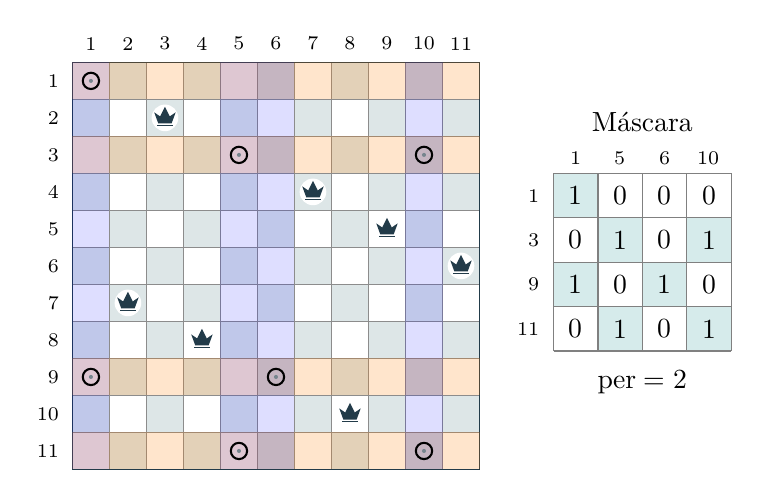
\begin{tikzpicture}[x=.47cm,y=.47cm]
 \bcuadricula{11}
 \foreach \rr in {1,3,9,11}{\fill[orange,opacity=.20] (0,{11-\rr}) rectangle (11,{12-\rr});}
 \foreach \cc in {1,5,6,10}{\fill[blue,opacity=.13] ({\cc-1},0) rectangle (\cc,11);}
 \foreach \rr/\cc in {1/1,3/5,3/10,9/1,9/6,11/5,11/10}{
  \bmarca{11}{\rr}{\cc}
  \draw[black,line width=.75pt] ({\cc-.5},{11.5-\rr}) circle[radius=.22];
 }
 \foreach \rr/\cc in {2/3,4/7,5/9,6/11,7/2,8/4,10/8}{\breina{11}{\rr}{\cc}}
 \begin{scope}[shift={(13,3.2)},scale=1.2]
  \node at (2,5.15) {Máscara};
  \foreach \indice/\original in {1/1,2/5,3/6,4/10}
   {\node[font=\scriptsize] at ({\indice-.5},4.35) {$\original$};}
  \foreach \indice/\original in {1/1,2/3,3/9,4/11}
   {\node[font=\scriptsize,anchor=east] at (-.1,{4.5-\indice}) {$\original$};}
  \foreach \rr/\cc in {1/1,2/2,2/4,3/1,3/3,4/2,4/4}
   {\fill[teal!16] ({\cc-1},{4-\rr}) rectangle (\cc,{5-\rr});}
  \draw[step=1,gray,line width=.45pt] (0,0) grid (4,4);
  \foreach \rr/\valores in {1/{1,0,0,0},2/{0,1,0,1},3/{1,0,1,0},4/{0,1,0,1}}{
   \foreach \valor [count=\cc] in \valores
    {\node at ({\cc-.5},{4.5-\rr}) {$\valor$};}
  }
  \node at (2,-.7) {$\operatorname{per}=2$};
 \end{scope}
\end{tikzpicture}
\caption{Tablero de orden once de la solución $\pi=(1,3,5,7,9,11,2,4,6,8,10)$ después de retirar las
reinas de las filas $1,3,9,11$. Las filas se numeran desde uno de arriba abajo y las columnas desde
uno de izquierda a derecha. Quedan siete reinas, dibujadas con coronas. Las bandas destacan las cuatro
filas vacías y las columnas vacías $1,5,6,10$. Los puntos rodeados señalan las casillas disponibles y
corresponden a los unos de la máscara, que conserva las etiquetas originales. La fila $1$ fuerza la
columna $1$ y entonces la fila $9$ fuerza la $6$. Las filas $3$ y $11$ pueden intercambiar $5$ y $10$,
de donde resulta el permanente $2$. Las diferencias positivas entre filas son $2,6,8,10$ y entre
columnas son $1,4,5,9$. Como los dos conjuntos son disjuntos, los cruces vacíos no comparten
diagonal.}\label{fig:terminal}
\end{figure}


Recordamos que $F$ es el suceso de permanencia de la Definición~\ref{def:regular}: la historia llega
al tamaño $K$ y todos sus tableros, incluido el de llegada $B^{(K)}$, son regulares. La figura ilustra la
geometría. En ella la fila 1 fuerza la
columna 1, por lo que toda matriz bistocástica sobre la máscara asigna masa cero a la casilla
disponible $(9,1)$. El ejemplo queda fuera de $F$. Sea
$D_K$ el suceso de que dos cruces vacíos distintos del tablero de tamaño $K$ pertenezcan a una misma
diagonal del tablero inicial. Para $m\ge 1$ escribimos
$(u)_m=u(u-1)\cdots(u-m+1)$ si
$u\ge m$, y $(u)_m=0$ si $0\le u<m$.

\begin{lema}[Diagonales compartidas en el último tablero]\label{terminal-geometria}
Bajo $\nu$ y bajo la ley $\mu$ de una solución uniforme revelada en orden uniforme independiente,
respectivamente,
\[
 \nu(F\cap D_K)\le d_{n,K}:=\frac{C K^4}{n}\,e^{C'/K},
 \qquad \mu(D_K\mid\pi)\le \frac{C K^4}{n}
\]
para toda solución $\pi$. La segunda probabilidad es respecto del orden de
revelado.
\end{lema}
\begin{proof}
En el tablero inicial hay a lo sumo $Cn^3$ pares de casillas distintas que comparten diagonal. Se
elige la primera entre $n^2$ casillas y la segunda entre a lo sumo $2(n-1)$ casillas de sus
diagonales. Para que las dos casillas de un par sean cruces vacíos en el tamaño $K$ deben quedar
vacías dos filas distintas y dos columnas distintas. En $F$ no hubo salida anterior, de modo que
\eqref{prescr} con
$s=t=2$ acota la probabilidad de cada par por $(K/n)^4e^{C'/K}$. La unión da la primera afirmación.

Para la segunda afirmación fijemos $\pi$. Las últimas $K$ filas en el orden uniforme forman un
subconjunto uniforme $I$ de tamaño $K$. Las columnas correspondientes son $\pi(I)$ y los cruces vacíos
forman $I\times\pi(I)$. La Figura~\ref{fig:testigos} muestra cómo intervienen las etiquetas de fila en
dos de esos cruces.
\begin{figure}[htbp]
\centering
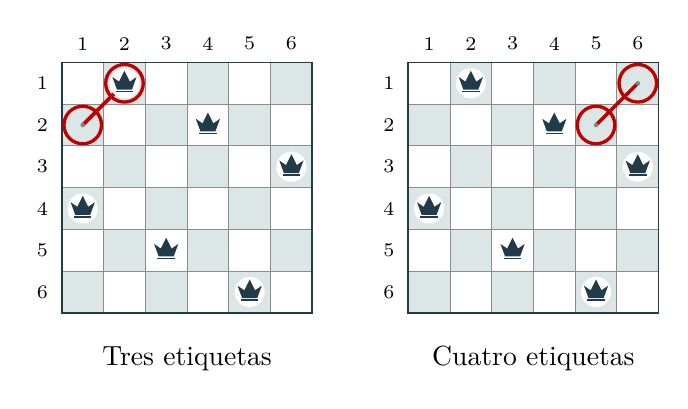
\begin{tikzpicture}[x=.53cm,y=.53cm]
 \foreach \tipo/\dx/\uno/\dos in {3/0/2/1,4/8.3/6/5}{
  \begin{scope}[shift={(\dx,0)}]
   \bcuadricula{6}
   \draw[red!75!black,line width=1.3pt] ({\uno-.5},5.5) -- ({\dos-.5},4.5);
   \bmarca{6}{1}{\uno}
   \bmarca{6}{2}{\dos}
   \draw[red!75!black,line width=1.2pt] ({\uno-.5},5.5) circle[radius=.45];
   \draw[red!75!black,line width=1.2pt] ({\dos-.5},4.5) circle[radius=.45];
   \foreach \rr/\cc in {1/2,2/4,3/6,4/1,5/3,6/5}{\breina{6}{\rr}{\cc}}
   \ifnum\tipo=3
    \node at (3,-1.1) {Tres etiquetas};
   \else
    \node at (3,-1.1) {Cuatro etiquetas};
   \fi
  \end{scope}
 }
\end{tikzpicture}
\caption{Dos testigos en el tablero de orden seis de la solución $\pi=(2,4,6,1,3,5)$. Las filas se
numeran desde uno de arriba abajo y las columnas desde uno de izquierda a derecha. Las coronas son las
reinas de $\pi$. Dos círculos unidos señalan las casillas $(i,\pi(j))$ e $(i',\pi(j'))$ que comparten
diagonal. A la izquierda, $(i,i',j,j')=(1,2,1,4)$ marca $(1,2)$ y $(2,1)$ y usa tres etiquetas
distintas. A la derecha, $(1,2,3,6)$ marca $(1,6)$ y $(2,5)$ y usa cuatro. Con sólo dos etiquetas se
tendría $\{i,i'\}=\{j,j'\}$ y $|i-i'|=|\pi(i)-\pi(i')|>0$, lo que haría que dos reinas de la solución
se atacasen.}\label{fig:testigos}
\end{figure}


Un par que comparte diagonal se escribe $(i,\pi(j)),(i',\pi(j'))$, con
\[
 |i-i'|=|\pi(j)-\pi(j')|>0,\qquad i,i',j,j'\in I.
\]
Llamamos \emph{testigo} a una cuádrupla de etiquetas $(i,i',j,j')$ que cumple esta igualdad de
distancias, pertenezcan o no a $I$. Pongamos $m=|\{i,i',j,j'\}|$. Si $m=2$, los pares de etiquetas
$\{i,i'\}$ y $\{j,j'\}$ coinciden. La
igualdad de distancias diría que las reinas de $\pi$ en las filas $i,i'$ se atacan, lo que es imposible.
Si $m=3$, fijamos $i,i'$ y cuál de las dos etiquetas se repite en cuál de las posiciones $j,j'$. La
imagen bajo $\pi$ de esa etiqueta es conocida. La otra imagen debe estar a distancia $|i-i'|$ de ella,
por lo que tiene a lo sumo dos valores posibles. Cada uno determina su etiqueta mediante $\pi^{-1}$.
Hay por tanto $O(n^2)$ testigos con tres etiquetas. Para $m=4$, fijar $i,i',j$ deja a lo sumo dos
valores para $\pi(j')$, y da $O(n^3)$ testigos.

El subconjunto $I$ contiene $m$ etiquetas fijadas con probabilidad $(K)_m/(n)_m\le(K/n)^m$ cuando
$n\ge m$. Para $n\ge4$ resulta por unión
\[
 \mu(D_K\mid\pi)\le C\left[n^2(K/n)^3+n^3(K/n)^4\right]\le CK^4/n.
\]
Bajo $\mu$, la solución y el orden se pueden completar también para historias ya detenidas. Como
$F\cap D_K\subseteq D_K$, integrar la estimación respecto de $\pi$ da también $\mu(F\cap D_K)\le
CK^4/n$.
\end{proof}

\begin{lema}[Reducción a torres en el último tablero]\label{terminal-pivotes}
Sea $A$ la máscara del tablero $B^{(K)}$. En $F\cap D_K^c$ hay una
colocación que completa el tablero y
\[
 Q(B^{(K)})=\per A,\qquad L(B^{(K)})=L_T(A),
\]
donde $L_T(A)=H_T(p)+\log\Gamma_2$ es el predictor de torres en el mismo soporte, como en el modelo
de torres con máscara de~\cite[Secciones~8.1 y~8.5]{pred}. Aquí $H_T(p)=-\sum_e p_e\log p_e
+\sum_e(1-p_e)\log(1-p_e)$ es la entropía de torres, evaluada en su punto estacionario con masas
de fila y de columna iguales a uno, y $\Gamma_2$ es el factor de la
Sección~\ref{costes:permanente}.
\end{lema}
\begin{proof}
En $F$ el punto de Bethe $p$ de $B^{(K)}$ tiene masas de fila y de columna iguales a uno y es positivo en
todas las casillas disponibles. Para un conjunto cualquiera $I$ de filas, toda su masa $|I|$ llega al
conjunto
de columnas vecinas, que admite a lo sumo una unidad por columna. En consecuencia $|\mathcal
N(I)|\ge|I|$. Para ver directamente que se puede cubrir toda fila, tómese un emparejamiento de
cardinal máximo. Si deja una fila sin cubrir, desde todas las filas descubiertas se recorren
alternativamente aristas fuera del emparejamiento desde las filas y aristas del emparejamiento desde
las columnas. Una columna descubierta alcanzable daría un camino aumentante, contradicción. Luego cada
columna alcanzable está emparejada con una fila alcanzable, y estas filas emparejadas no agotan las
filas alcanzables, entre las que hay una descubierta. Todas las vecinas de una fila alcanzable son
alcanzables, incluida, si existe, la columna por la que se entró en esa fila. Esto contradice la
desigualdad para el conjunto de filas alcanzables. Así $\per A>0$.

En $D_K^c$, cada diagonal contiene a lo sumo un cruce vacío. Toda permutación del
soporte respeta por ello las dos restricciones diagonales. Además, las casillas de diagonales ocupadas
ya se excluyeron al formar $A$, por lo que cualquier permutación del soporte da una completación legal
de $B^{(K)}$. La construcción es reversible y prueba $Q(B^{(K)})=\per A$.

En una diagonal libre con una casilla disponible $e$, la vacancia es $h_f=1-p_e=:q_e$. Cada casilla
tiene dos de estas diagonales y una diagonal libre sin casillas tiene $h_f=1$. Así en $H_B$ los
términos diagonales restan dos copias de $\sum_e q_e\log q_e$, y queda exactamente la entropía de
torres
\[
 H_T(p)=-\sum_e p_e\log p_e+\sum_e q_e\log q_e .
\]
La ecuación estacionaria del Lema~\ref{coste-vacancias} pasa a ser $p_eq_e=a_ib_j$ en toda casilla
disponible, con los mismos $a_i,b_j$. También se obtiene $H_B=H_T$
directamente como identidad de los funcionales en los puntos factibles del soporte: en toda diagonal
de una sola casilla la vacancia siempre es el complemento de la única entrada. De aquí que el punto
de Bethe sea también el punto estacionario del predictor de torres.

Queda verificar el normalizador, como en \cite[Sección~8.1]{pred}. Para una casilla de masa $p$
ponemos $q=1-p$, $\tau_d=pq/(1-dp)$ y $b_d=(1-dp)/q^d$. Al eliminar la coordenada de su primera
diagonal, el pivote en $S_4$ es $q+\tau_4$. Si $r$ indica las otras líneas de la casilla, la
contribución $\tau_4rr^T$ en el bloque restante se sustituye, por el complemento de Schur, por
$(\tau_4-\tau_4^2/(q+\tau_4))rr^T$. La segunda diagonal de esa casilla se elimina después con $d=3$.
En ambos pasos
\[
 q+\tau_d=\frac{q(1-(d-1)p)}{1-dp},\qquad
 \tau_d-\frac{\tau_d^2}{q+\tau_d}=\tau_{d-1},\qquad
 b_d(q+\tau_d)=b_{d-1}.
\]
Dado que la diagonal eliminada tiene una sola casilla, la operación afecta sólo a la contribución de
esa casilla. Una línea sin casillas tiene pivote uno y no afecta a las otras coordenadas. El modo cero
$(\mathbf1_R,-\mathbf1_C,0)$ tiene coordenada cero en cada línea eliminada. Por ello podemos calcular
el pseudodeterminante en una base ortonormal de su complemento que contenga los vectores de las
diagonales eliminadas. Allí la factorización ordinaria por los pivotes es exacta y el modo de filas y
columnas conserva su longitud $\sqrt{2K}$. El factor correspondiente del normalizador es
$\sqrt{2\pi}\sqrt{2K}=\sqrt{4\pi K}$ tanto antes como después. Como $e^{C_d}=\prod_e b_d(p_e)$, las
identidades prueban
$e^{C_4}\pdet S_4=e^{C_2}\pdet S_2$ tras completar las dos eliminaciones por casilla. En particular
$\Gamma_4=\Gamma_2$. Esto da $L(B^{(K)})=H_T(p)+\log\Gamma_2=L_T(A)$.
\end{proof}

\subsection{Difusión, escalado y determinante}\label{permanente}

En esta subsección $K$ es el orden de una matriz bistocástica $P$ y $J_K=\mathbf1\mathbf1^T/K$. Las
estimaciones valen asimismo con $K=k$ al aplicarlas en la Sección~\ref{costes}. Las cotas
exteriores fijan constantes $M_0$ y $\rho_*<1$ tales que
\begin{equation}\label{terminal-hipotesis-matriz}
 0\le P_{ij}\le M_0/K,\qquad \|P-J_K\|_{\rm op}\le\rho_* .
\end{equation}
En efecto, para una matriz bistocástica, el bloque de filas y columnas con pesos $P$ es
$\left(\begin{smallmatrix}I&P\\P^T&I\end{smallmatrix}\right)$; sus autovalores son $1\pm\sigma_j(P)$.
Las dos rectas constantes corresponden al valor singular uno. Una brecha $\gamma>0$ fuera del modo
cero implica que los restantes valores singulares son a lo sumo $1-\gamma$, que es precisamente la
cota requerida para $P-J_K$.

\begin{lema}[Escalado bistocástico]\label{terminal-escalado}
Supongamos \eqref{terminal-hipotesis-matriz} y escribamos
$W_{ij}=P_{ij}(1-P_{ij})$ y $a_K=\sum_{ij}P_{ij}^2$. Para $K$ suficientemente grande hay vectores
$\alpha,\beta$ con $\sum_i\alpha_i=\sum_j\beta_j$ tales que $D_{ij}=e^{\alpha_i+\beta_j}W_{ij}$ es
bistocástica. Además,
\[
 \max\{\|\alpha\|_\infty,\|\beta\|_\infty\}=O(K^{-1}),\qquad
 \sum_i\alpha_i+\sum_j\beta_j=a_K+O(K^{-1}),\qquad
 \|D-P\|_{\rm HS}=O(K^{-1}).
\]
Las constantes dependen sólo de $M_0,\rho_*$. El soporte de $D$ coincide con el de $P$.
\end{lema}
\begin{proof}
Para controlar la precisión del escalado, tratado en general en \cite{sk}, consideremos $S=PP^T$. Es
simétrica y bistocástica, con $S_{ij}\le M_0/K$ y $\|S-J_K\|_{\rm op}\le\rho_*^2$, pues
$S-J_K=(P-J_K)(P-J_K)^T$. Cada fila de $S-J_K$ tiene norma euclídea al cuadrado
$\sum_j S_{ij}^2-1/K\le (M_0-1)/K$. Como $S^t-J_K=(S-J_K)^t$ para todo entero $t\ge1$, multiplicar una
fila de $S-J_K$ por $(S-J_K)^{t-1}$ y pasar de norma euclídea a norma de suma absoluta da
\[
 \|S^t-J_K\|_{\infty\to\infty}
 \le \sqrt{M_0-1}\,\rho_*^{\,2(t-1)} .
\]
En los vectores de media cero, la serie $\sum_{t\ge0}S^t$ es por tanto la inversa de $I-S$ y tiene
norma $\infty\to\infty$ uniformemente acotada. La misma prueba con $P^TP$ da la cota para
$(I-P^TP)^{-1}$ en ese subespacio.

Pongamos $S_0=\left(\begin{smallmatrix}I&P\\P^T&I\end{smallmatrix}\right)$.
En el subespacio $\sum x=\sum y$, la ecuación $S_0(x,y)=(f,g)$ se plantea para $\sum f=\sum g$. Si
$s=K^{-1}\sum f$, la eliminación en los dos bloques da
\[
 \begin{aligned}
 x&=\tfrac12s\mathbf1+(I-PP^T)^{-1}(f-Pg),\\
 y&=\tfrac12s\mathbf1+(I-P^TP)^{-1}(g-P^Tf).
 \end{aligned}
\]
Los argumentos de ambas inversas tienen media cero. La parte constante viene de que $x+Py=f$ y
$y+P^Tx=g$ tienen ambas media $s$ y las medias de $x,y$ coinciden. Como
$\|P\|_{\infty\to\infty}=\|P^T\|_{\infty\to\infty}=1$, la inversa $T$ de $S_0$ con este gauge
satisface $\|T\|_{\infty\to\infty}\le C_1(M_0,\rho_*)$.

Sea $\Psi(\alpha,\beta)$ el vector formado por las sumas de filas y de columnas de
$(e^{\alpha_i+\beta_j}W_{ij})$ menos
uno por coordenada. Sus dos sumas son iguales. En cero el defecto es a lo sumo $M_0/K$ por
$\sum_jP_{ij}^2\le M_0/K$ y su análoga en columnas. En una bola de radio $r\le1$ la derivada de $\Psi$
tiene en los bloques diagonales las sumas de filas y de columnas de la matriz escalada en el punto
considerado, y esa matriz y su traspuesta en los bloques cruzados. En cada fila y columna
\[
 \sum_j\big|e^{\alpha_i+\beta_j}W_{ij}-P_{ij}\big|
 \le C_2(r+K^{-1})\sum_jP_{ij}=C_2(r+K^{-1}),
\]
con la misma desigualdad al sumar en $i$. Se usaron $|\alpha_i+\beta_j|\le2r$ y $P_{ij}\le M_0/K$. Así
$\|\Psi'-S_0\|_{\infty\to\infty}\le 2C_2(r+K^{-1})$.

En el gauge fijado, el mapa $u\mapsto u-T\Psi(u)$ desplaza el origen a distancia a lo sumo
$C_1M_0/K$. Tomemos la bola cerrada de radio $r=2C_1M_0/K$. Para $K$ grande su derivada tiene norma a
lo sumo $2C_1C_2(r+K^{-1})\le1/2$. Conserva por tanto la bola y es una contracción. Su punto fijo
resuelve $\Psi=0$ y tiene norma $O(K^{-1})$. Como $P_{ij}<1$ para $K$ grande, el factor
$(1-P_{ij})e^{\alpha_i+\beta_j}$ es positivo y conserva el soporte.

Uniformemente en los índices tenemos ahora
\[
 D_{ij}=P_{ij}\bigl(1+\alpha_i+\beta_j-P_{ij}+O(K^{-2})\bigr).
\]
Sumamos en $i,j$. Puesto que tanto $D$ como $P$ tienen masa total $K$, y las sumas de filas y de
columnas de $P$ valen uno,
obtenemos $\sum_i\alpha_i+\sum_j\beta_j-a_K=O(K^{-1})$. Por otra parte, $|D_{ij}-P_{ij}|\le
C_3P_{ij}/K$ y $a_K\le M_0$. Elevar al cuadrado y sumar prueba la afirmación en norma de
Hilbert--Schmidt.
\end{proof}

\begin{proposicion}[Permanente de la matriz auxiliar]\label{terminal-permanente}
Para las matrices del Lema~\ref{terminal-escalado}, pongamos $B=P-J_K$. Uniformemente bajo
\eqref{terminal-hipotesis-matriz} se cumple
\[
 \log\frac{\per W}{\prod_{ij}(1-P_{ij})}
 =\tfrac12\log(2\pi K)-\tfrac12a_K
   -\tfrac12\log\det(I-B^TB)+o(1).
\]
\end{proposicion}
\begin{proof}
Usamos la estimación de McCullagh~\cite{mccullagh} en la forma de \cite[Proposición~3.1]{dw}. Si
$D=J_K+B_D$ es bistocástica, $\max_{ij}|B_{D,ij}|\le A_0/K$ y $\|B_D\|_{\rm op}\le\rho_0<1$, entonces
\[
 \frac{K^K\per D}{K!}=(1+o(1))\det(I-B_D^TB_D)^{-1/2}.
\]
En \cite[Sección~2.1]{dw} una matriz bistocástica es no negativa, con filas y columnas de suma uno,
de modo que se admiten entradas nulas. Divoux y Wang demuestran la estimación con un error relativo
que tiende a cero uniformemente en la clase de matrices con cotas $A_0,\rho_0$ fijas
\cite[Observación~2.1]{dw}, que es la forma que necesitamos. La uniformidad también se deduce del
enunciado para sucesiones, con una matriz en cada orden. Si fallase, habría un $\epsilon>0$ y órdenes
crecientes $K_j$ con matrices
en esta clase y error relativo al menos $\epsilon$. Al completar esos órdenes con la matriz $J_K$ en
cada orden restante $K$ se obtendría una sucesión con las mismas dos cotas para la que fallaría la
proposición citada.

Sea $D$ el escalado del Lema~\ref{terminal-escalado}. Puesto que $D_{ij}=P_{ij}(1+O(K^{-1}))$, sus
entradas están acotadas por $C/K$ y $\max|B_{D,ij}|\le A_0/K$. Si fijamos $\rho_*<\rho_0<1$, entonces
\[
 \|B_D\|_{\rm op}\le\|P-J_K\|_{\rm op}+\|D-P\|_{\rm HS}
       \le\rho_0
\]
para $K$ suficientemente grande, uniformemente. Por otra parte,
$\|B\|_{\rm HS}^2=a_K-1=O(1)$ y $\|B_D\|_{\rm HS}=O(1)$. Usando
$\|X^TY\|_1\le\|X\|_{\rm HS}\|Y\|_{\rm HS}$ para la norma traza, obtenemos
\[
 \|B_D^TB_D-B^TB\|_1
 \le(\|B_D\|_{\rm HS}+\|B\|_{\rm HS})\|D-P\|_{\rm HS}
 =O(K^{-1}).
\]
Para todo punto $H$ del segmento entre ambos productos de Gram se cumple $0\le H\le\rho_0^2I$. La
derivada de $\log\det(I-H)$ en dirección $U$ es $-\operatorname{tr}((I-H)^{-1}U)$, de módulo a lo sumo
$\|U\|_1/(1-\rho_0^2)$. Integrar sobre el segmento permite sustituir $B_D$ por $B$ dentro del
logaritmo del determinante, con error $O(K^{-1})$.

Cada producto de una permutación recibe en el escalado el mismo factor $\exp(\sum\alpha+\sum\beta)$.
Luego
\[
 \log\per W=\log\per D-a_K+O(K^{-1}).
\]
Finalmente, $\sum_{ij}P_{ij}=K$, $\sum_{ij}P_{ij}^3=O(K^{-1})$ y Taylor da
$-\sum_{ij}\log(1-P_{ij})=K+a_K/2+O(K^{-1})$. Aplicando a $D$ la estimación citada y usando
$\log(K!/K^K)=-K+\tfrac12\log(2\pi K)+O(K^{-1})$, obtenemos la fórmula anunciada. Todas las
perturbaciones y la elección de $A_0,\rho_0$ son uniformes para los parámetros de
\eqref{terminal-hipotesis-matriz}.
\end{proof}

\begin{lema}[Identificación con el factor de torres]\label{terminal-normalizador}
Con los pesos del Lema~\ref{terminal-escalado},
\[
 \log\frac{\per W}{\prod_{ij}(1-P_{ij})}=\log\Gamma_2+o(1)
\]
uniformemente bajo \eqref{terminal-hipotesis-matriz}.
\end{lema}
\begin{proof}
Para $S_0=\left(\begin{smallmatrix}I&P\\P^T&I\end{smallmatrix}\right)$ el autovalor constante positivo
es dos, el otro constante es nulo y, fuera de esas rectas, los valores singulares de $P-J_K$ producen
los factores $(1-\sigma)(1+\sigma)$. Por tanto
\[
 \pdet S_0=2\det(I-B^TB).
\]
El bloque de incidencia de torres es $S_2=S_0+\Delta$, donde, con $\iota_e$ el vector indicador de la
fila y la
columna de la casilla $e$,
\[
 \Delta=\sum_e\bigl(\tau_2(P_e)-P_e\bigr)\iota_e\iota_e^T,\qquad
 \tau_2(P_e)-P_e=\frac{P_e^2}{1-2P_e}.
\]
La matriz $\Delta$ es positiva semidefinida y anula el modo cero. Las sumas absolutas en una fila de
$\Delta$ son $O(K^{-1})$ porque $P$ es bistocástica y $P_{ij}\le M_0/K$, luego $\|\Delta\|_{\rm
op}=O(K^{-1})$. Además
$\operatorname{tr}\Delta=2\sum_e P_e^2/(1-2P_e)=2a_K+O(K^{-1})$ y
$\|\Delta\|_{\rm HS}^2\le\|\Delta\|_{\rm op}\operatorname{tr}\Delta=O(K^{-1})$.

El complemento del modo cero de $S_0$ tiene brecha al menos $1-\rho_*$. Allí ponemos
$X=S_0^{-1/2}\Delta S_0^{-1/2}$. Se tiene $X\ge0$ y $\|X\|_{\rm HS}^2=O(K^{-1})$. Aplicando
$|\log(1+x)-x|\le x^2/2$ para $x\ge0$ obtenemos
\[
 \log\pdet S_2-\log\pdet S_0
 =\operatorname{tr}(S_0^+\Delta)+O(K^{-1}).
\]
Para estimar la traza observemos que $\|S_0^+-I\|_{\rm HS}=O(1)$. En las rectas constantes esto es
inmediato. En el complemento de ambas, $S_0-I$ tiene bloques cruzados $B,B^T$ y por tanto norma de
Hilbert--Schmidt $O(1)$. Multiplicarlo por la inversa acotada $-S_0^{-1}$ da allí $S_0^{-1}-I$. La
desigualdad de Cauchy--Schwarz para la traza muestra entonces que
\[
 |\operatorname{tr}((S_0^+-I)\Delta)|\le
 \|S_0^+-I\|_{\rm HS}\|\Delta\|_{\rm HS}=O(K^{-1/2}).
\]
En conclusión,
\[
 \log\pdet S_2=\log 2+\log\det(I-B^TB)+2a_K+O(K^{-1/2}).
\]
El término local es
$C_2=\sum_{ij}(\log(1-2P_{ij})-2\log(1-P_{ij}))=-a_K+O(K^{-1})$.
Al sustituir ambos desarrollos en
$\log\Gamma_2=(\log(4\pi K)-C_2-\log\pdet S_2)/2$
se recupera el lado derecho de la Proposición~\ref{terminal-permanente}, con diferencia $o(1)$
uniforme.
\end{proof}

\begin{proposicion}[Error en el último tablero]\label{terminal-error}
Existe una sucesión $\theta_K\to0$, dependiente sólo de las cotas exteriores, tal que en
$F\cap D_K^c$
\[
 |\log Q(B^{(K)})-L(B^{(K)})|\le\theta_K .
\]
Si $G=F\cap\{Q(B^{(K)})>0\}$, entonces $\nu(G)\ge\nu(F)-d_{n,K}$. Para $L_K^{\max}=C K\log(K+1)$ y
$\nu(G)>0$ se cumplen
\[
 \begin{aligned}
 \E_\mu\!\left[|g(B^{(K)})|\mathbf1_F\right]
 &\le\theta_K+(L_K^{\max}+\log K!)\, CK^4/n,\\
 \E_{\nu(\cdot\mid G)}[g(B^{(K)})^-]
 &\le\theta_K+L_K^{\max}\,d_{n,K}/\nu(G).
 \end{aligned}
\]
Aquí $u^-=\max\{-u,0\}$.
\end{proposicion}
\begin{proof}
En $F\cap D_K^c$ tomemos $P=(p_{ij})$ igual al punto de Bethe, extendido por cero fuera de $A$. El
Lema~\ref{terminal-pivotes} da $H_B=H_T$, $L=H_T+\log\Gamma_2$ y $Q(B^{(K)})=\per A>0$. La estacionariedad
de torres dice que $W_{ij}=a_i b_j$ en todo el soporte de $A$. Sea
$\mathcal K_T=\prod_i a_i\prod_j b_j$.
Al multiplicar los pesos de una permutación y sumar obtenemos $\per W=\mathcal K_T\,\per A$. Al
ponderar con $P_{ij}$ los logaritmos de $P_{ij}(1-P_{ij})=a_i b_j$ sobre las casillas disponibles y
usar que las masas de fila y de columna valen uno, se obtiene
\[
 H_T(P)=-\log\mathcal K_T+\sum_{ij}\log(1-P_{ij}).
\]
Por consiguiente
\[
 \log\per A-H_T(P)
 =\log\frac{\per W}{\prod_{ij}(1-P_{ij})}.
\]
El Lema~\ref{terminal-normalizador} da la primera conclusión por su uniformidad sobre los posibles
tableros en $F$. En particular $F\cap D_K^c\subseteq G$, de donde $\nu(G)\ge\nu(F)-d_{n,K}$ por el
Lema~\ref{terminal-geometria}.

En el resto de $F$ usamos directamente la entropía del predictor completo. En cada fila, $-\sum_j
p_{ij}\log p_{ij}\le\log K$, mientras que $0\le -(1-y)\log(1-y)\le y$ para $0\le y\le1$. Sumando sobre
casillas y sobre diagonales, con $\sum_e p_e=K$ y $\sum_f\ell_f=2K$, se deduce
\[
 -3K\le H_B(p)\le K\log K+2K .
\]
El Lema~\ref{coste-estatico} da entonces $|L(B^{(K)})|\le L_K^{\max}$ para $K$ suficientemente grande.
En una historia que se puede completar, $1\le Q(B^{(K)})\le K!$, de modo que
$|g(B^{(K)})|\le L_K^{\max}+\log K!$ y $g(B^{(K)})^-\le L_K^{\max}$.

Bajo $\mu$ las historias siempre se pueden completar. Aplicamos la primera conclusión en $F\cap D_K^c$
y la última cota absoluta en $F\cap D_K$, cuya probabilidad es a lo sumo $CK^4/n$ al promediar el
Lema~\ref{terminal-geometria} sobre $\pi$. Bajo $\nu(\cdot\mid G)$ la historia también es completable,
y la probabilidad de $D_K$ es a lo sumo $\nu(F\cap D_K)/\nu(G)\le d_{n,K}/\nu(G)$. La primera
conclusión en $D_K^c$ y la cota de $g^-$ en $D_K$ dan la segunda desigualdad.
\end{proof}

\section{Comparación final de los conteos}\label{balance}
\begin{proof}[Demostración del Teorema~\ref{princ}]
Fijamos las constantes de las clases, $a_{\rm mes}$, $\varrho_{\rm mes}$ y las tolerancias,
$\varepsilon$, $\delta$, $K_0$, $\varrho_{\rm mac}$ y $a_{\rm mac}$ en el orden de la
Sección~\ref{meso:constantes}. Sea $K\ge K_0$ un entero fijo. Distinguimos la primera salida
macroscópica $E_{\rm mac}$, la primera salida en la banda de tamaño $2^jK$ denotada por $E_j$
y la permanencia $F$. Atribuimos cada salida a la banda del padre que conduce a ella,
incluyendo el hijo alcanzado. Las bandas se pueden desplazar un paso en la estimación de la
Proposición~\ref{prop:salida-banda-meso}, cambiando la constante multiplicativa. Un fallo de
entrada en el corte $k=M$ pertenece a $E_{\rm mac}$. Los sucesos forman una partición.

Sea $\Lambda$ la función de la historia detenida que vale $\Lambda_{\rm mac}=C_\delta n^{2/3}$ en
$E_{\rm mac}$, $\Lambda_j=C_0+2\beta(\varepsilon_{\rm out})2^jK$ en $E_j$, y cero en $F$.
La Proposición~\ref{coste-macro} y el Corolario~\ref{coste-debil} se aplican al tablero de primera
salida, porque su padre regular garantiza las cotas exteriores en él. Se tiene
$g(B_\tau)\mathbf1_{F^c}\le\Lambda$ en las historias con masa positiva bajo $\mu$.

Aplicamos la desigualdad variacional de Gibbs~\cite[cap.~2]{ct} a $\Lambda$ y a las leyes de
las historias detenidas. En este espacio finito se obtiene directamente por Jensen,
restringiendo la suma bajo $\nu$ al soporte de $\mu$:
\[
 \E_\mu\Lambda-D(\mu^\tau\Vert\nu^\tau)\le\log\E_\nu e^\Lambda
 =\log\!\left(1+\nu(E_{\rm mac})(e^{\Lambda_{\rm mac}}-1)
              +\sum_{j\ge0}\nu(E_j)(e^{\Lambda_j}-1)\right).
\]
El Corolario~\ref{macro:cambio} y la estimación de entrada en la Sección~\ref{meso}
acotan el sumando macroscópico por $C_1\exp(-c_1n+C_\delta n^{2/3})$, con $C_1,c_1>0$ que dependen
de $\delta$ y de $\varrho_{\rm mac}$.
Para las bandas, la Proposición~\ref{prop:salida-banda-meso} da una tasa
$c>2\beta(\varepsilon_{\rm out})$. Tomando $c'$ menor que la diferencia, la suma de
$\exp[-(c-2\beta(\varepsilon_{\rm out}))2^jK]$ es $O(e^{-c'K})$ para $K$ grande.
El Corolario~\ref{hist:consistencia}, \eqref{super} y la estimación terminal bajo $\mu$
de la Proposición~\ref{terminal-error} dan
\[
 \limsup_{n\to\infty}g(B_0)\le C/K+\theta_K+Ce^{-c'K},\qquad\theta_K\to0 .
\]
En efecto, a $K$ fijo el coste excepcional terminal es a lo sumo
$C_K K^4/n$, que tiende a cero antes de tomar el límite en $K$.

Para la otra desigualdad usamos $G=F\cap\{Q(B_K)>0\}$. Por la estimación geométrica bajo
$\nu$ de la Sección~\ref{terminal}, $s=\nu(G)\ge1-Ce^{-cK}-o_n(1)-d_{n,K}$, donde
$d_{n,K}\to0$ a $K$ fijo. Para $K$ grande este límite inferior es positivo. La parte
negativa del coste terminal excepcional tiene esperanza bajo $\nu(\cdot\mid G)$ a lo sumo
$C_Kd_{n,K}/s$. En las historias restantes basta $\theta_K$. Tomando el límite inferior en
\eqref{infer} y usando $\log(1-z)\ge-2z$ para $0\le z\le1/2$ obtenemos
\[
 \liminf_{n\to\infty}g(B_0)\ge-C/K-\theta_K-Ce^{-cK}.
\]
Hacemos tender ahora $K$ a infinito en las dos desigualdades. En el tablero inicial $B_0$, el
máximo global de la Proposición~\ref{macro:maximo} satisface $p_{\max}<1/4$ para $n$ grande y,
por tanto, coincide con el maximizador canónico de~\cite{pred}. La relación entre el cofactor y el
pseudodeterminante de la Sección~\ref{leyes} da $L(B_0)=\log Q_{\rm pred}(n)$. Resulta
$g(B_0)=\log Q(n)-\log Q_{\rm pred}(n)\to0$. Aplicar el Teorema~1.1 de~\cite{pred} al
segundo logaritmo identifica la constante que aparece en el enunciado.
\end{proof}

\section{Discusión}
La reducción a un permanente ocurre después de elegir las últimas filas. El orden uniforme
permite probar la cota geométrica incluso para una solución fija. Bajo la ley adaptativa,
el mismo fenómeno se obtiene a partir de las probabilidades de que sobrevivan filas y columnas
prescritas. Esta distinción explica por qué las dos cotas para el conteo admiten un mismo
último tablero aunque sus historias tengan distribuciones diferentes.

La estimación del permanente es uniforme en una clase con cotas de difusión y de brecha fijas. Su resto
tiende a cero al crecer el tamaño del último tablero. El orden de límites de la
Sección~\ref{balance} permite utilizar precisamente esa información. Para obtener la tasa
$O(1/n)$ de la Conjetura~10.1 de~\cite{pred} sería necesario controlar cuantitativamente
el error terminal y su dependencia del suelo $K$.

\section*{Uso de herramientas de inteligencia artificial}
\addcontentsline{toc}{section}{Uso de herramientas de inteligencia artificial}

Se utilizaron herramientas de inteligencia artificial para organizar las fuentes, cotejar
versiones, preparar la composición y la reestructuración editorial del texto, y realizar revisiones
adversariales de extractos textuales.

\begin{thebibliography}{99}
\raggedright

\bibitem{bk} C.~Bowtell y P.~Keevash, \emph{The $n$-queens problem}, arXiv:2109.08083v1 (2021).
\href{https://doi.org/10.48550/arXiv.2109.08083}{doi:10.48550/arXiv.2109.08083}.

\bibitem{ct} T.~M.~Cover y J.~A.~Thomas, \emph{Elements of Information Theory}, 2.ª ed., Wiley,
2006. \href{https://doi.org/10.1002/047174882X}{doi:10.1002/047174882X}.

\bibitem{dw} A.~Divoux y S.~Wang, \emph{The maximum number of Hamiltonian cycles in tournaments},
arXiv:2610.23755v1 (2026).
\href{https://doi.org/10.48550/arXiv.2610.23755}{doi:10.48550/arXiv.2610.23755}.

\bibitem{ls} Z.~Luria y M.~Simkin, \emph{A lower bound for the $n$-queens problem}, en
\emph{Proceedings of the 2022 Annual ACM-SIAM Symposium on Discrete Algorithms (SODA)}, SIAM, 2022,
2185--2197.
\href{https://doi.org/10.1137/1.9781611977073.86}{doi:10.1137/1.9781611977073.86};
arXiv:2105.11431.

\bibitem{mccullagh} P.~McCullagh, \emph{An asymptotic approximation for the permanent of a doubly
stochastic matrix}, J. Stat. Comput. Simul. \textbf{84} (2014), 404--414.
\href{https://doi.org/10.1080/00949655.2012.712122}{doi:10.1080/00949655.2012.712122};
arXiv:1205.5723.

\bibitem{ultimas} D.~S.~Mejia, \emph{Completabilidad de las últimas capas en el problema de
las $n$ reinas}, prepublicación, Zenodo, 2026, versión~1.
\href{https://doi.org/10.5281/zenodo.24221374}{doi:10.5281/zenodo.24221374}.

\bibitem{perfil} D.~S.~Mejia, \emph{El perfil variacional de las colocaciones parciales de reinas:
existencia, ecuaciones de Euler y regularidad hasta el tablero lleno}, prepublicación, Zenodo, 2026,
versión~1.
\href{https://doi.org/10.5281/zenodo.24220042}{doi:10.5281/zenodo.24220042}.

\bibitem{pred} D.~S.~Mejia, \emph{El predictor canónico del problema de las $n$ reinas: término
constante y consistencia}, prepublicación, Zenodo, 2026, versión~1.
\href{https://doi.org/10.5281/zenodo.24241043}{doi:10.5281/zenodo.24241043}.

\bibitem{nab} P.~Nobel, A.~Agrawal y S.~Boyd, \emph{Computing tighter bounds on the $n$-queens
constant via Newton's method}, Optim. Lett. \textbf{17} (2023), 1229--1240.
\href{https://doi.org/10.1007/s11590-022-01933-2}{doi:10.1007/s11590-022-01933-2}.

\bibitem{simkin} M.~Simkin, \emph{The number of $n$-queens configurations}, Adv. Math.
\textbf{427} (2023), 109127.
\href{https://doi.org/10.1016/j.aim.2023.109127}{doi:10.1016/j.aim.2023.109127}. Citamos la numeración de
la versión arXiv:2107.13460v3.

\bibitem{sk} R.~Sinkhorn y P.~Knopp, \emph{Concerning nonnegative matrices and doubly stochastic
matrices}, Pacific J. Math. \textbf{21} (1967), 343--348.
\href{https://doi.org/10.2140/pjm.1967.21.343}{doi:10.2140/pjm.1967.21.343}.
\end{thebibliography}

\end{document}
